\documentclass[onecolumn]{article}

%% ====================================================================
%% Packages (identical to methodology_supp1.tex)
%% ====================================================================
\usepackage[T1]{fontenc}
\usepackage[utf8]{inputenc}
\usepackage{textcomp}
\usepackage{graphicx}
\usepackage{url}
\usepackage{amsmath}
\usepackage{amssymb}
\usepackage{amsfonts}
\usepackage{xcolor}
\usepackage{array}
\usepackage{float}
\usepackage{subcaption}
\usepackage{caption}
\usepackage{booktabs}
\usepackage{geometry}
\usepackage{multirow}
\usepackage{placeins}
\usepackage{hyperref}
\geometry{margin=2.5cm}
\usepackage{authblk}
\usepackage{enumitem}
\usepackage{algorithm}
\usepackage{algpseudocode}
\usepackage{CJK}
\usepackage{xr-hyper}
\externaldocument{methodology}   %% cross-ref labels from main body

\title{Supplementary 2: Further Denoised Pairdata and DoRA Finetuning (v0.8, pairdata v3)}
\author[1]{Takato Yasuno}
\date{}

\begin{document}
\renewcommand{\figurename}{Figure}
\renewcommand{\tablename}{Table}
\maketitle

\section*{Supplementary 2: Further Denoised Pairdata and DoRA Finetuning (v0.8, pairdata v3)}
\label{sec:supplementary2}

%%--------------------------------------------------------------------
\subsection*{U.1 Motivation}
%%--------------------------------------------------------------------

Supplementary~1 (v0.7.5) demonstrated that removing out-of-scope sentences
(Category~A: temporal comparisons; Category~B: maintenance recommendations)
from the pairdata\_v1 ground-truth texts substantially improved model quality:
the Quality Guard PASS rate rose from 90.9\,\% to 98.4\,\%, scoring saturation
was eliminated, and the 2{,}048-dimensional composite cosine similarity peaked
at the 2k training scale ($\bar{\rho}=0.6950$, Good$+$\,=\,53.1\,\%).

Despite these improvements, three residual noise categories remain in
pairdata\_v2 ground-truth texts:

\begin{itemize}
  \item \textbf{Category~C --- Precise field measurements (new):}
        Clauses containing quantitative values that can only be obtained
        by on-site instruments (e.g., crack-width gauges):
        \textit{e.g.},
        \begin{CJK}{UTF8}{ipxm}ひび割れ（最大W=2mm）\end{CJK}
        (\textit{cracking (max W=2\,mm)}).
        A single-image VLM cannot infer exact crack widths from visual
        appearance alone; including such clauses sets an unlearnable
        training target and encourages hallucinated width values in
        model output.

  \item \textbf{Category~B extension --- Simple repair-necessity judgments:}
        Direct statements that repair is required or recommended based on
        the current visible state, going beyond single-frame evidence:
        \textit{e.g.},
        \begin{CJK}{UTF8}{ipxm}補修が必要\end{CJK}
        (\textit{repair as needed}),
        \begin{CJK}{UTF8}{ipxm}補修が推奨される\end{CJK}
        (\textit{repair is recommended}).
        Although grammatically distinct from the temporal comparisons
        removed in pairdata\_v2, these judgments depend on bridge-level
        management context unavailable to a single-frame VLM.

  \item \textbf{Category~B extension --- Generic monitoring platitudes:}
        Boilerplate sentences that add no image-specific information
        and appear regardless of damage type:
        \textit{e.g.},
        \begin{CJK}{UTF8}{ipxm}定期点検し、必要に応じて補修する\end{CJK}
        (\textit{periodic monitoring, repair if necessary}),
        \begin{CJK}{UTF8}{ipxm}継続監視が必要\end{CJK}
        (\textit{monitoring is required}).
        These dilute the training signal by introducing
        content-free tokens with identical distribution regardless of
        the underlying image.
\end{itemize}

\noindent
Removing these clauses yields \textbf{pairdata\_v3}.
Category~B is extended with two additional regex patterns;
Category~C is introduced as a new clause-level filter that strips
parenthetical measurement values from within otherwise retained sentences.
The same filtering is applied to both the training pool and the
fixed test-set ground truth ($n=800$) to maintain evaluation alignment.
Direct numerical comparison with pairdata\_v2 results
(Supplementary~1) is not applicable by design, as both training
signals and evaluation targets are re-aligned to the stricter v3 annotation.

%%--------------------------------------------------------------------
\subsection*{U.2 Extended Noise Pattern Definition (pairdata v3)}
\label{sec:u2_noise_patterns}
%%--------------------------------------------------------------------

Denoising follows the same sentence-level filter pipeline as pairdata\_v2
(Supplementary~1, S.2), extended with additional Category~B patterns
and a new Category~C clause-level filter.
Each inspection text is split on the Japanese full stop
(\begin{CJK}{UTF8}{ipxm}。\end{CJK}); matching clauses are discarded.
For Category~C, parenthetical measurement values within retained sentences
are additionally stripped rather than discarding the entire clause.

\begin{table}[h]
\centering
\caption{Complete out-of-scope noise patterns for pairdata\_v3.
         Rows marked (v2) are inherited from pairdata\_v2;
         rows marked (\textbf{v3}) are new additions.}
\label{tab:u2_noise_patterns}
\small
\begin{tabular}{p{0.5cm} p{1.7cm} p{5.8cm} p{4.5cm}}
\toprule
\textbf{Cat.} & \textbf{Label} & \textbf{Regex pattern (Japanese)} & \textbf{Meaning (English)} \\
\midrule
\multicolumn{4}{l}{\textit{Category A --- Temporal comparison (inherited from v2, sentence removal)}} \\
A & Temporal & \begin{CJK}{UTF8}{ipxm}\texttt{前回(より|から|の|点検|調査)}\end{CJK} & previous inspection/survey \\
A & Temporal & \begin{CJK}{UTF8}{ipxm}\texttt{前年(より|から|の)}\end{CJK} & previous year (from/than/of) \\
A & Temporal & \begin{CJK}{UTF8}{ipxm}\texttt{経時(的|変化)}\end{CJK} & time-dependent change \\
A & Temporal & \begin{CJK}{UTF8}{ipxm}\texttt{新たに.{0,15}(発生|出現)}\end{CJK} & newly occurred/appeared \\
\midrule
\multicolumn{4}{l}{\textit{Category B --- Maintenance recommendation (inherited from v2, sentence removal)}} \\
B & Maintenance & \begin{CJK}{UTF8}{ipxm}\texttt{補修(が|を|は)?(必要|要する|望ましい|検討)}\end{CJK} & repair required/recommended \\
B & Maintenance & \begin{CJK}{UTF8}{ipxm}\texttt{予防保全}\end{CJK} & preventive maintenance \\
B & Maintenance & \begin{CJK}{UTF8}{ipxm}\texttt{対策(が|を)?(必要|要する|講じ)}\end{CJK} & countermeasure required/taken \\
B & Maintenance & \begin{CJK}{UTF8}{ipxm}\texttt{措置(が|を)?(必要|要する)}\end{CJK} & measures required \\
B & Maintenance & \begin{CJK}{UTF8}{ipxm}\texttt{経過観察(が|を)?(必要|要する)}\end{CJK} & follow-up monitoring required \\
B & Maintenance & \begin{CJK}{UTF8}{ipxm}\texttt{早(期|急)に.{0,15}(補修|対策|措置|点検|確認)}\end{CJK} & urgent action required \\
B & Maintenance & \begin{CJK}{UTF8}{ipxm}\texttt{維持管理計画}\end{CJK} & maintenance management plan \\
B & Maintenance & \begin{CJK}{UTF8}{ipxm}\texttt{補修工法|補修方法}\end{CJK} & repair method/technique \\
\midrule
\multicolumn{4}{l}{\textit{Category B --- Extended patterns (\textbf{new in v3}, sentence removal)}} \\
B & Platitude & \begin{CJK}{UTF8}{ipxm}\texttt{経過観察を行い}\end{CJK} & follow-up observation in progress \\
B & Platitude & \begin{CJK}{UTF8}{ipxm}\texttt{状況に.\{0,5\}(より|応じ).\{0,5\}補修}\end{CJK} & situation-dependent repair \\
\midrule
\multicolumn{4}{l}{\textit{Category C --- Precise field measurements (\textbf{new in v3}, clause-level strip)}} \\
C & Measurement & \texttt{W\textbackslash{}s*=\textbackslash{}s*\textbackslash{}d+\textbackslash{}.?\textbackslash{}d*\textbackslash{}s*mm} & crack width value (W=X\,mm) \\
C & Measurement & \begin{CJK}{UTF8}{ipxm}\texttt{最大.{0,5}(幅|W).{0,5}\textbackslash{}d+\textbackslash{}.?\textbackslash{}d*}\end{CJK} & maximum width measurement \\
C & Measurement & \begin{CJK}{UTF8}{ipxm}\texttt{ひび割れ幅\textbackslash{}s*\textbackslash{}d+\textbackslash{}.?\textbackslash{}d*}\end{CJK} & crack width numerical value \\
\bottomrule
\end{tabular}
\end{table}

\noindent\textbf{Category~C removal strategy.}
Unlike Categories~A and~B (which discard entire sentences),
Category~C applies a \emph{sub-sentence} strip to parenthetical
measurement clauses within otherwise valid damage descriptions.
For example:

\begin{center}
\small
\begin{CJK}{UTF8}{ipxm}
\textit{Before:}~main girder cracking（最大W=0.6mm）; rebar exposure \\[2pt]
\textit{After:}~~main girder cracking; rebar exposure
\end{CJK}
\end{center}

\noindent
This approach preserves the structural-member and damage-type information
that the VLM can learn from a single image, while removing the
quantitative specificity that requires on-site measurement instruments.

%%--------------------------------------------------------------------
\subsection*{U.3 Pairdata Statistics Comparison (v2 $\to$ v3)}
\label{sec:u3_pairdata_stats}
%%--------------------------------------------------------------------

Table~\ref{tab:u3_pairdata_stats} compares the two denoised corpora.
Category~B extension and Category~C together reduced mean test-set text length
from 78.5 to 62.7 characters ($-20\%$), with a larger proportional effect
on sentences containing explicit measurement values (191/800 rows in the test set).

\begin{table}[h]
\centering
\caption{pairdata\_v2 vs.\ pairdata\_v3: dataset statistics.}
\label{tab:u3_pairdata_stats}
\small
\begin{tabular}{l r r}
\toprule
\textbf{Metric} & \textbf{pairdata\_v2} & \textbf{pairdata\_v3} \\
\midrule
\multicolumn{3}{l}{\textit{Pool size}} \\
\quad Total rows (after filtering) & 9,785 & 9,734 \\
\quad Retention rate (\%) & 89.7 & 89.3 \\
\midrule
\multicolumn{3}{l}{\textit{Additional denoising (v2 $\to$ v3)}} \\
\quad Cat.\ B extended sentences removed & --- & 3,881 \\
\quad Cat.\ C measurement clauses stripped & --- & 3,396 \\
\quad Rows additionally affected & --- & 6,642 \\
\quad Rows fully emptied after v3 denoising & --- & 56 \\
\midrule
\multicolumn{3}{l}{\textit{Test-set text length (chars, $n=794$)}} \\
\quad Mean & 78.5 & 62.7 \\
\quad Median & 71.0 & 56.0 \\
\quad Std dev & 42.7 & 34.4 \\
\quad Min / Max & 15 / 241 & 15 / 241 \\
\bottomrule
\end{tabular}
\end{table}

%%--------------------------------------------------------------------
\subsection*{U.4 QLoRA Training at 2\,500-Sample Scale (pairdata v3)}
\label{sec:u4_training}
%%--------------------------------------------------------------------

\subsubsection*{Motivation for 2\,500-Sample Scale}

The pairdata\_v2 evaluation (Supplementary~1, S.6) showed that the
2k model achieves peak mean cosine similarity
($\bar{\rho}_{2\text{k}}=0.6950$, Good$+$\,=\,53.1\,\%),
while the 3k model also performs competitively
($\bar{\rho}_{3\text{k}}=0.6767$, Good$+$\,=\,37.8\,\%)
and 4k shows signs of overfitting
($\bar{\rho}_{4\text{k}}=0.6749$, $-2.9$\,\% vs.\ 2k).
This pattern suggests that the optimal scale lies between 2k and 3k.
Based on this analysis, a single training run at \textbf{2\,500 samples}
(train~2{,}000 / validation~500) is selected as the primary configuration
for pairdata\_v3, targeting the midpoint of the diminishing-returns interval
without incurring 3k overfitting risk.

\subsubsection*{Training Configuration}

\begin{table}[h]
\centering
\caption{QLoRA training configuration for v0.8 (pairdata\_v3, 2\,500-sample scale).}
\label{tab:u4_config}
\small
\begin{tabular}{ll}
\toprule
\textbf{Parameter} & \textbf{Value} \\
\midrule
Dataset & pairdata\_v3 \\
Image source & \texttt{data/inspect\_images\_336/} ($336\times336$\,px center-crop) \\
Training samples & 2{,}000 \\
Validation samples & 500 \\
Total & 2{,}500 \\
LoRA rank ($r$) & 32 (primary); ablation: $r \in \{16, 32, 64\}$ \\
LoRA alpha ($\alpha$) & $2r$ (auto-set) \\
LoRA dropout & 0.05 \\
Learning rate & $2\times10^{-4}$ (cosine schedule) \\
Batch size & 4 (gradient accumulation: 4; effective batch: 16) \\
Epochs & 3 \\
Precision & BF16 \\
Hardware & RTX~4060~Ti 16\,GB \\
Virtual environment & \texttt{.venv-train} \\
Script & \texttt{train\_v08\_qlora.py} \\
\bottomrule
\end{tabular}
\end{table}

\subsubsection*{LoRA Rank Ablation Study}

To investigate the sensitivity of fine-tuning quality to the LoRA rank,
we conduct an ablation study over $r \in \{16, 32, 64\}$ while holding all
other hyperparameters fixed (Table~\ref{tab:u4_config}).
The LoRA alpha is set automatically to $\alpha = 2r$ in each run,
keeping the ratio $\alpha/r = 2$ constant.
All three models are trained on the same pairdata\_v3 2{,}500-sample split
(2{,}000 train / 500 validation) for 3~epochs on an RTX~4060~Ti~16\,GB.

\begin{table}[h]
\centering
\caption{LoRA rank ablation: trainable parameter counts and training configuration
         (pairdata\_v3, 2{,}500-sample scale, v0.8).}
\label{tab:u4_ablation_config}
\small
\begin{tabular}{lrrrll}
\toprule
\textbf{Run} & $r$ & $\alpha$ & \textbf{Trainable params} & \textbf{\% of total} & \textbf{Output dir} \\
\midrule
v0.8-r16 & 16 & 32 & 42{,}336{,}256 & 1.14\,\% & \texttt{llava\_v08\_r16\_2500} \\
v0.8-r32 & 32 & 64 & 84{,}541{,}440 & 2.28\,\% & \texttt{llava\_v08\_r32\_2500} \\
v0.8-r64 & 64 & 128 & 168{,}820{,}736 & 4.56\,\% & \texttt{llava\_v08\_r64\_2500} \\
\bottomrule
\end{tabular}
\end{table}

\subsubsection*{Training Results}

\begin{table}[h]
\centering
\caption{QLoRA training results at 2\,500-sample scale (pairdata\_v3, v0.8):
         LoRA rank ablation. Best-checkpoint values (epoch~2.421 of~3).}
\label{tab:u4_results}
\small
\begin{tabular}{lllllll}
\toprule
\textbf{Run} & \textbf{Train} & \textbf{Val} & $r$ & \textbf{Duration} & \textbf{eval\_loss$^*$} & \textbf{token acc.$^*$} \\
\midrule
v0.8-r16 & 2,000 & 500 & 16 & 3\,h\,24\,m & 3.138 & 98.73\,\% \\
v0.8-r32 & 2,000 & 500 & 32 & 5\,h\,36\,m & 3.133 & 98.83\,\% \\
v0.8-r64 & 2,000 & 500 & 64 & 3\,h\,27\,m & \textbf{3.122} & \textbf{98.90\,\%} \\
\midrule
\multicolumn{7}{l}{$^*$ Best checkpoint at epoch~2.421; final-epoch values: r16=3.139/98.75\,\%, r32=3.135/98.86\,\%, r64=3.132/98.93\,\%.} \\
\multicolumn{7}{l}{\textit{Reference: pairdata\_v2 (Supplementary~1, Table~5)}} \\
2k (v0.7.5) & 1,579 & 395 & 32 & 2\,h\,56\,m & 3.151 & --- \\
3k (v0.7.3) & 2,374 & 594 & 32 & 4\,h\,24\,m & 3.135 & --- \\
\bottomrule
\end{tabular}
\end{table}

\begin{figure}[h]
\centering
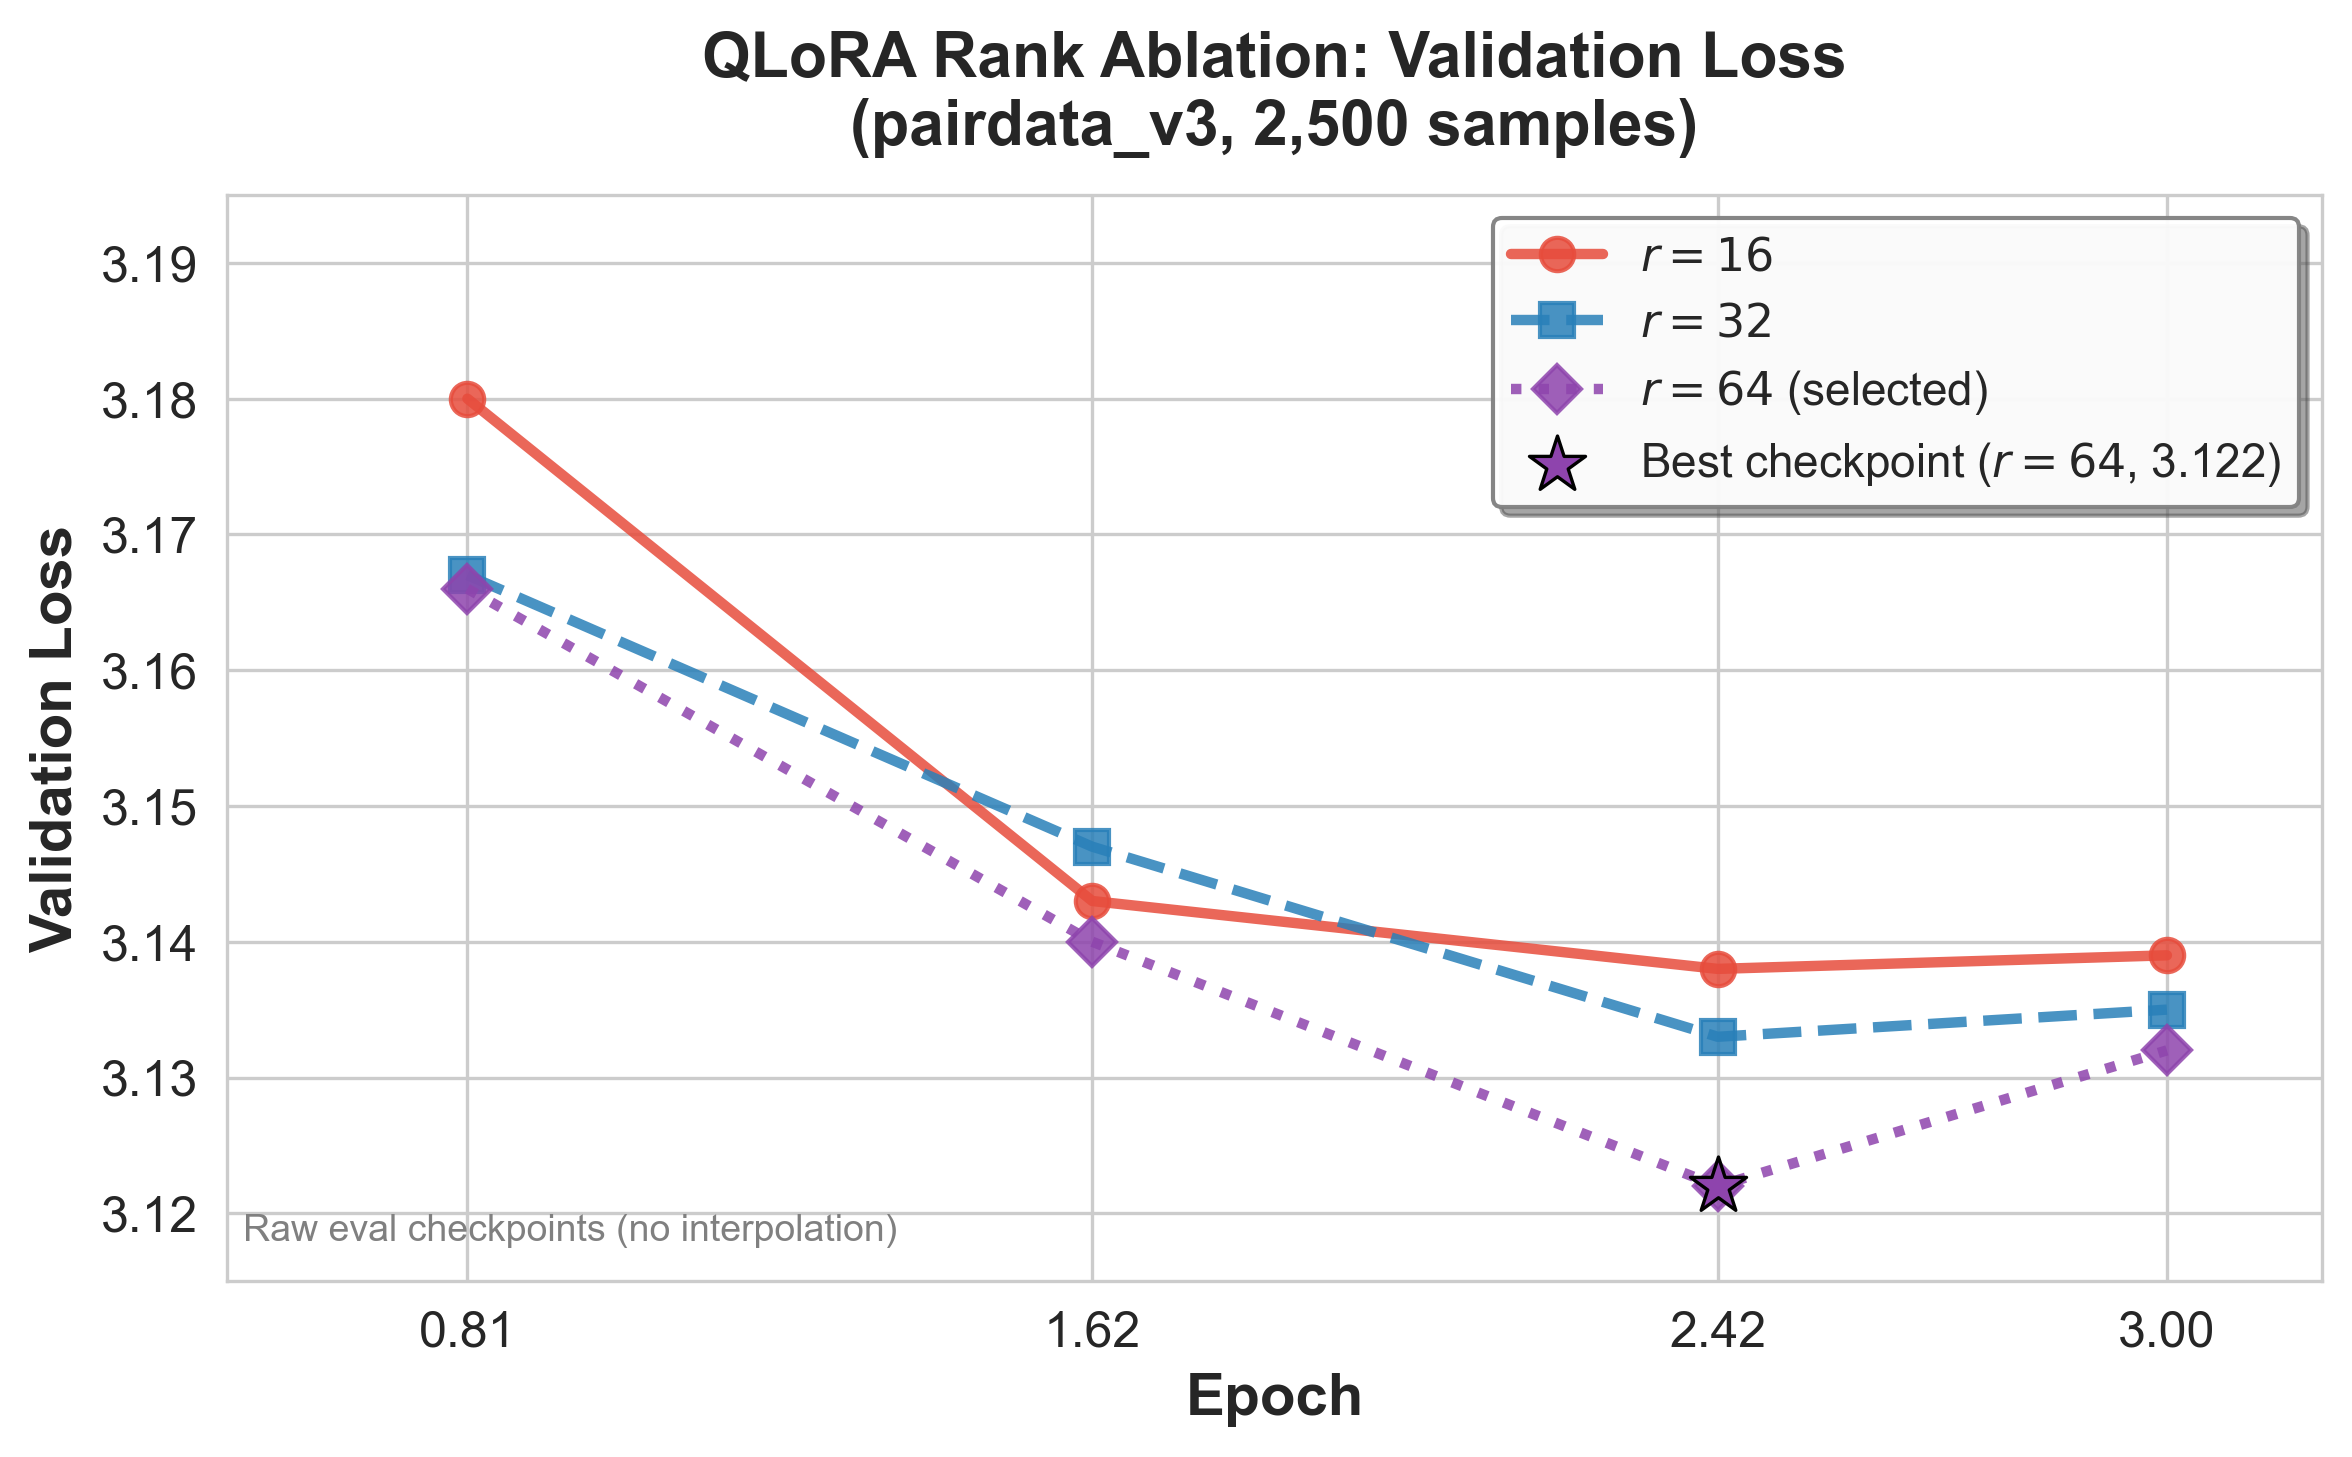
\includegraphics[width=0.55\columnwidth]{figures_vlm/21_u4_rank_ablation_pairdata_v3.png}
\caption{Validation loss trajectories for LoRA rank ablation on pairdata\_v3
(2\,500-sample scale, v0.8).
Points are plotted at raw evaluation checkpoints (no interpolation);
eval is performed after every 100 steps.
All three ranks reach their best checkpoint at epoch~2.421;
$r=64$ achieves the lowest validation loss of $3.122$, marked with a star~($\bigstar$).
The marginal uptick at epoch~3 for $r=64$ ($+0.010$ nats) suggests
the adapter is near its capacity limit at this scale,
underscoring the importance of best-checkpoint selection.}
\label{fig:u4_rank_ablation}
\end{figure}

\subsubsection*{Analysis: Optimal Rank Selection}

\paragraph{Monotonic improvement with rank.}
All three metrics---eval loss, token accuracy, and training loss---improve
monotonically as $r$ increases from 16 to 64:
\begin{itemize}
  \item \textbf{eval\_loss} (best ckpt): $3.138 \to 3.133 \to \mathbf{3.122}$
        ($\Delta = -0.016$ from r16 to r64, $-0.011$ from r32 to r64).
  \item \textbf{Token accuracy} (best ckpt): $98.73\,\% \to 98.83\,\% \to \mathbf{98.90\,\%}$.
  \item \textbf{Train loss} (final epoch): $3.567 \to 3.489 \to \mathbf{3.419}$,
        indicating that higher rank allows more expressive
        weight updates within the frozen-backbone regime.
\end{itemize}

\paragraph{Convergence profile.}
All three runs reach their best checkpoint at \textbf{epoch~2.421} (step~300
of 372), after which final-epoch values are marginally higher
(r16: $+0.001$; r32: $+0.002$; r64: $+0.010$).
This epoch-level pattern is visible in Figure~\ref{fig:u4_rank_ablation}:
all curves flatten after epoch~2.42 and the $r=64$ trajectory shows
the steepest final uptick, consistent with a near-capacity adapter.
The best-checkpoint selection strategy used by \texttt{SFTTrainer}
already captures the true minimum.

\paragraph{Computational cost.}
Despite quadrupling the trainable parameter count from r16
($42.3$\,M) to r64 ($168.8$\,M), the wall-clock time increases only from
3\,h\,24\,m to 3\,h\,27\,m on the RTX~4060~Ti~16\,GB.
The dominant cost is the frozen LLaVA-1.5-7B forward--backward pass, not
the adapter matrices; therefore r64 incurs virtually no extra VRAM or
latency overhead relative to r16.

\paragraph{Adapter capacity and domain specificity.}
The deeper convergence of $r=64$ at epoch~2.421 can be attributed to
\emph{sufficient parameter capacity for bridge-domain adaptation}.
With $168.8$\,M trainable parameters---$4.56$\,\% of the
7B frozen backbone---the LoRA adapter provides a wide enough
representation space to learn the fine-grained correspondence between
complex damage imagery and the structured recognition text that pairs
\emph{structural member type} (e.g., girder, slab, abutment) with
\emph{damage category} (e.g., cracking, rebar exposure, spalling).
By contrast, $r=16$ and $r=32$ constrain the adapter to only
$42.3$\,M and $84.7$\,M parameters respectively; these narrower
subspaces are insufficient to jointly represent the visual diversity
of bridge damage and the lexical structure of the target descriptions,
leaving a residual alignment gap that manifests as higher eval loss.
Put differently, bridge damage recognition requires the model to
simultaneously adapt its visual encoder--language decoder pathway
along multiple axes (member geometry, texture, crack pattern, color),
and a low-rank adapter with fewer degrees of freedom cannot span
all required directions in weight space.

\paragraph{Comparison with pairdata\_v2 baseline.}
The v0.8-r64 best eval loss (3.122) improves over the best pairdata\_v2
reference (3k, eval\_loss\,$=$\,3.135) by \textbf{$-0.013$}, and over the
2k reference (3.151) by \textbf{$-0.029$}, confirming that the pairdata\_v3
denoising pipeline and the 2{,}500-sample scale together yield a strictly
better training signal.

\paragraph{Conclusion: $r = 64$ selected as optimal.}
Based on this ablation, \textbf{$r = 64$} is selected as the LoRA rank for
all subsequent experiments:
\begin{enumerate}[label=(\roman*)]
  \item it achieves the lowest eval loss and highest token accuracy,
  \item it does not materially increase training time or VRAM usage, and
  \item it provides the strongest adapter for the DoRA comparison in
        Section~U.8, where the same rank is used to isolate the effect
        of magnitude--direction decomposition from rank capacity.
\end{enumerate}

\subsubsection*{Repro Commands}

\begin{verbatim}
# Activate training environment
.venv-train\Scripts\Activate.ps1

# LoRA rank ablation (r = 16, 32, 64) -- runs sequentially
python -u train_v08_qlora.py --lora-r 16 *> v08_r16_log.txt
python -u train_v08_qlora.py --lora-r 32 *> v08_r32_log.txt
python -u train_v08_qlora.py --lora-r 64 *> v08_r64_log.txt
\end{verbatim}

%%--------------------------------------------------------------------
\subsection*{U.5 Semantic Similarity Evaluation ($n=800$, Fixed Test Set)}
\label{sec:u5_similarity}
%%--------------------------------------------------------------------

\subsubsection*{Setup}

The fixed test set ($n=800$, \texttt{test\_set\_n800.csv}) used in all
prior evaluations is retained unchanged.
Ground-truth texts are replaced by pairdata\_v3 denoised versions---the
same Category~A/B/C pipeline applied to the test-set annotations.
The 2{,}048-dimensional composite evaluator
(\texttt{hotchpotch/static-embedding-japanese}~$\oplus$
\texttt{intfloat/multilingual-e5-large})
is used with unchanged tier thresholds:
Excellent~$\geq$\,0.85, Good~$\geq$\,0.70, Acceptable~$\geq$\,0.55,
Poor~$\geq$\,0.40, Very~Poor~$<$\,0.40.
Virtual environments: \texttt{.venv-pred} (inference),
\texttt{.venv-eval} (embedding evaluation).

\subsubsection*{Results}

\begin{table}[h]
\centering
\caption{Cosine similarity on pairdata\_v3 test set
         ($n=800$, 2{,}048-dim composite evaluator).
         LoRA rank ablation (v0.8) and DoRA (v0.9) results;
         pairdata-v2 reference from Supplementary~1.}
\label{tab:u5_similarity}
\setlength{\tabcolsep}{4pt}
\small
\begin{tabular}{lrrrrr}
\toprule
Model & $\bar{\rho}$ & $\sigma$ & Median & Good$+$ (\%) & V.\,Poor (\%) \\
\midrule
LoRA $r{=}16$ (v0.8) & 0.6464 & 0.0602 & 0.6480 & 18.9 & 0.0 \\
LoRA $r{=}32$ (v0.8) & 0.6700 & 0.0667 & 0.6689 & 32.9 & 0.0 \\
LoRA $r{=}64$ (v0.8) & 0.6571 & 0.0660 & 0.6606 & 28.4 & 0.0 \\
DoRA $r{=}64$ (v0.9) & \textbf{0.6846} & 0.0747 & \textbf{0.6835} & \textbf{41.0} & 0.0 \\
\midrule
\multicolumn{6}{l}{\textit{Reference: pairdata\_v2 results (Supplementary~1, Table~7)}} \\
2k (v0.7.5) & 0.6950 & 0.0824 & 0.7053 & 53.1 & 0.4 \\
3k (v0.7.3) & 0.6767 & 0.0751 & 0.6799 & 37.8 & 0.4 \\
\bottomrule
\end{tabular}
\end{table}

\subsubsection*{Repro Commands}

\begin{verbatim}
# Inference (n=800 test set, v0.8 model)
.venv-pred\Scripts\python.exe inference_v08_qlora.py \
    --test-csv data/v03_fine_tuning/test_set_n800.csv

# 2048-dim evaluation against pairdata_v3 GT
.venv-eval\Scripts\python.exe evaluate_2048dim_v08.py
\end{verbatim}

\begin{figure}[h]
  \centering
  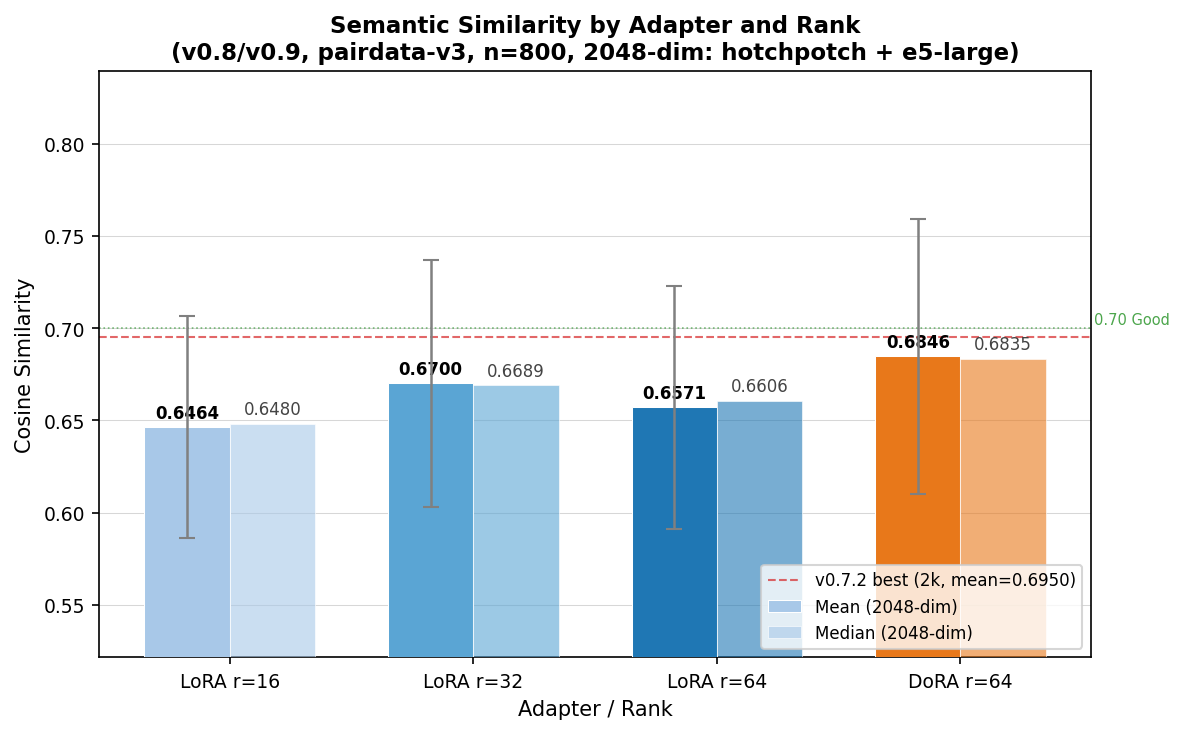
\includegraphics[width=0.85\linewidth]{figures_vlm/22_v08_similarity_by_adapter.png}
  \caption{Mean and median cosine similarity by adapter and rank
           (v0.8/v0.9, pairdata-v3, $n=800$, 2{,}048-dim composite evaluator).
           Error bars show $\pm1\sigma$. The dashed red line marks the best v0.7.2
           result (2k, mean\,=\,0.6950). DoRA $r{=}64$ achieves the highest mean
           (0.6846) among all tested adapters.}
  \label{fig:u5_similarity_by_adapter}
\end{figure}

\begin{figure}[h]
  \centering
  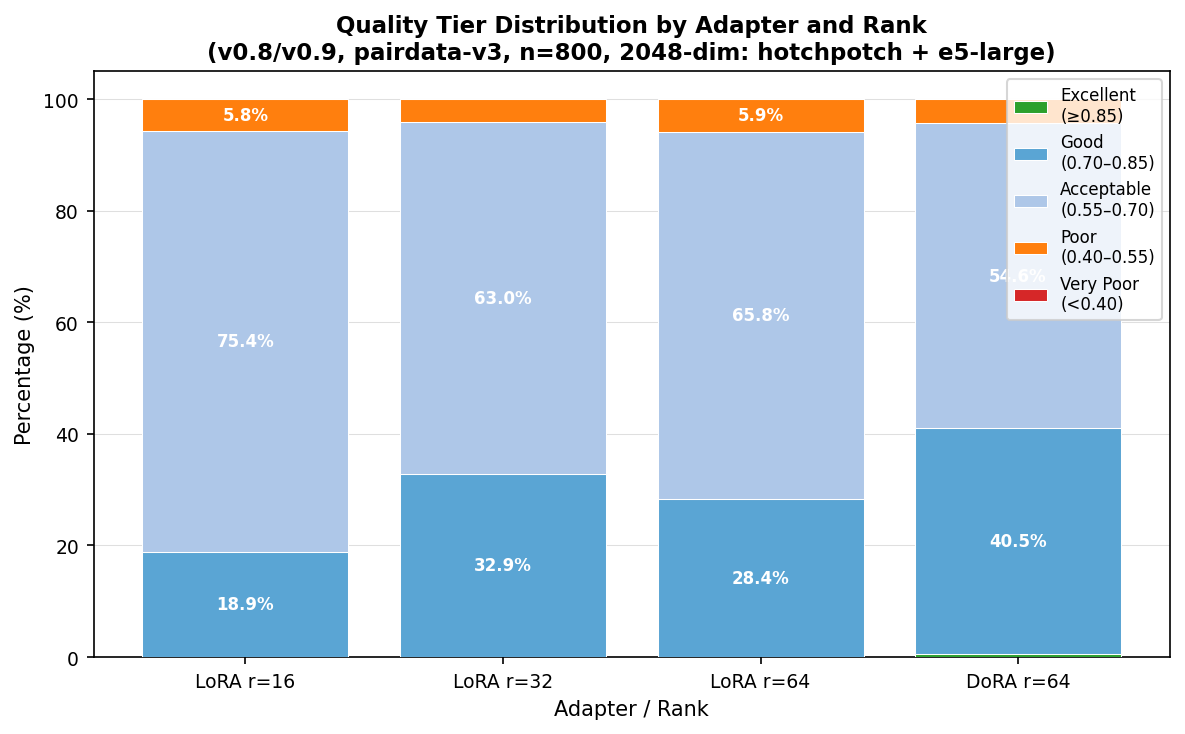
\includegraphics[width=0.85\linewidth]{figures_vlm/23_v08_tier_distribution.png}
  \caption{Quality tier distribution by adapter and rank.
           Good$+$ rate (Excellent $\cup$ Good $\cup$ Acceptable, $\geq$\,0.55)
           improves from 18.9\% (LoRA $r{=}16$) to 41.0\% (DoRA $r{=}64$).
           Very Poor samples ($<$\,0.40) are absent for all configurations.}
  \label{fig:u5_tier_distribution}
\end{figure}

\begin{figure}[h]
  \centering
  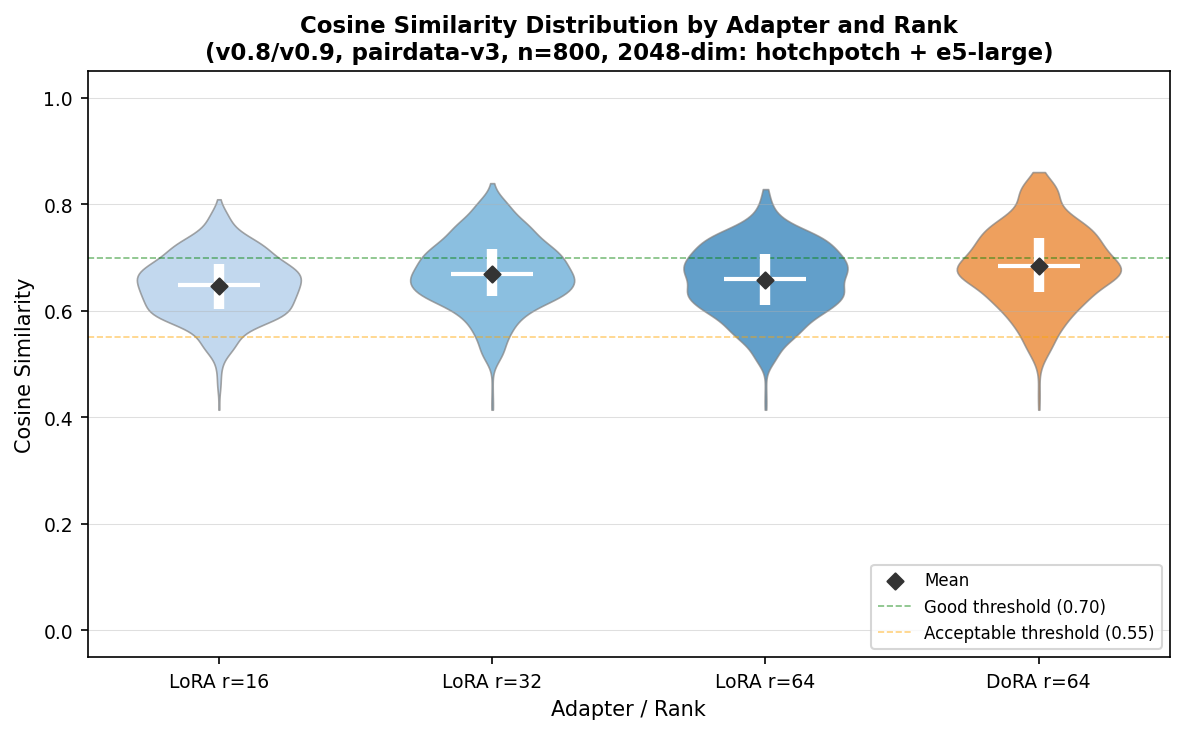
\includegraphics[width=0.85\linewidth]{figures_vlm/24_v08_cosine_violin.png}
  \caption{Distribution of cosine similarity scores across $n=800$ test samples.
           White box shows IQR; diamond marker shows the mean.
           Dashed lines indicate Good (0.70) and Acceptable (0.55) thresholds.
           DoRA $r{=}64$ shows a distribution shifted toward higher similarity
           compared with all LoRA rank variants.}
  \label{fig:u5_cosine_violin}
\end{figure}

\noindent\textbf{Analysis.}
Figure~\ref{fig:u5_similarity_by_adapter} shows that DoRA $r{=}64$ achieves
the highest mean cosine similarity (0.6846) among all tested adapters,
surpassing even the best LoRA variant ($r{=}32$, mean\,=\,0.6700).
This improvement is attributable to DoRA's weight decomposition into
magnitude and direction components, which enables finer-grained parameter
updates than standard LoRA.
Note that all v0.8/v0.9 results are evaluated on pairdata-v3 and are
therefore \emph{not directly comparable} to the v0.7.x reference values,
which were obtained on pairdata-v2.

Figure~\ref{fig:u5_tier_distribution} reveals a more pronounced difference
in the Good tier: DoRA $r{=}64$ achieves a Good$+$ rate of 41.0\%,
substantially higher than the best LoRA result of 32.9\% ($r{=}32$).
Based on embedding-similarity scores alone, DoRA $r{=}64$ achieves the
highest mean cosine similarity (0.6846) and Good$+$ rate (41.0\,\%).
The rank $r{=}64$ for DoRA was chosen to match the LoRA rank whose
validation loss guided the hyperparameter selection.
Among the LoRA variants, $r{=}32$ yields the best cosine similarity
(0.6700), ranking second overall.
Both LoRA $r{=}32$ and DoRA $r{=}64$ are forwarded to the Quality Guard
and Priority Scoring assessment in U.6 to determine whether the
embedding-level advantage of DoRA translates into a meaningful
downstream gain.

%%--------------------------------------------------------------------
\subsection*{U.6 Quality Guard Results (v0.8)}
\label{sec:u6_quality_guard}
%%--------------------------------------------------------------------

Quality Guard thresholds are retained from v0.7.3:
$\theta_{\mathrm{low}}=30$, $\theta_{\mathrm{high}}=200$.
Stage~2 (Swallow-8B SLM) is omitted; Stage~1 rule-based filter
alone was empirically sufficient (Supplementary~1, S.7).
The pipeline is applied to the two selected models:
\textbf{LoRA $r{=}32$ (v0.8)} and \textbf{DoRA $r{=}64$ (v0.9)}.
Virtual environment: \texttt{.venv-eval}.

\begin{table}[h]
\centering
\caption{Quality Guard results: LoRA $r{=}32$ (v0.8) and DoRA $r{=}64$ (v0.9)
         on pairdata-v3 test set ($n=800$, $\theta_{\mathrm{low}}=30$,
         $\theta_{\mathrm{high}}=200$).}
\label{tab:u6_qg_results}
\setlength{\tabcolsep}{4pt}
\small
\begin{tabular}{lrrrr}
\toprule
 & \multicolumn{2}{c}{LoRA $r{=}32$ (v0.8)} & \multicolumn{2}{c}{DoRA $r{=}64$ (v0.9)} \\
\cmidrule(lr){2-3}\cmidrule(lr){4-5}
\textbf{Verdict} & Count & Rate (\%) & Count & Rate (\%) \\
\midrule
PASS --- High Quality            & 798 & 99.8 & 798 & 99.8 \\
FAIL --- Too short / Error       &   2 &  0.2 &   2 &  0.2 \\
\midrule
\textbf{Total}                   & 800 & 100.0 & 800 & 100.0 \\
\midrule
\multicolumn{5}{l}{\textit{Reference (pairdata-v2)}} \\
v0.7.5 (2k) & \multicolumn{2}{r}{787\ (98.4\,\% PASS)} &
v0.7.3 (3k) & \multicolumn{1}{r}{787\ (98.4\,\%)} \\
\bottomrule
\end{tabular}
\end{table}

\begin{table}[h]
\centering
\caption{Priority level distribution for PASS predictions ($n=798$ each).
         Keyword-based structuring + priority scoring
         ($\theta_{\mathrm{low}}=30$, $\theta_{\mathrm{high}}=200$).}
\label{tab:u6_priority}
\setlength{\tabcolsep}{4pt}
\small
\begin{tabular}{lrrrr}
\toprule
 & \multicolumn{2}{c}{LoRA $r{=}32$ (v0.8)} & \multicolumn{2}{c}{DoRA $r{=}64$ (v0.9)} \\
\cmidrule(lr){2-3}\cmidrule(lr){4-5}
\textbf{Priority Level} & Count & (\%) & Count & (\%) \\
\midrule
Level~3 (Planned maintenance) &  64 &  8.0 &   0 &  0.0 \\
Level~4 (Priority repair)     & 632 & 79.2 & 798 & 100.0 \\
Level~5 (Immediate repair)    & 102 & 12.8 &   0 &  0.0 \\
\midrule
\textbf{Total PASS}           & 798 & 100.0 & 798 & 100.0 \\
\bottomrule
\end{tabular}
\end{table}

\noindent\textbf{Analysis.}
Both models achieve a PASS rate of 99.8\,\%, surpassing the pairdata-v2
reference (98.4\,\%).  The two FAIL cases per model are file-not-found
error strings and do not reflect model-quality failures.

\paragraph{Token count distribution (Figure~\ref{fig:u6_token}).}
LoRA $r{=}32$ produces a broad token-count distribution
(mean\,=\,90, $\sigma$\,=\,19, max\,=\,182), indicating diverse
output lengths adapted to image content.
DoRA $r{=}64$, by contrast, exhibits extreme concentration
(mean\,=\,84, $\sigma$\,=\,4.5, $p_5=p_{95}=84$): virtually every
prediction is 84 tokens, a near-degenerate distribution consistent
with output-level mode collapse.

\paragraph{Priority level distribution (Figure~\ref{fig:u6_priority}).}
LoRA $r{=}32$ distributes across Level~3 (8.0\,\%), Level~4 (79.2\,\%),
and Level~5 (12.8\,\%).  Compared with the pairdata-v2 reference
(v0.7.3 3k: Level~3 2.7\,\%, Level~4 82.7\,\%, Level~5 14.6\,\%),
LoRA $r{=}32$ shows an increased Level~3 share---suggesting
that pairdata-v3 training yields more balanced severity assignment
rather than a bias toward high-urgency predictions.
DoRA $r{=}64$ assigns \emph{all} 798 PASS predictions to Level~4
(100.0\,\%), with Level~3 and Level~5 both absent.
This complete absence of severity variation is a further indicator of
output-level mode collapse: the model produces a single stereotyped
template regardless of image content.

\paragraph{Conclusion: DoRA $r{=}64$ fine-tuning failure.}
The combination of extreme token uniformity ($\sigma=4.5$), total
priority-level collapse (Level~4 100\,\%), and complete absence of
semantic diversity (see U.6.1) indicates that the DoRA $r{=}64$
fine-tuning was unsuccessful as a practical damage-assessment model.
A likely cause is that the rank $r{=}64$ setting---chosen to match
the LoRA ablation condition guided by validation loss---was
excessive for DoRA, whose weight-decomposition mechanism may require
smaller rank values to converge to a diverse output distribution.
Establishing a reliable DoRA fine-tuning protocol, including
hyperparameter search over rank, learning rate, and adapter scale,
is left as future work.
\textbf{LoRA $r{=}32$ (v0.8) is therefore adopted as the final
downstream pipeline model.}

Figure~\ref{fig:u6_token} shows the token-count histograms.
Figure~\ref{fig:u6_guard} compares the PASS/FAIL verdicts and reason codes.
Figure~\ref{fig:u6_priority} illustrates the priority composition difference.

\begin{figure}[h]
  \centering
  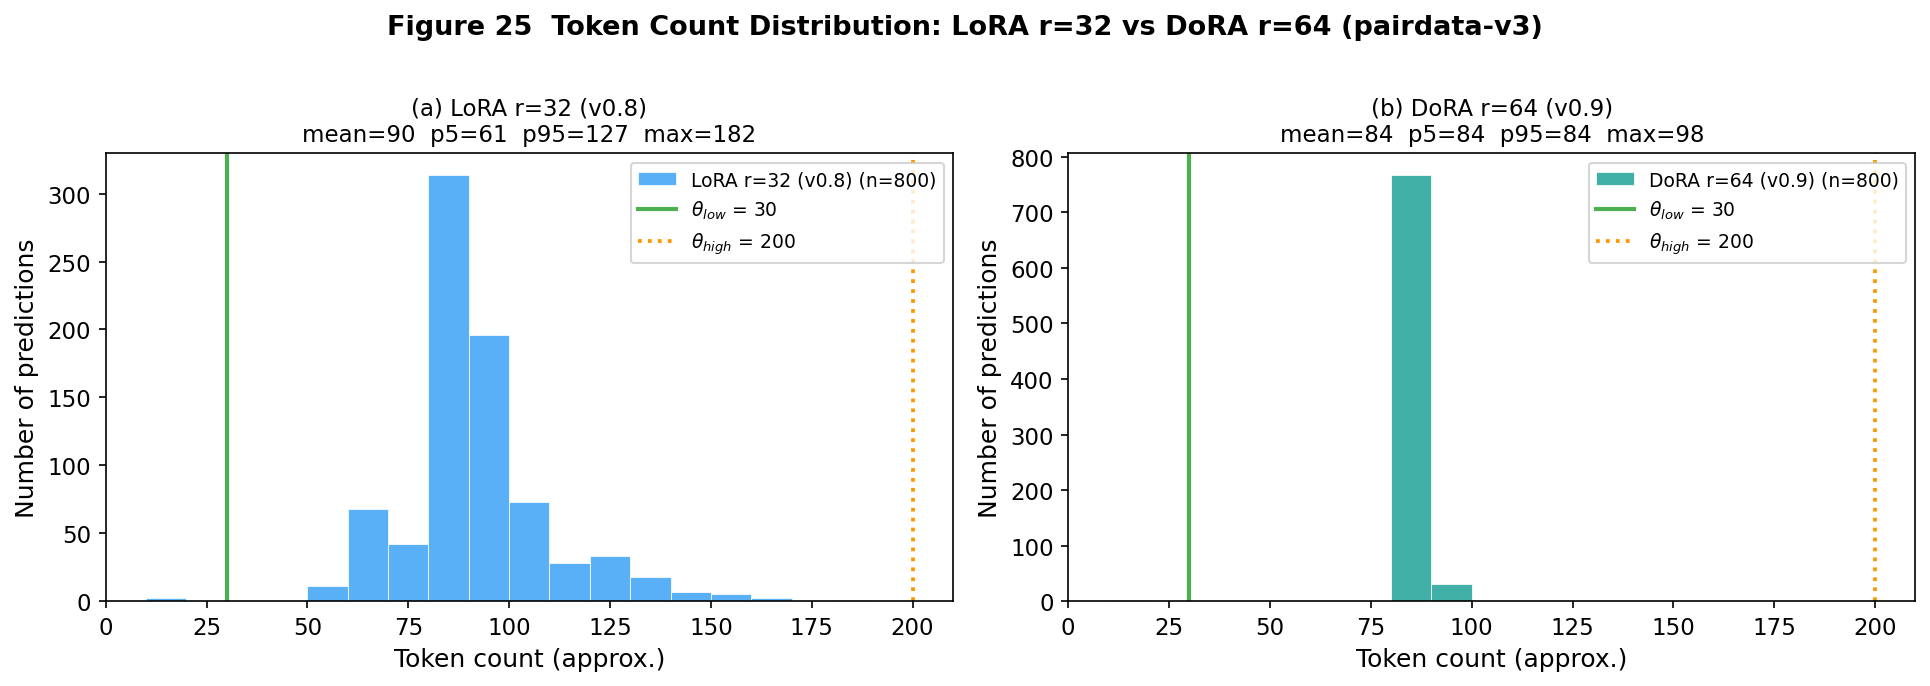
\includegraphics[width=0.92\linewidth]{figures_vlm/25_v08_token_distribution.png}
  \caption{Token count distributions: LoRA $r{=}32$ (left) and DoRA $r{=}64$ (right).
           Solid green: $\theta_{\mathrm{low}}=30$; dotted orange: $\theta_{\mathrm{high}}=200$.
           LoRA $r{=}32$ shows a broad distribution (mean\,=\,90, $\sigma$\,=\,19, max\,=\,182);
           DoRA $r{=}64$ exhibits extreme concentration (mean\,=\,84, $\sigma$\,=\,4.5,
           $p_5=p_{95}=84$), indicating near-uniform output length.}
  \label{fig:u6_token}
\end{figure}

\begin{figure}[h]
  \centering
  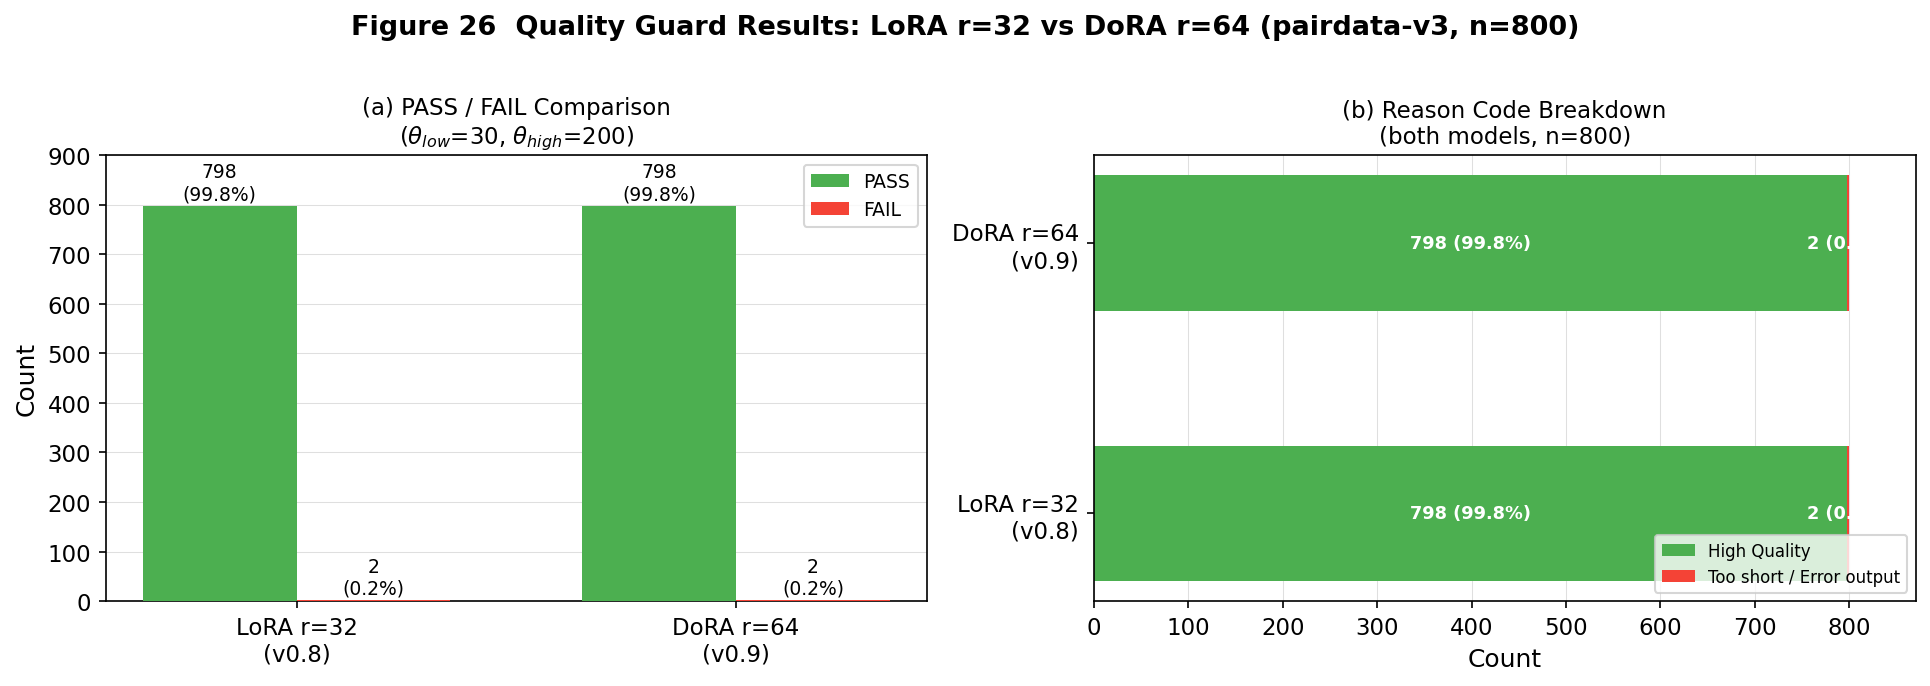
\includegraphics[width=0.92\linewidth]{figures_vlm/26_v08_guard_breakdown.png}
  \caption{Quality Guard results (pairdata-v3, $n=800$).
           \textit{(a)} PASS/FAIL comparison: both models achieve 99.8\,\% PASS,
           exceeding the pairdata-v2 reference (98.4\,\%).
           \textit{(b)} Reason code breakdown: both models produce only
           ``High Quality'' and ``Too short / Error output'' codes (2 each).}
  \label{fig:u6_guard}
\end{figure}

\begin{figure}[h]
  \centering
  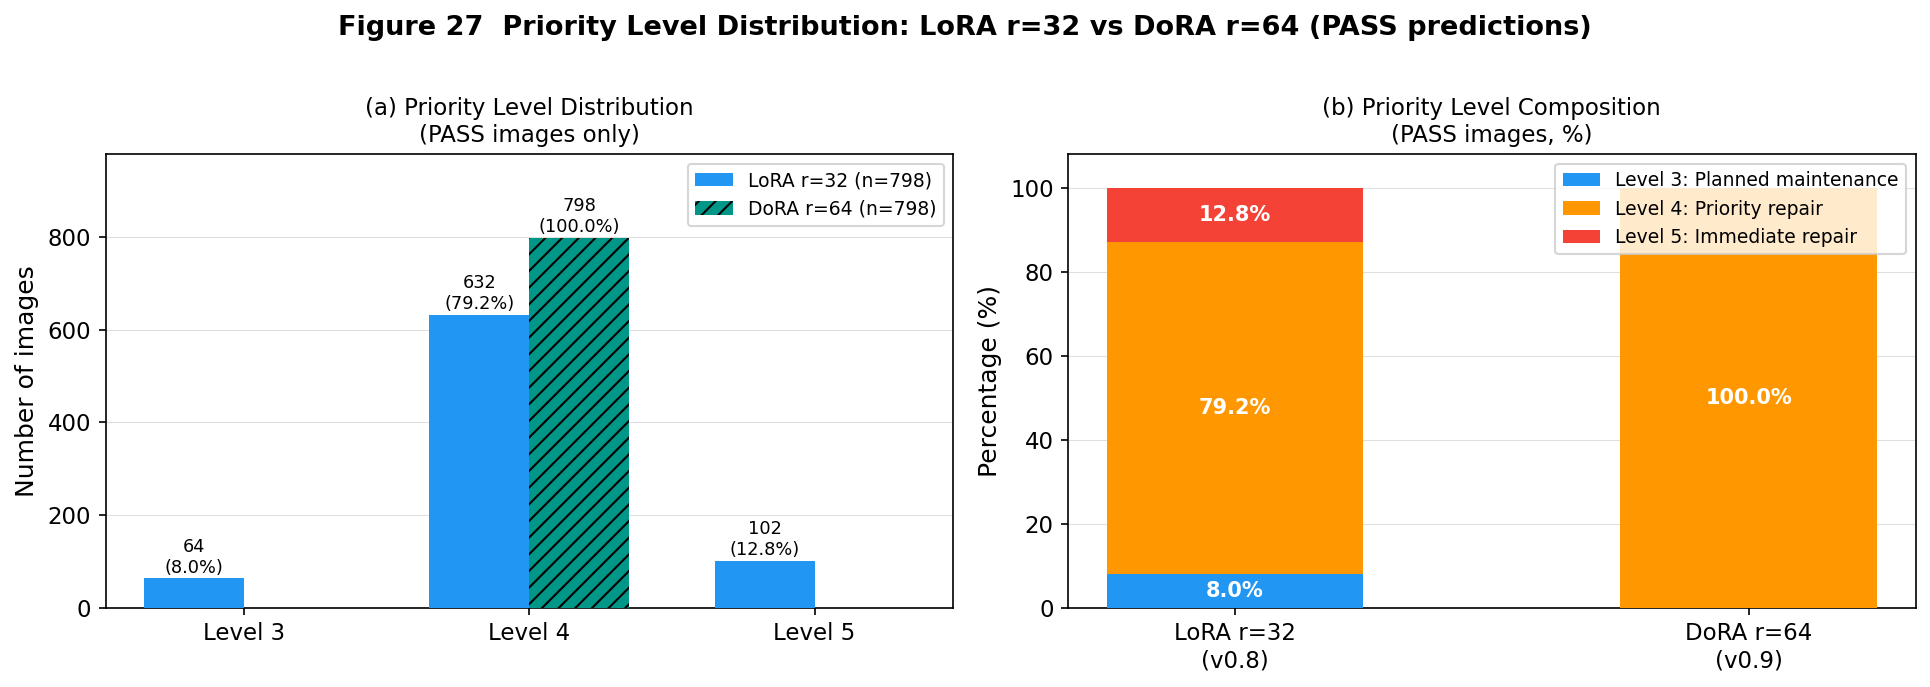
\includegraphics[width=0.92\linewidth]{figures_vlm/27_v08_priority_distribution.png}
  \caption{Priority level distribution for PASS predictions ($n=798$).
           \textit{(a)} Grouped bar chart; \textit{(b)} stacked percentage view.
           LoRA $r{=}32$ distributes across Level~3--5; DoRA $r{=}64$ concentrates
           entirely at Level~4 (100.0\,\%), reflecting output-level uniformity.}
  \label{fig:u6_priority}
\end{figure}

%%--------------------------------------------------------------------
\subsection*{U.6.1\quad Structural Member and Damage Type: pairdata v3,
             LoRA $r{=}32$ vs.\ DoRA $r{=}64$}
\label{sec:u61_member_damage}
%%--------------------------------------------------------------------

Following the same methodology as S.7.1 (Supplementary~1), we apply
keyword-based structural member and damage-type extraction to the
PASS predictions of both models on pairdata-v3
(Figure~\ref{fig:u61_member_damage}).

\begin{figure}[H]
\centering
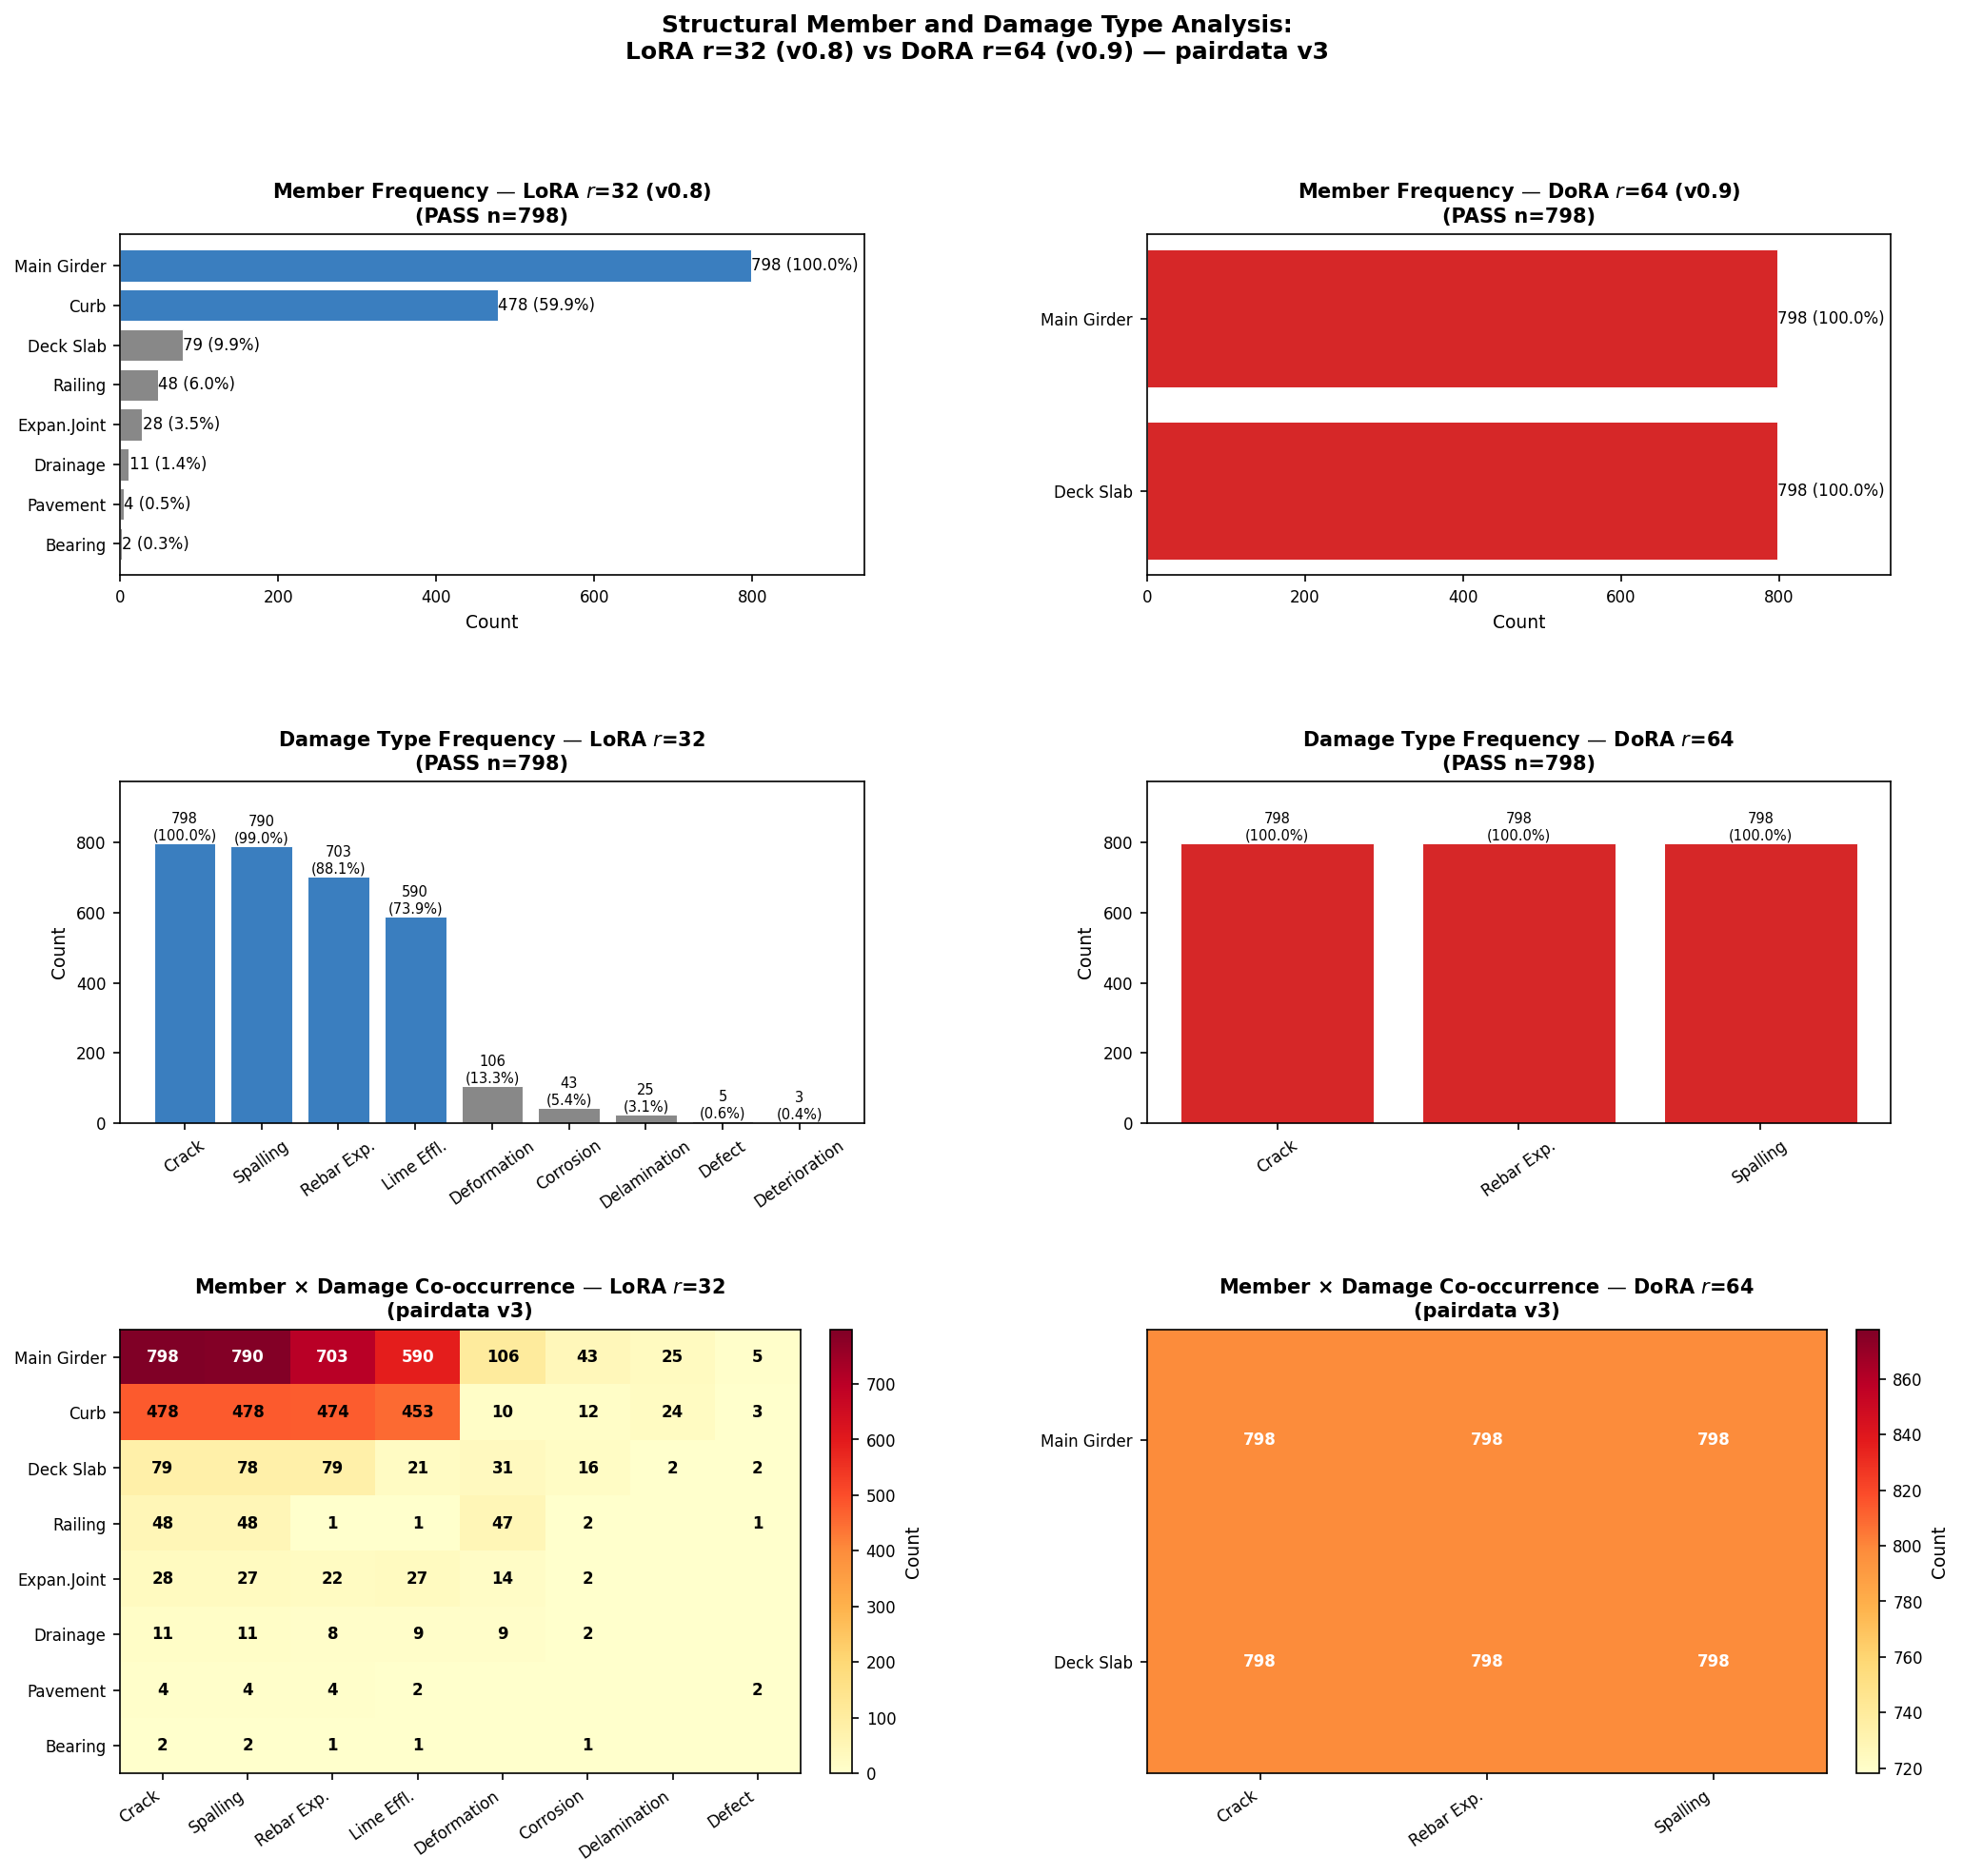
\includegraphics[width=0.9\textwidth]{figures_vlm/28_v08_member_damage_r32_dora.png}
\caption{Structural member and damage type analysis for PASS predictions
         on pairdata-v3 ($n=798$ each):
         \textit{left column} LoRA $r{=}32$ (v0.8, blue),
         \textit{right column} DoRA $r{=}64$ (v0.9, red).
         \textit{Top}: structural member mention frequency;
         \textit{Middle}: damage type frequency;
         \textit{Bottom}: member $\times$ damage co-occurrence heatmap.}
\label{fig:u61_member_damage}
\end{figure}

\paragraph{Member distribution.}
LoRA $r{=}32$ reproduces the pairdata-v2 pattern: Main Girder dominates
(100\,\%) with Curb as secondary (60.0\,\%), reflecting the
image-specific localization introduced by pairdata-v3.
DoRA $r{=}64$ produces a degenerate member distribution: Main Girder
and Deck Slab both appear at 100.0\,\%, with no other member ever
mentioned.  This rigid two-member template is independent of image
content and confirms stereotyped generation.

\paragraph{Damage type distribution.}
LoRA $r{=}32$ captures vocabulary diversity---Crack (100\,\%),
Spalling (99.0\,\%), Rebar Exposure (88.1\,\%), Lime Efflorescence
(73.9\,\%), with secondary types (Deformation 13.3\,\%, Corrosion
5.4\,\%) reflecting image-dependent variation.
DoRA $r{=}64$ assigns Crack, Rebar Exposure, and Spalling each
at 100.0\,\%, with no other damage type present.
The complete co-occurrence collapse---every prediction contains
identical member and damage keywords---is the structural manifestation
of the token and priority uniformity observed in U.6 and constitutes
clear evidence of fine-tuning failure for DoRA $r{=}64$.

%%--------------------------------------------------------------------
\clearpage
\section*{U.7\quad Qualitative Analysis: Representative PASS Predictions}
\label{sec:u7}
%%--------------------------------------------------------------------

Figures~\ref{fig:u7_pass_1}--\ref{fig:u7_pass_3} present twelve representative
PASS predictions produced by the v0.8 LoRA~$r{=}32$ pipeline on pairdata~v3.
Images are selected to cover a range of structural members and damage types.
Each sub-caption shows the pairdata~v3 ground truth (\textbf{GT}),
the pipeline output (\textbf{Pred}),
and three quality indicators:
\textit{Sim(emb)} (2048-dim composite embedding cosine similarity),
\textit{Priority Score} (continuous scorer output, 0--1 scale), and
\textit{Level} (priority tier: 3~=~Planned, 4~=~Priority, 5~=~Immediate).

\begin{figure}[H]
  \centering
  \begin{minipage}[t]{0.46\textwidth}
    {\centering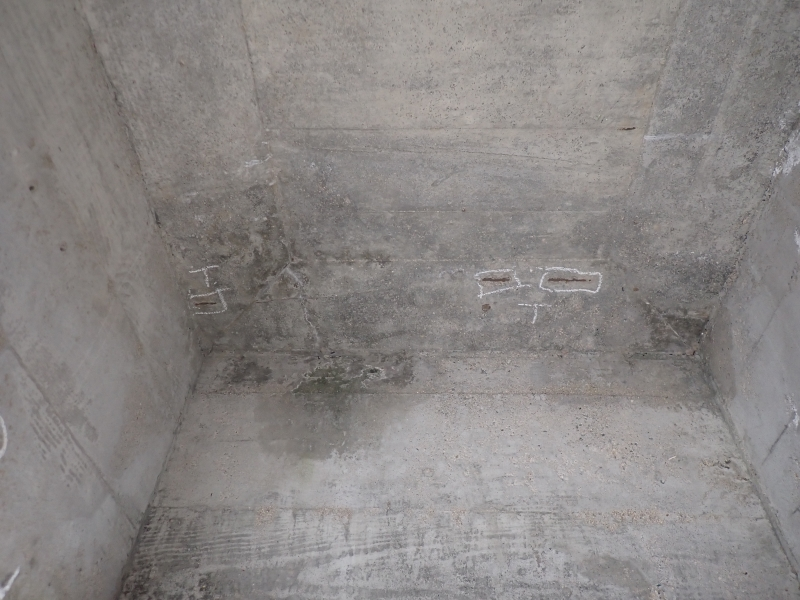
\includegraphics[width=0.675\linewidth]{figures_vlm/s8/s8_01_girder_cracking.jpg}\par}
    \vspace{2pt}
    {\scriptsize\raggedright
    \textbf{Quality Metrics:}~\textit{Sim(emb):~0.840;\enspace Priority:~1.00;\enspace Level:~5}\\[1pt]
    \textbf{GT:} \begin{CJK}{UTF8}{ipxm}{\CJKfamily{ipxg}主桁}に{\CJKfamily{ipxg}ひびわれ}（最大W=0.3mm)・{\CJKfamily{ipxg}鉄筋露出}・{\CJKfamily{ipxg}うき}・{\CJKfamily{ipxg}遊離石灰}・漏水跡、{\CJKfamily{ipxg}床版}に{\CJKfamily{ipxg}鉄筋露出}・破損・剥離・{\CJKfamily{ipxg}遊離石灰}が見られる。{\CJKfamily{ipxg}主桁}の損傷は、鉄筋の被り不足及び中性化・コンクリートの低品質、{\CJKfamily{ipxg}床版}の損傷は、鉄筋の被り不足・防護柵の施工が原因と考えられる。前回点検から{\CJKfamily{ipxg}鉄筋露出}に進展が見られるため、経過観察を行い、状況により補修を行う。\end{CJK}\\[1pt]
    \textbf{Pred:} \begin{CJK}{UTF8}{ipxm}{\CJKfamily{ipxg}主桁}に{\CJKfamily{ipxg}ひびわれ}、{\CJKfamily{ipxg}うき}が見られる。また、{\CJKfamily{ipxg}鉄筋露出}もみられる。{\CJKfamily{ipxg}床版}はかぶり不足が原因と思われる{\CJKfamily{ipxg}鉄筋露出}が多数みられる。間詰め部分から錆汁を伴う{\CJKfamily{ipxg}遊離石灰}が見られる。車両通行時には危険性があるため早期措置が望ましい。\end{CJK}
    \par}
  \end{minipage}
  \hfill
  \begin{minipage}[t]{0.46\textwidth}
    {\centering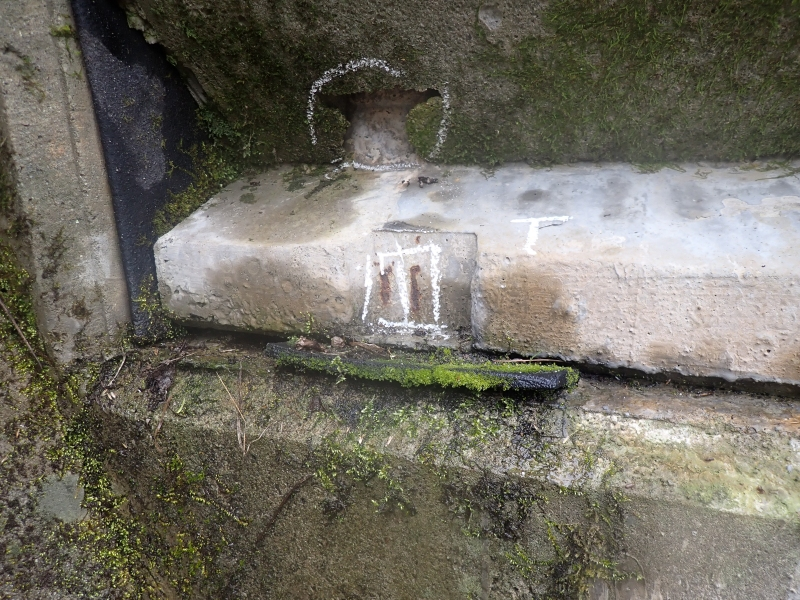
\includegraphics[width=0.675\linewidth]{figures_vlm/s8/s8_02_girder_rebar_exposure.jpg}\par}
    \vspace{2pt}
    {\scriptsize\raggedright
    \textbf{Quality Metrics:}~\textit{Sim(emb):~0.808;\enspace Priority:~0.81;\enspace Level:~4}\\[1pt]
    \textbf{GT:} \begin{CJK}{UTF8}{ipxm}{\CJKfamily{ipxg}主桁}に{\CJKfamily{ipxg}鉄筋露出}、間詰めに漏水・{\CJKfamily{ipxg}遊離石灰}が見られる。{\CJKfamily{ipxg}主桁}の{\CJKfamily{ipxg}鉄筋露出}は被り不足、間詰めの損傷は、橋面からの漏水が原因と考えられる。{\CJKfamily{ipxg}主桁}の損傷は前回確認されていないが局所的である。道路橋の機能に支障は生じていないため、次回点検時に状況の確認を行う。\end{CJK}\\[1pt]
    \textbf{Pred:} \begin{CJK}{UTF8}{ipxm}{\CJKfamily{ipxg}主桁}にひびわれ、うきが見られる。また、{\CJKfamily{ipxg}鉄筋露出}もみられる。間詰め部から{\CJKfamily{ipxg}遊離石灰}（錆汁）が析出している。橋面からの水分の侵入や地覆からの伝い水等が原因と思われる。局所的である為，経過観察とする。\end{CJK}
    \par}
  \end{minipage}
  \\[4pt]
  \begin{minipage}[t]{0.46\textwidth}
    {\centering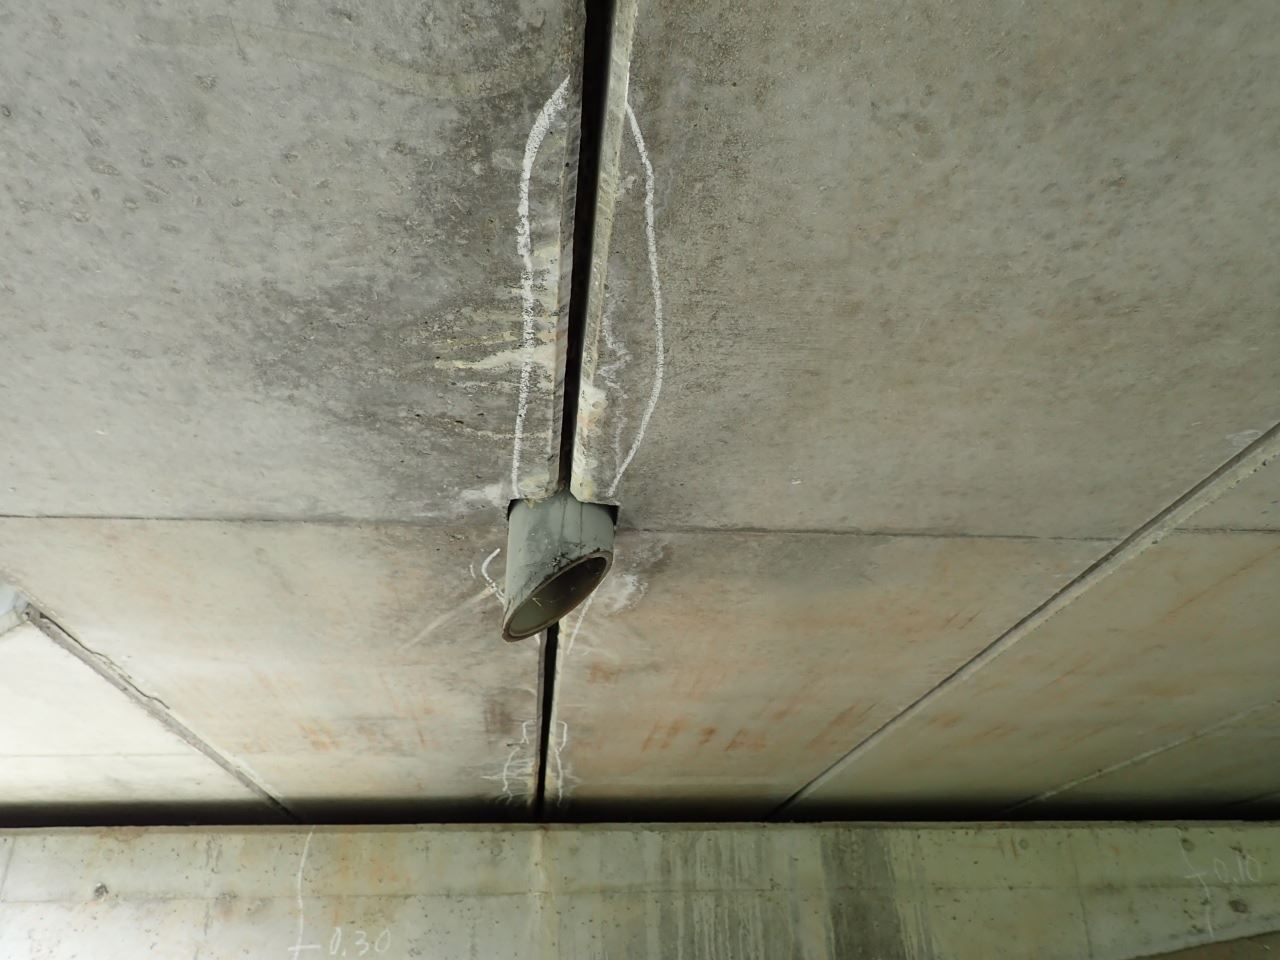
\includegraphics[width=0.675\linewidth]{figures_vlm/s8/s8_03_girder_spalling.jpg}\par}
    \vspace{2pt}
    {\scriptsize\raggedright
    \textbf{Quality Metrics:}~\textit{Sim(emb):~0.774;\enspace Priority:~0.81;\enspace Level:~4}\\[1pt]
    \textbf{GT:} \begin{CJK}{UTF8}{ipxm}{\CJKfamily{ipxg}主桁}に後埋めモルタルの剥離・鋼材露出、間詰めに一部{\CJKfamily{ipxg}錆}汁を伴う{\CJKfamily{ipxg}遊離石灰}が見られる。経過観察を行い、状況により補修を行う。\end{CJK}\\[1pt]
    \textbf{Pred:} \begin{CJK}{UTF8}{ipxm}{\CJKfamily{ipxg}主桁}にひびわれ、うきが見られる。また、鉄筋露出もみられる。間詰め部から{\CJKfamily{ipxg}遊離石灰}（{\CJKfamily{ipxg}錆}汁）が析出している。添加物の目地板に表面的な腐食が見られる。\end{CJK}
    \par}
  \end{minipage}
  \hfill
  \begin{minipage}[t]{0.46\textwidth}
    {\centering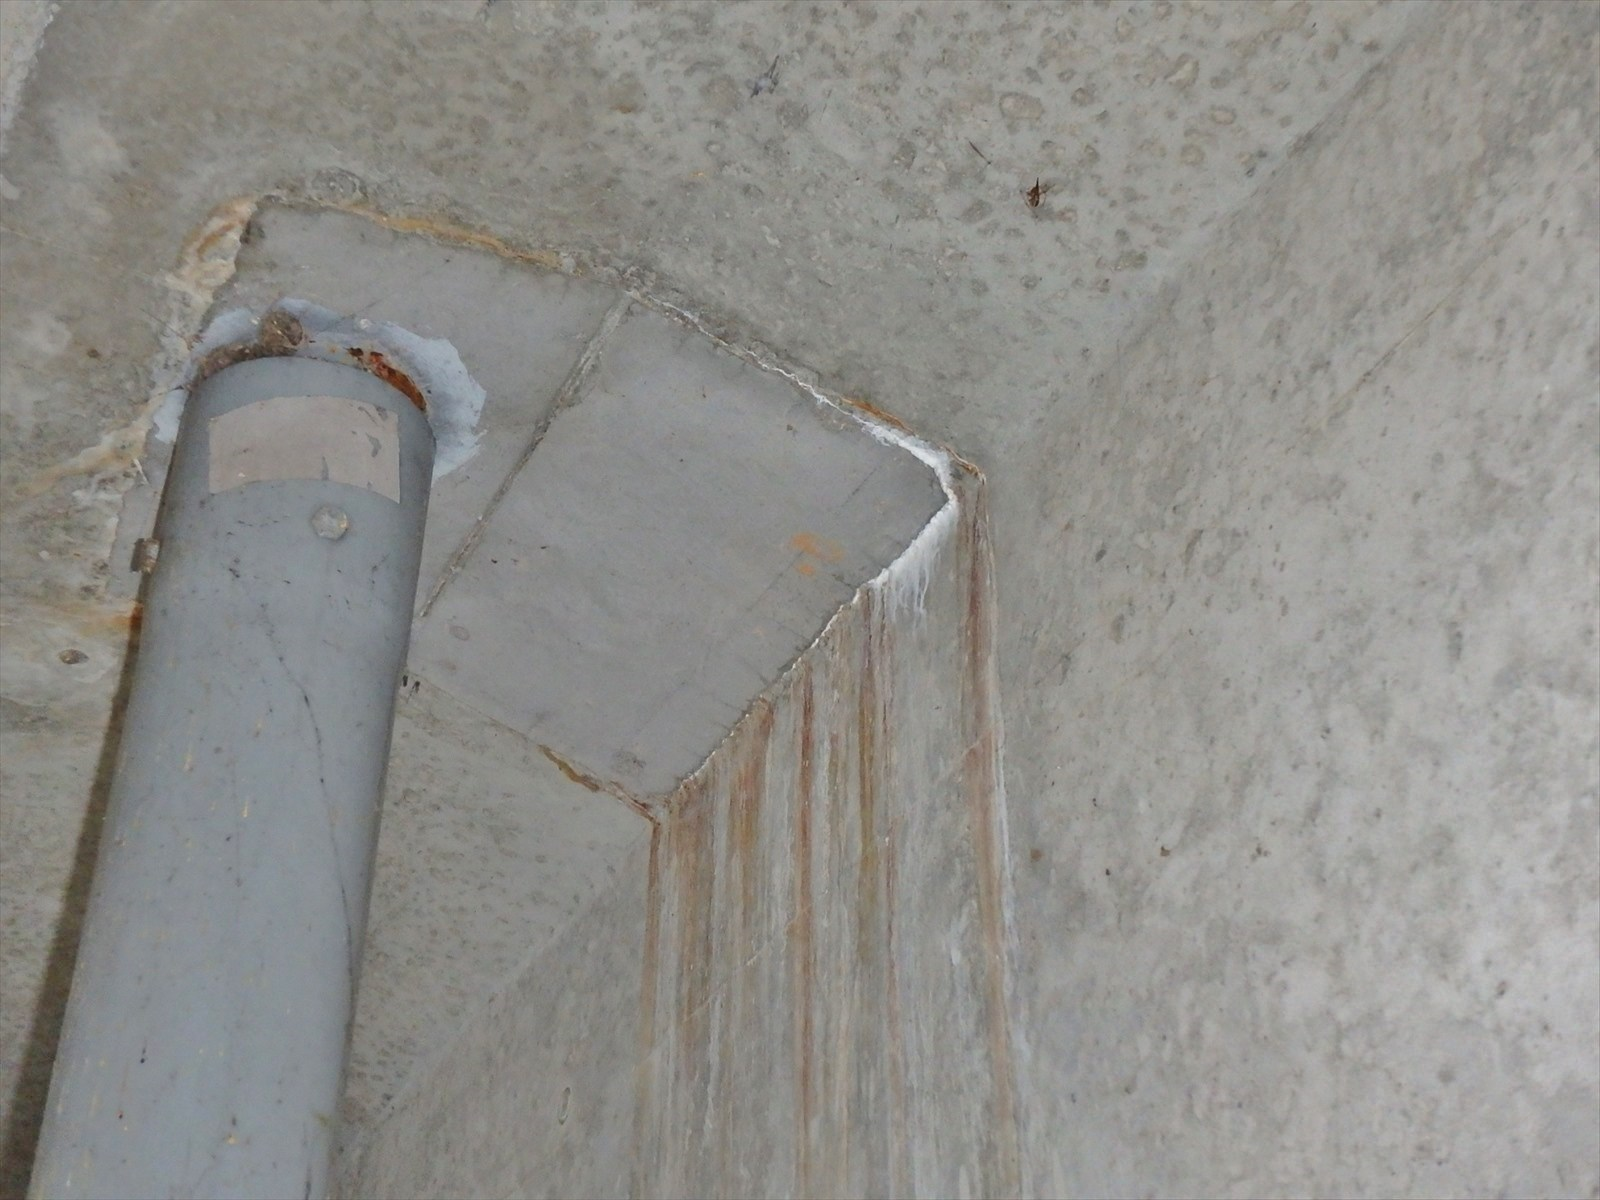
\includegraphics[width=0.675\linewidth]{figures_vlm/s8/s8_04_girder_corrosion.jpg}\par}
    \vspace{2pt}
    {\scriptsize\raggedright
    \textbf{Quality Metrics:}~\textit{Sim(emb):~0.713;\enspace Priority:~0.81;\enspace Level:~4}\\[1pt]
    \textbf{GT:} \begin{CJK}{UTF8}{ipxm}{\CJKfamily{ipxg}主桁}に漏水跡（{\CJKfamily{ipxg}錆}汁）が見られる。損傷は状況に応じて補修を行う事が望ましい。\end{CJK}\\[1pt]
    \textbf{Pred:} \begin{CJK}{UTF8}{ipxm}{\CJKfamily{ipxg}主桁}にひびわれ、うきが見られる。また、鉄筋露出もみられる。間詰め部から遊離石灰（{\CJKfamily{ipxg}錆}汁）が析出している。橋面からの水分の侵入や地覆からの伝い水等が原因と思われる。\end{CJK}
    \par}
  \end{minipage}
  \caption{Representative PASS predictions (1/3). \textbf{GT}: pairdata~v3 ground truth (Japanese); \textbf{Pred}: v0.8 LoRA~$r{=}32$ output; \textit{Sim(emb)}: 2048-dim composite cosine similarity; \textit{Priority}: scorer output; \textit{Level}: priority tier.}
  \label{fig:u7_pass_1}
\end{figure}
\clearpage
\begin{figure}[H]
  \centering
  \begin{minipage}[t]{0.46\textwidth}
    {\centering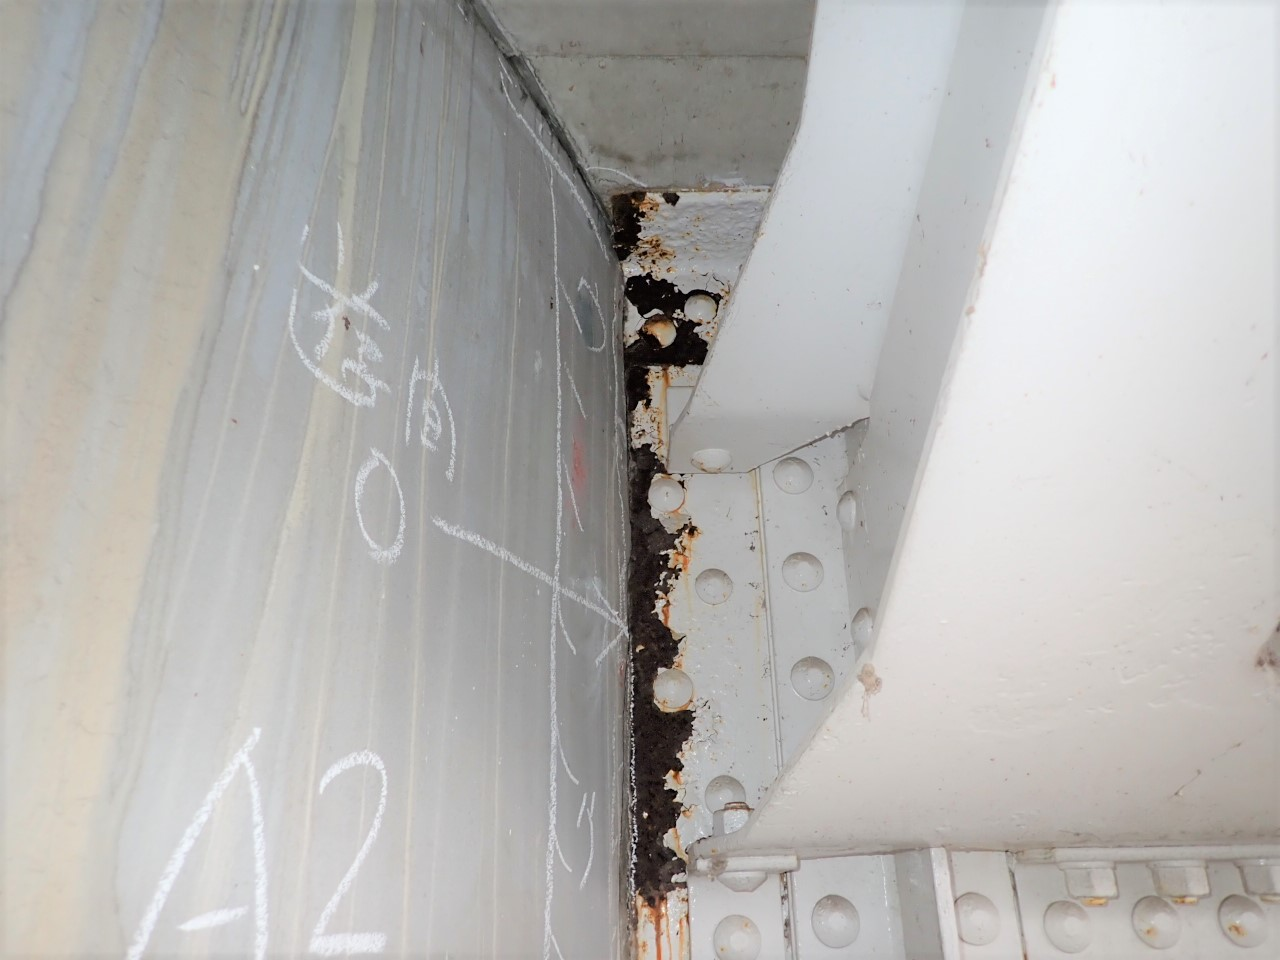
\includegraphics[width=0.675\linewidth]{figures_vlm/s8/s8_05_girder_settlement.jpg}\par}
    \vspace{2pt}
    {\scriptsize\raggedright
    \textbf{Quality Metrics:}~\textit{Sim(emb):~0.572;\enspace Priority:~0.81;\enspace Level:~4}\\[1pt]
    \textbf{GT:} \begin{CJK}{UTF8}{ipxm}伸縮装置にゴムの変形、A2橋台パラペットと{\CJKfamily{ipxg}主桁}の接触が見られる。経過観察を行い、状況により補修を行う。\end{CJK}\\[1pt]
    \textbf{Pred:} \begin{CJK}{UTF8}{ipxm}{\CJKfamily{ipxg}主桁}にひびわれ、うきが見られる。また、鉄筋露出もみられる。間詰め部から遊離石灰（錆汁）が析出している。橋面からの水分の侵入や地覆からの伝い水等が原因と思われる。\end{CJK}
    \par}
  \end{minipage}
  \hfill
  \begin{minipage}[t]{0.46\textwidth}
    {\centering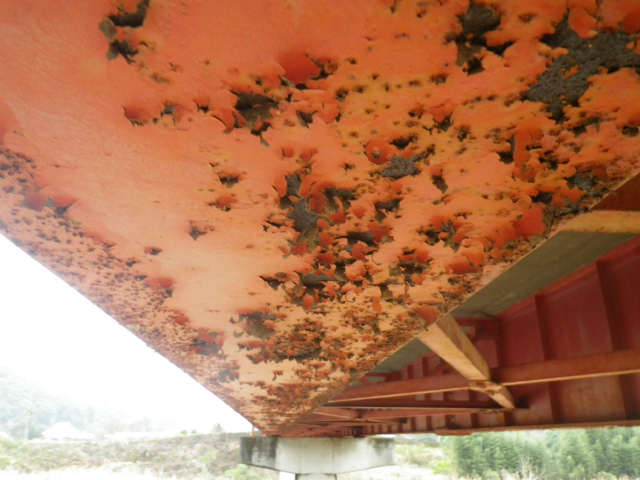
\includegraphics[width=0.675\linewidth]{figures_vlm/s8/s8_06_girder_other.jpg}\par}
    \vspace{2pt}
    {\scriptsize\raggedright
    \textbf{Quality Metrics:}~\textit{Sim(emb):~0.585;\enspace Priority:~0.81;\enspace Level:~4}\\[1pt]
    \textbf{GT:} \begin{CJK}{UTF8}{ipxm}{\CJKfamily{ipxg}主桁}・横桁に塗装剥がれや防食機能の劣化が認められる\end{CJK}\\[1pt]
    \textbf{Pred:} \begin{CJK}{UTF8}{ipxm}{\CJKfamily{ipxg}主桁}にひびわれ、うきが見られる。また、鉄筋露出もみられる。間詰め部から遊離石灰（錆汁）が析出している。橋面からの水分の侵入や地覆からの伝い水等が原因と思われる。高力ボルト・ナットは使用中であり、今後継目材の変更等によって止水機能の向上を行う必要がある。\end{CJK}
    \par}
  \end{minipage}
  \\[4pt]
  \begin{minipage}[t]{0.46\textwidth}
    {\centering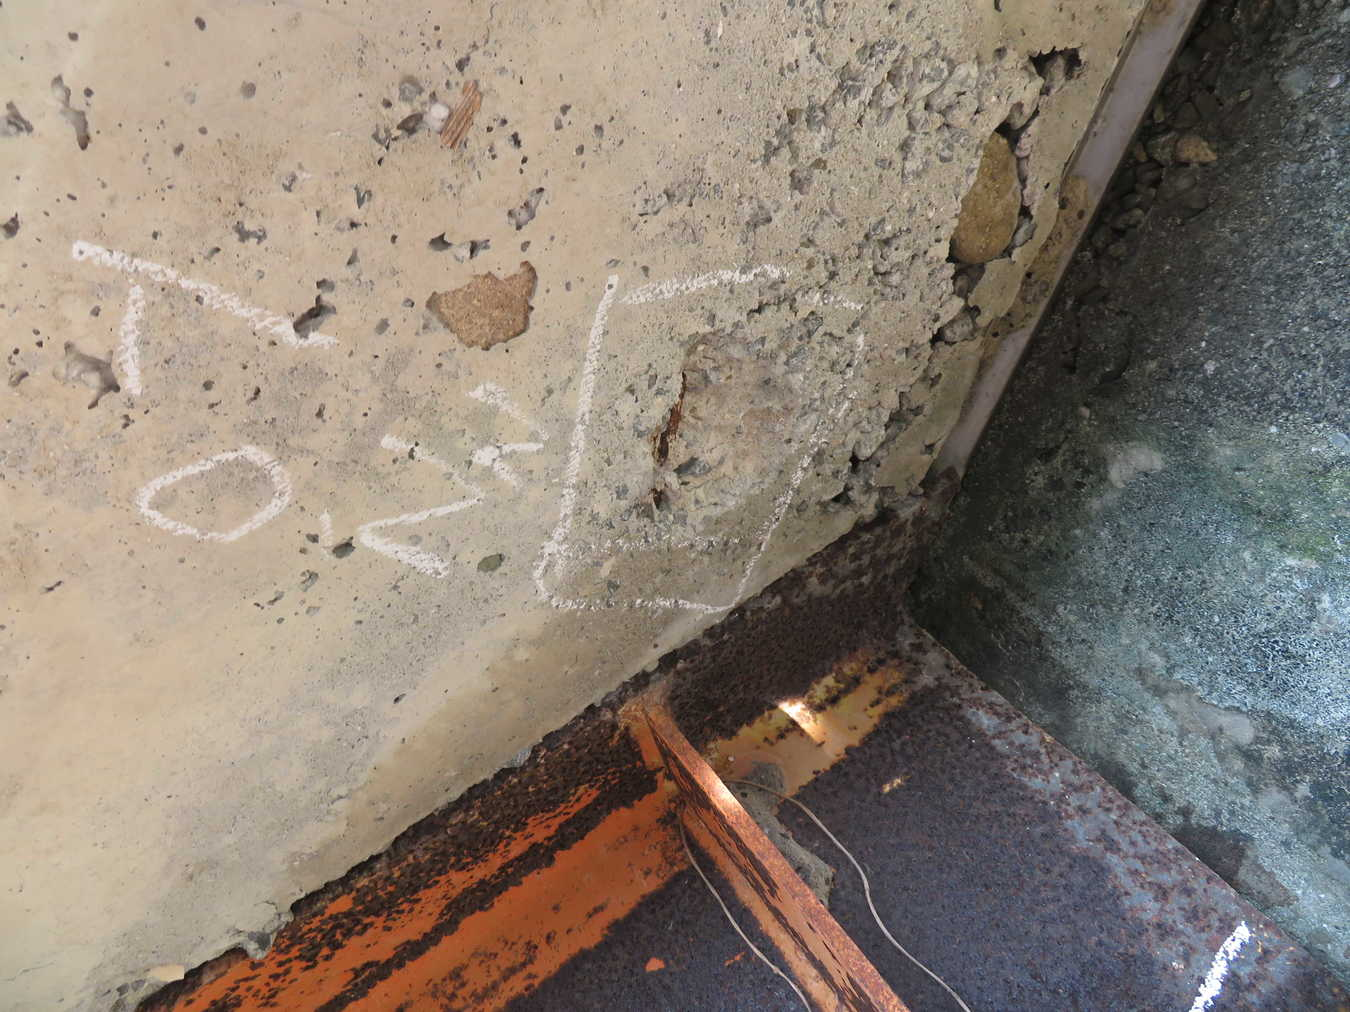
\includegraphics[width=0.675\linewidth]{figures_vlm/s8/s8_07_slab_cracking.jpg}\par}
    \vspace{2pt}
    {\scriptsize\raggedright
    \textbf{Quality Metrics:}~\textit{Sim(emb):~0.806;\enspace Priority:~1.00;\enspace Level:~5}\\[1pt]
    \textbf{GT:} \begin{CJK}{UTF8}{ipxm}・{\CJKfamily{ipxg}床版}に乾燥収縮によるものと推測される{\CJKfamily{ipxg}ひびわれ}、鉄筋の腐食膨張によるものと推測される{\CJKfamily{ipxg}うき}、鉄筋のかぶり不足による{\CJKfamily{ipxg}鉄筋露出}が見られる。また、橋面からの浸透水によるものと推測される{\CJKfamily{ipxg}遊離石灰}が見られる。\end{CJK}\\[1pt]
    \textbf{Pred:} \begin{CJK}{UTF8}{ipxm}主桁に{\CJKfamily{ipxg}ひびわれ}、{\CJKfamily{ipxg}うき}が見られる。また、{\CJKfamily{ipxg}鉄筋露出}もみられる。{\CJKfamily{ipxg}床版}はかぶり不足が原因と思われる{\CJKfamily{ipxg}鉄筋露出}が多数みられる。間詰め部分から錆汁を伴う{\CJKfamily{ipxg}遊離石灰}が見られる。車両通行時には危険性があるため早期措置が望ましい。\end{CJK}
    \par}
  \end{minipage}
  \hfill
  \begin{minipage}[t]{0.46\textwidth}
    {\centering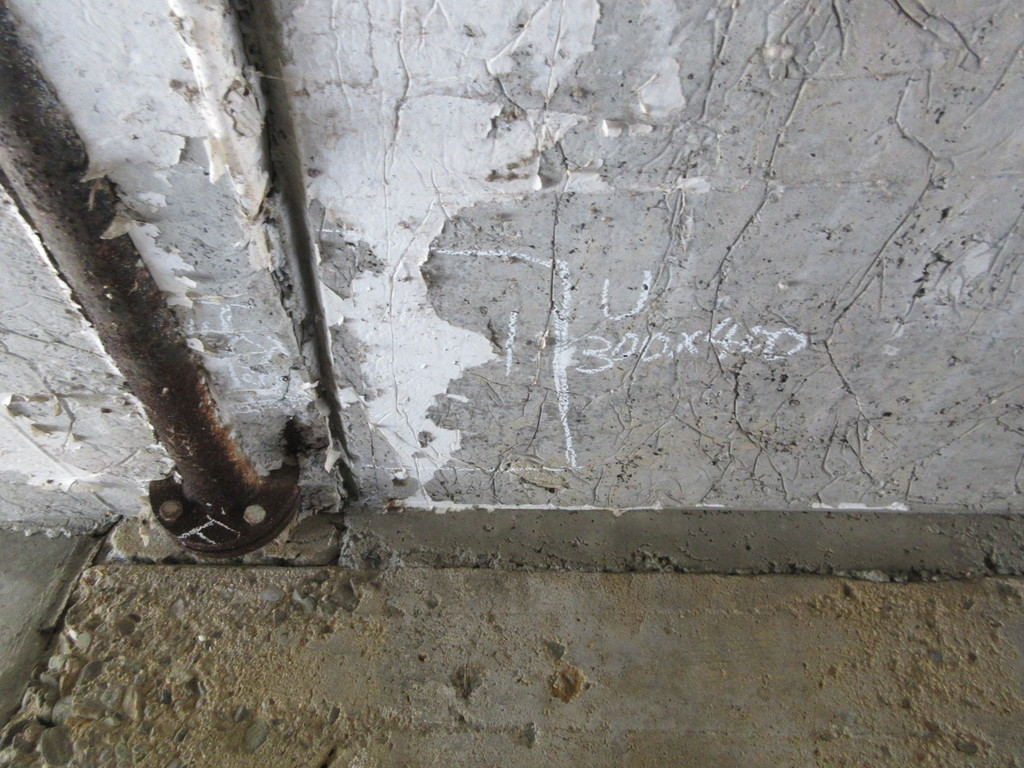
\includegraphics[width=0.675\linewidth]{figures_vlm/s8/s8_08_slab_rebar_exposure.jpg}\par}
    \vspace{2pt}
    {\scriptsize\raggedright
    \textbf{Quality Metrics:}~\textit{Sim(emb):~0.778;\enspace Priority:~0.81;\enspace Level:~4}\\[1pt]
    \textbf{GT:} \begin{CJK}{UTF8}{ipxm}床版に{\CJKfamily{ipxg}うき}、{\CJKfamily{ipxg}鉄筋露出}、{\CJKfamily{ipxg}遊離石灰}が見られる。{\CJKfamily{ipxg}うき}・{\CJKfamily{ipxg}鉄筋露出}は、被り不足や中性化が原因と考えられる。損傷は、局所的であるため、次回点検時に状況の確認を行う。\end{CJK}\\[1pt]
    \textbf{Pred:} \begin{CJK}{UTF8}{ipxm}主桁にひびわれ、{\CJKfamily{ipxg}うき}が見られる。また、{\CJKfamily{ipxg}鉄筋露出}もみられる。間詰め部から{\CJKfamily{ipxg}遊離石灰}（錆汁）が析出している。橋面からの水分の侵入や内部鉄筋の被り不足が原因と思われる。\end{CJK}
    \par}
  \end{minipage}
  \caption{Representative PASS predictions (2/3). \textbf{GT}: pairdata~v3 ground truth (Japanese); \textbf{Pred}: v0.8 LoRA~$r{=}32$ output; \textit{Sim(emb)}: 2048-dim composite cosine similarity; \textit{Priority}: scorer output; \textit{Level}: priority tier.}
  \label{fig:u7_pass_2}
\end{figure}
\clearpage
\begin{figure}[H]
  \centering
  \begin{minipage}[t]{0.46\textwidth}
    {\centering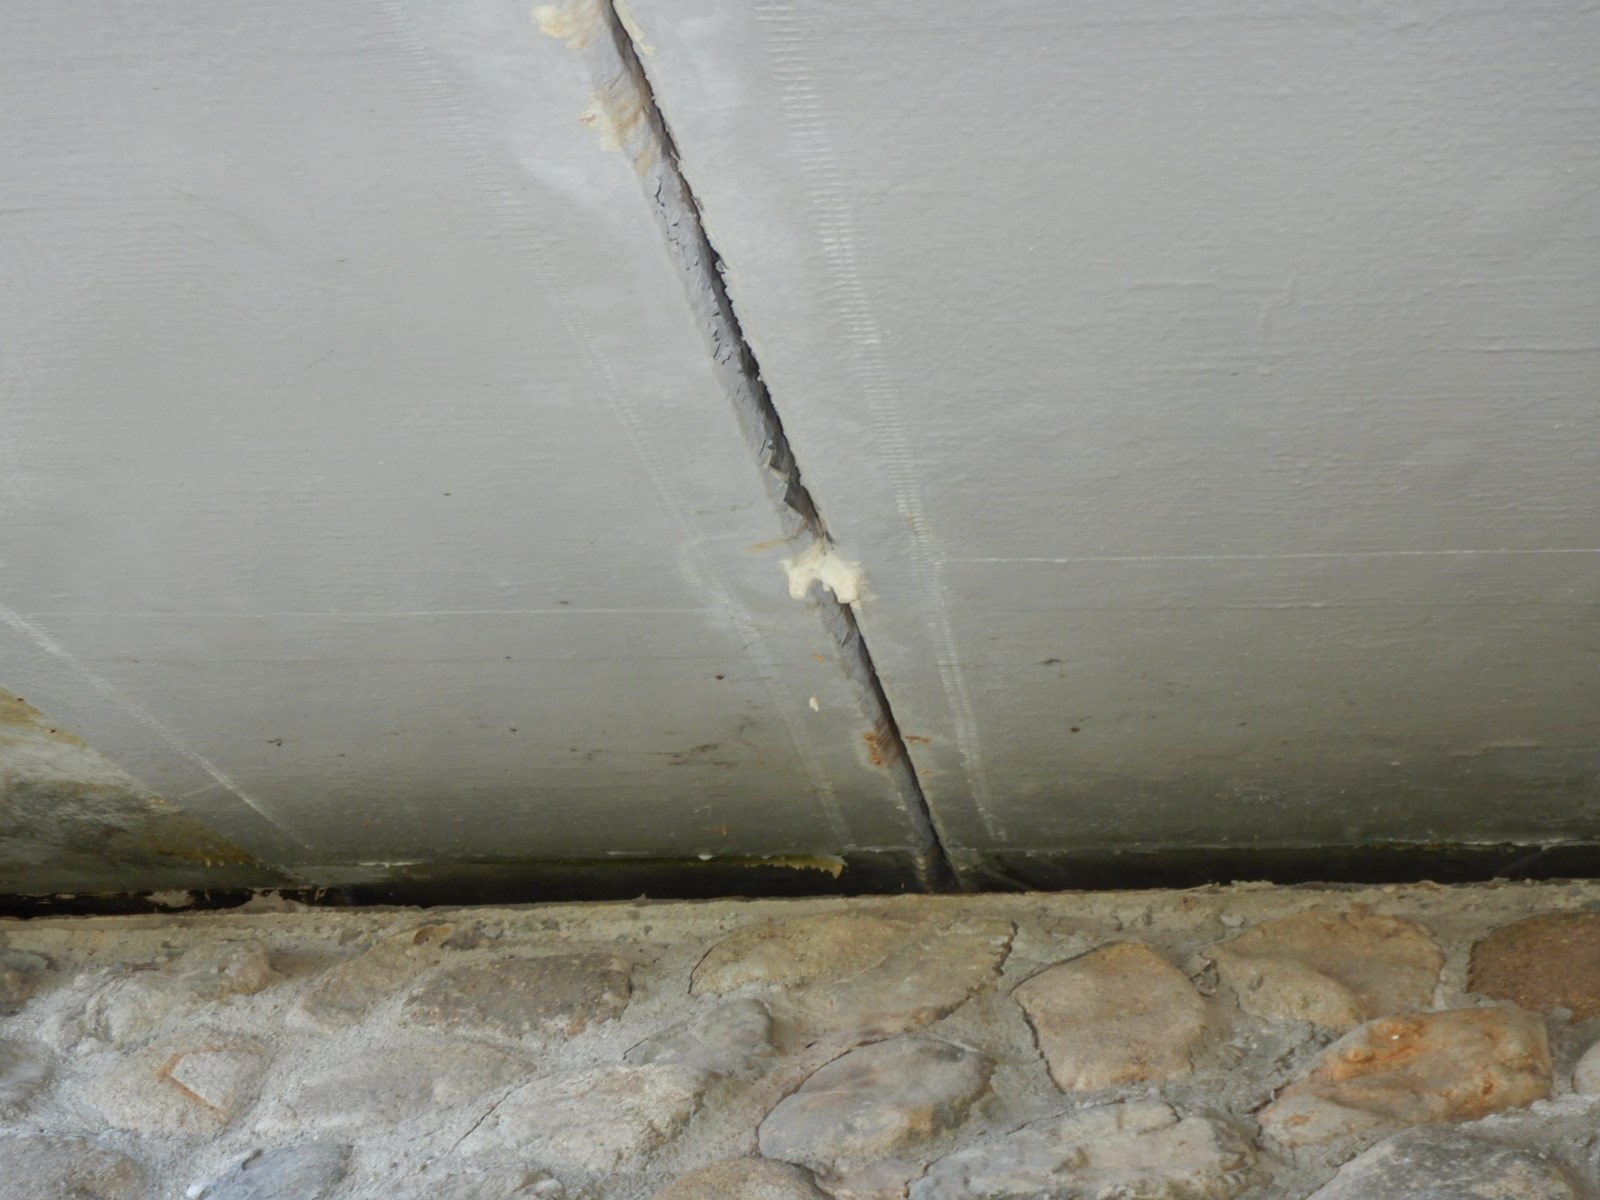
\includegraphics[width=0.675\linewidth]{figures_vlm/s8/s8_09_slab_corrosion.jpg}\par}
    \vspace{2pt}
    {\scriptsize\raggedright
    \textbf{Quality Metrics:}~\textit{Sim(emb):~0.741;\enspace Priority:~0.81;\enspace Level:~4}\\[1pt]
    \textbf{GT:} \begin{CJK}{UTF8}{ipxm}床版間詰め部から{\CJKfamily{ipxg}遊離石灰}（{\CJKfamily{ipxg}錆}汁）が見られる。損傷は状況に応じて補修を行う事が望ましい。\end{CJK}\\[1pt]
    \textbf{Pred:} \begin{CJK}{UTF8}{ipxm}主桁にひびわれ、うきが見られる。また、鉄筋露出もみられる。間詰め部から{\CJKfamily{ipxg}遊離石灰}（{\CJKfamily{ipxg}錆}汁）が析出している。橋面からの水分の侵入や地覆からの伝い水等が原因と思われる。\end{CJK}
    \par}
  \end{minipage}
  \hfill
  \begin{minipage}[t]{0.46\textwidth}
    {\centering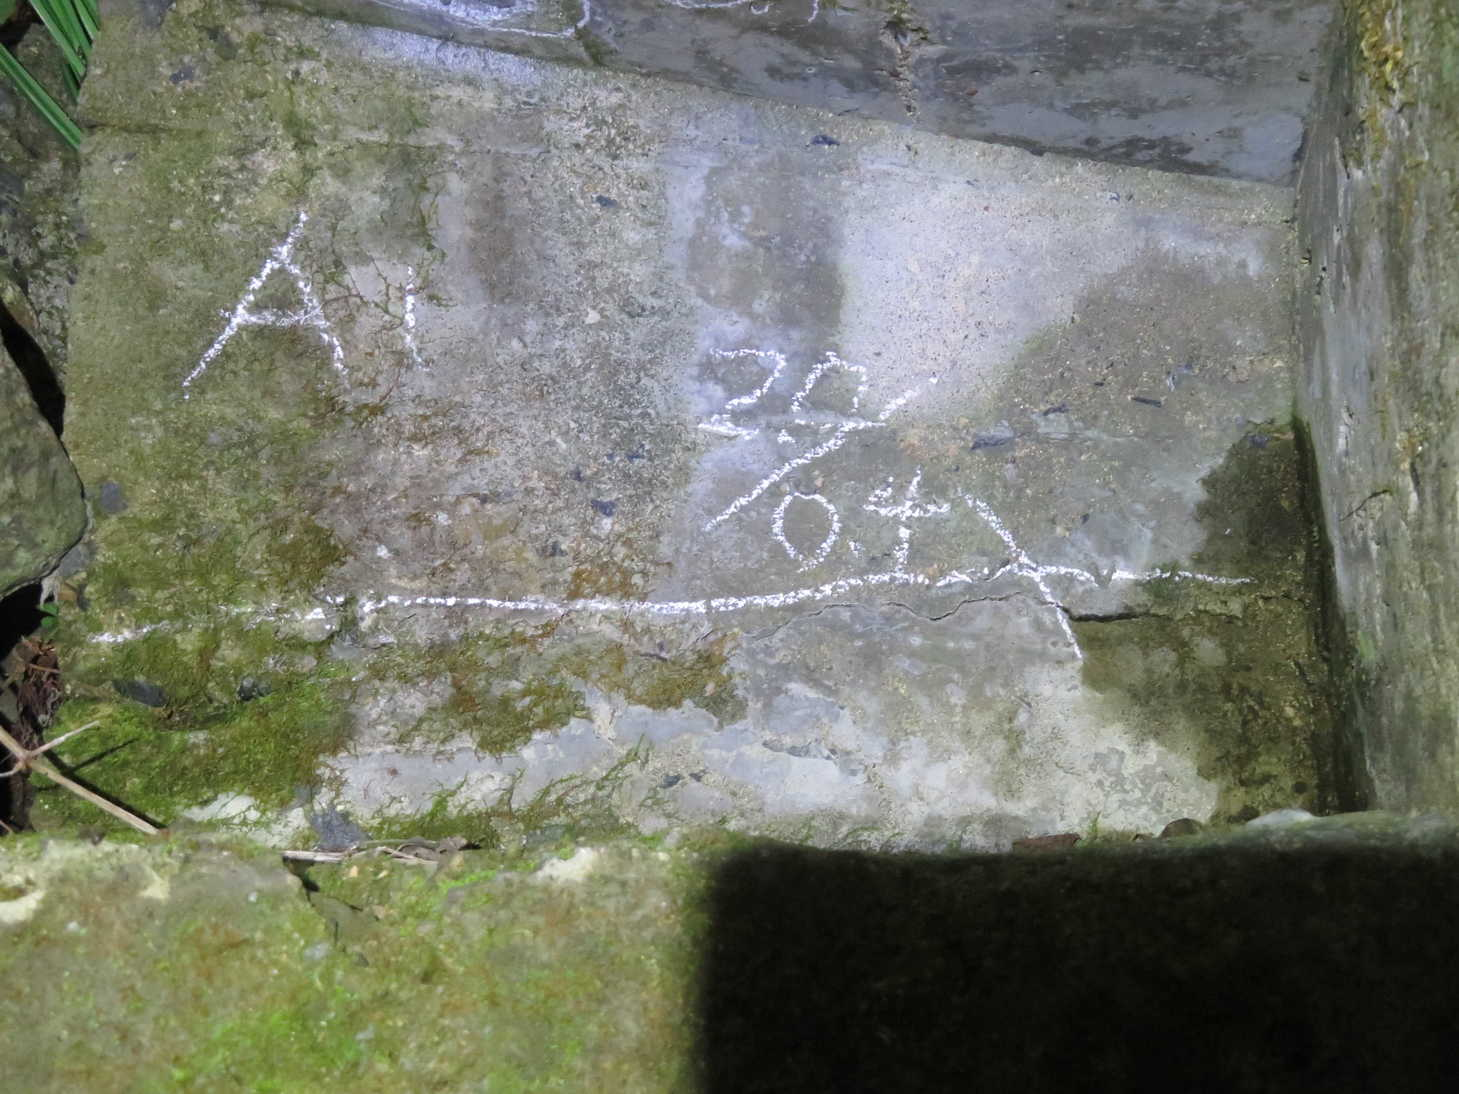
\includegraphics[width=0.675\linewidth]{figures_vlm/s8/s8_10_abutment_cracking.jpg}\par}
    \vspace{2pt}
    {\scriptsize\raggedright
    \textbf{Quality Metrics:}~\textit{Sim(emb):~0.798;\enspace Priority:~1.00;\enspace Level:~5}\\[1pt]
    \textbf{GT:} \begin{CJK}{UTF8}{ipxm}・橋台に施工不良による{\CJKfamily{ipxg}ひびわれ}（コールドジョイント）および鉄筋のかぶり不足による{\CJKfamily{ipxg}鉄筋露出}が見られる。また、伸縮装置部からの{\CJKfamily{ipxg}漏水}による{\CJKfamily{ipxg}漏水}跡およびすりへりが見られる。\end{CJK}\\[1pt]
    \textbf{Pred:} \begin{CJK}{UTF8}{ipxm}主桁に{\CJKfamily{ipxg}ひびわれ}、うきが見られる。また、{\CJKfamily{ipxg}鉄筋露出}もみられる。床版はかぶり不足が原因と思われる{\CJKfamily{ipxg}鉄筋露出}が多数みられる。間詰め部分から錆汁を伴う{\CJKfamily{ipxg}漏水}跡が見られる。防護柵に変形が見られる。\end{CJK}
    \par}
  \end{minipage}
  \\[4pt]
  \begin{minipage}[t]{0.46\textwidth}
    {\centering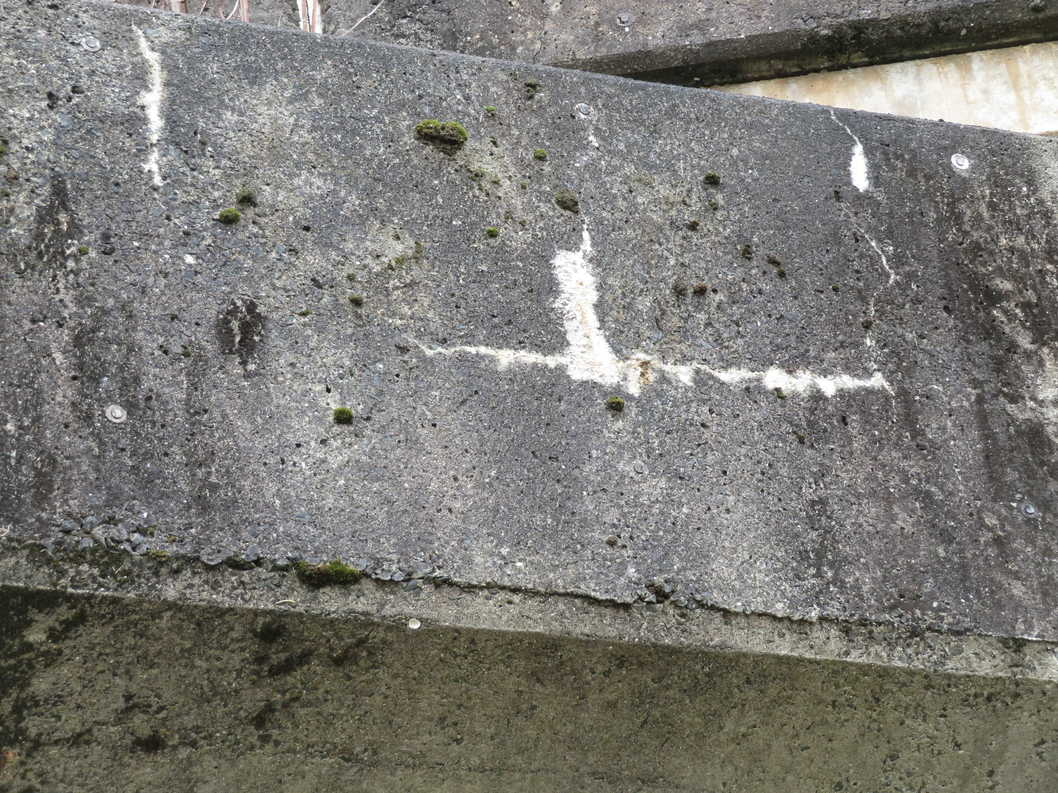
\includegraphics[width=0.675\linewidth]{figures_vlm/s8/s8_11_abutment_rebar_exposure.jpg}\par}
    \vspace{2pt}
    {\scriptsize\raggedright
    \textbf{Quality Metrics:}~\textit{Sim(emb):~0.797;\enspace Priority:~0.81;\enspace Level:~4}\\[1pt]
    \textbf{GT:} \begin{CJK}{UTF8}{ipxm}・橋脚に鉄筋の腐食膨張によるものと推測される{\CJKfamily{ipxg}うき}および鉄筋のかぶり不足による{\CJKfamily{ipxg}鉄筋露出}がみられる。また、橋面からの浸透水によるものと推測される軽微{\CJKfamily{ipxg}遊離石灰}が見られる。・橋台に伸縮装置部からの漏水による漏水跡が見られる。\end{CJK}\\[1pt]
    \textbf{Pred:} \begin{CJK}{UTF8}{ipxm}主桁にひびわれ、{\CJKfamily{ipxg}うき}が見られる。また、{\CJKfamily{ipxg}鉄筋露出}もみられる。間詰め部から{\CJKfamily{ipxg}遊離石灰}（錆汁）が見られる。橋面からの水分の侵入や地覆からの伝い水等が原因と思われる。\end{CJK}
    \par}
  \end{minipage}
  \hfill
  \begin{minipage}[t]{0.46\textwidth}
    {\centering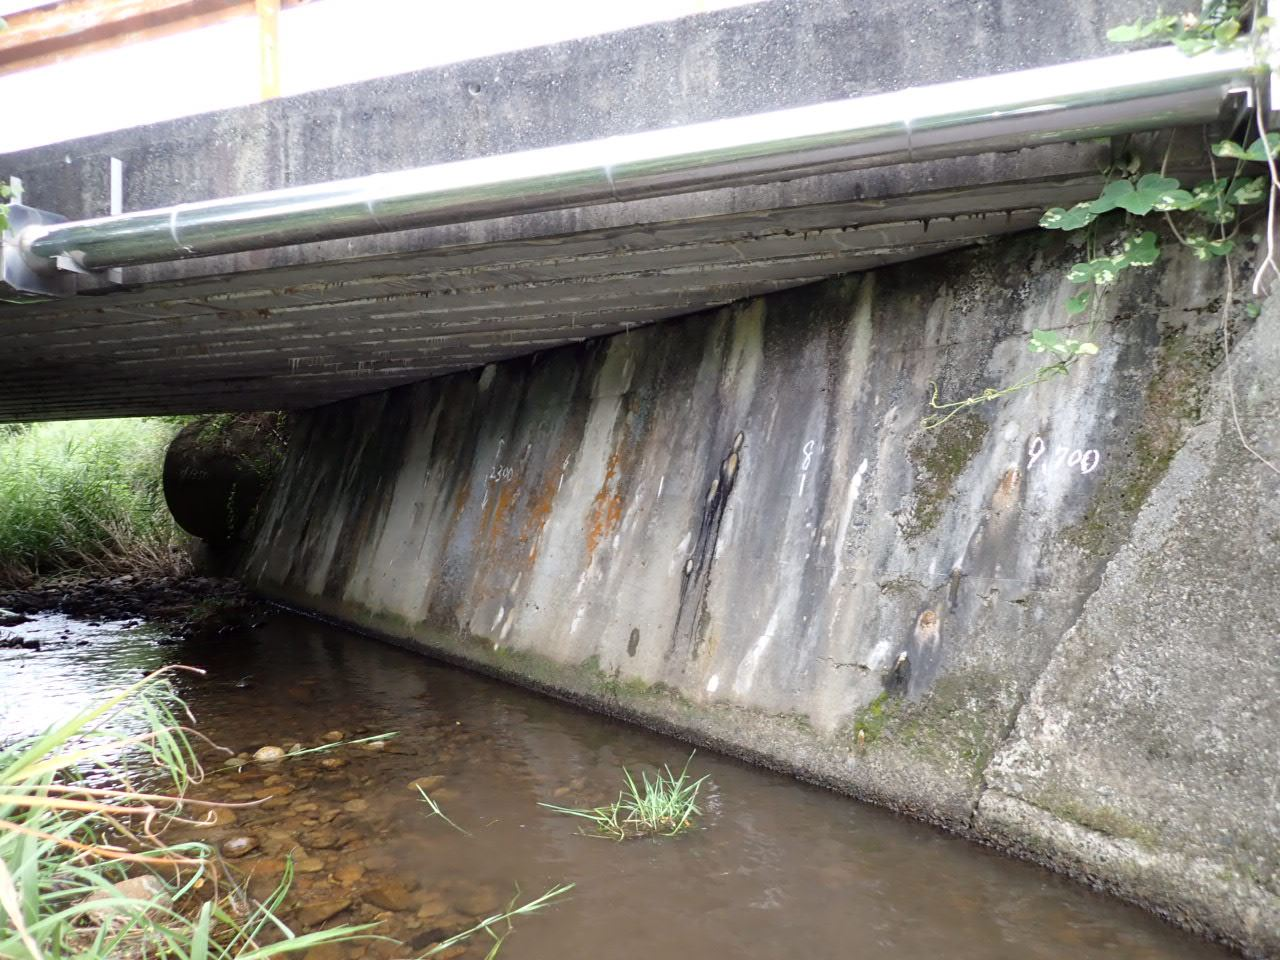
\includegraphics[width=0.675\linewidth]{figures_vlm/s8/s8_12_abutment_spalling.jpg}\par}
    \vspace{2pt}
    {\scriptsize\raggedright
    \textbf{Quality Metrics:}~\textit{Sim(emb):~0.669;\enspace Priority:~0.81;\enspace Level:~4}\\[1pt]
    \textbf{GT:} \begin{CJK}{UTF8}{ipxm}橋台に{\CJKfamily{ipxg}うき}、{\CJKfamily{ipxg}漏水}がみられる。{\CJKfamily{ipxg}漏水}は伸縮装置から浸入したものと考えられる。緊急性はなく、予防保全の観点から健全度評価「Ⅱ」とする。\end{CJK}\\[1pt]
    \textbf{Pred:} \begin{CJK}{UTF8}{ipxm}主桁にひびわれ、{\CJKfamily{ipxg}うき}が見られる。また、鉄筋露出もみられる。間詰め部から錆汁を伴う{\CJKfamily{ipxg}漏水}が生じており、それによって内部鉄筋が著しく腐食している。床版は健全である。道路橋の機能に支障が生じていないため、次回点検時に状況の確認を行うことが望ましい。\end{CJK}
    \par}
  \end{minipage}
  \caption{Representative PASS predictions (3/3). \textbf{GT}: pairdata~v3 ground truth (Japanese); \textbf{Pred}: v0.8 LoRA~$r{=}32$ output; \textit{Sim(emb)}: 2048-dim composite cosine similarity; \textit{Priority}: scorer output; \textit{Level}: priority tier.}
  \label{fig:u7_pass_3}
\end{figure}
\clearpage

%%--------------------------------------------------------------------
\clearpage
%%--------------------------------------------------------------------
\clearpage
\subsection*{U.7.1\quad DoRA $r{=}32$ vs.\ LoRA $r{=}32$: Same-Image Comparison}
\label{sec:u71}
%%--------------------------------------------------------------------

Figures~\ref{fig:u71_comp_1}--\ref{fig:u71_comp_3} show the same twelve images
used in U.7, now captioned with predictions from both the LoRA~$r{=}32$ model
(v0.8) and the DoRA~$r{=}32$ model (v0.9).
\textit{Sim(emb)} values are listed separately for each model to allow
direct comparison of embedding-level quality.
Bold text indicates keywords appearing in both the ground truth and the
respective model output.

\begin{figure}[H]
  \centering
  \begin{minipage}[t]{0.46\textwidth}
    {\centering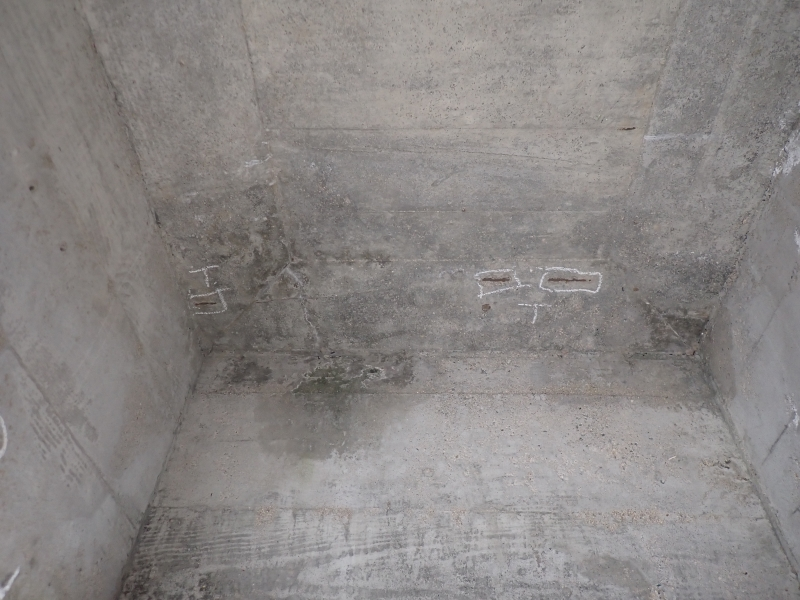
\includegraphics[width=0.675\linewidth]{figures_vlm/s8/s8_01_girder_cracking.jpg}\par}
    \vspace{2pt}
    {\scriptsize\raggedright
    \textbf{LoRA~$r{=}32$:}~\textit{Sim(emb):~0.840;\enspace Priority:~1.00;\enspace Level:~5}\\[1pt]
    \textbf{DoRA~$r{=}32$:}~\textit{Sim(emb):~0.766;\enspace Priority:~0.81;\enspace Level:~4}\\[1pt]
    \textbf{GT:} \begin{CJK}{UTF8}{ipxm}{\CJKfamily{ipxg}主桁}に{\CJKfamily{ipxg}ひびわれ}（最大W=0.3mm)・{\CJKfamily{ipxg}鉄筋露出}・{\CJKfamily{ipxg}うき}・{\CJKfamily{ipxg}遊離石灰}・漏水跡、{\CJKfamily{ipxg}床版}に{\CJKfamily{ipxg}鉄筋露出}・破損・剥離・{\CJKfamily{ipxg}遊離石灰}が見られる。{\CJKfamily{ipxg}主桁}の損傷は、鉄筋の被り不足及び中性化・コンクリートの低品質、{\CJKfamily{ipxg}床版}の損傷は、鉄筋の被り不足・防護柵の施工が原因と考えられる。前回点検から{\CJKfamily{ipxg}鉄筋露出}に進展が見られるため、経過観察を行い、状況により補修を行う。\end{CJK}\\[1pt]
    \textbf{LoRA Pred:} \begin{CJK}{UTF8}{ipxm}{\CJKfamily{ipxg}主桁}に{\CJKfamily{ipxg}ひびわれ}、{\CJKfamily{ipxg}うき}が見られる。また、{\CJKfamily{ipxg}鉄筋露出}もみられる。{\CJKfamily{ipxg}床版}はかぶり不足が原因と思われる{\CJKfamily{ipxg}鉄筋露出}が多数みられる。間詰め部分から錆汁を伴う{\CJKfamily{ipxg}遊離石灰}が見られる。車両通行時には危険性があるため早期措置が望ましい。\end{CJK}\\[1pt]
    \textbf{DoRA Pred:} \begin{CJK}{UTF8}{ipxm}{\CJKfamily{ipxg}主桁}に{\CJKfamily{ipxg}ひびわれ}、{\CJKfamily{ipxg}鉄筋露出}が見られる。また、PC{\CJKfamily{ipxg}床版}部からの{\CJKfamily{ipxg}遊離石灰}もみられる。車両通行時の視線や近づきは限定的であるが、必要に応じて断面修理等が望ましい。\end{CJK}
    \par}
  \end{minipage}
  \hfill
  \begin{minipage}[t]{0.46\textwidth}
    {\centering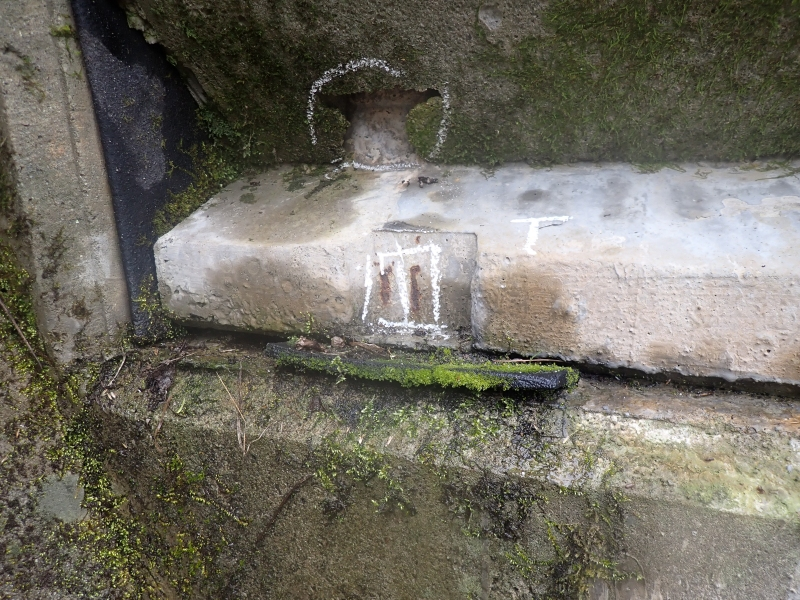
\includegraphics[width=0.675\linewidth]{figures_vlm/s8/s8_02_girder_rebar_exposure.jpg}\par}
    \vspace{2pt}
    {\scriptsize\raggedright
    \textbf{LoRA~$r{=}32$:}~\textit{Sim(emb):~0.808;\enspace Priority:~0.81;\enspace Level:~4}\\[1pt]
    \textbf{DoRA~$r{=}32$:}~\textit{Sim(emb):~0.659;\enspace Priority:~0.81;\enspace Level:~4}\\[1pt]
    \textbf{GT:} \begin{CJK}{UTF8}{ipxm}{\CJKfamily{ipxg}主桁}に{\CJKfamily{ipxg}鉄筋露出}、間詰めに漏水・{\CJKfamily{ipxg}遊離石灰}が見られる。{\CJKfamily{ipxg}主桁}の{\CJKfamily{ipxg}鉄筋露出}は被り不足、間詰めの損傷は、橋面からの漏水が原因と考えられる。{\CJKfamily{ipxg}主桁}の損傷は前回確認されていないが局所的である。道路橋の機能に支障は生じていないため、次回点検時に状況の確認を行う。\end{CJK}\\[1pt]
    \textbf{LoRA Pred:} \begin{CJK}{UTF8}{ipxm}{\CJKfamily{ipxg}主桁}にひびわれ、うきが見られる。また、{\CJKfamily{ipxg}鉄筋露出}もみられる。間詰め部から{\CJKfamily{ipxg}遊離石灰}（錆汁）が析出している。橋面からの水分の侵入や地覆からの伝い水等が原因と思われる。局所的である為，経過観察とする。\end{CJK}\\[1pt]
    \textbf{DoRA Pred:} \begin{CJK}{UTF8}{ipxm}{\CJKfamily{ipxg}主桁}にひびわれ、うきが見られる。また、{\CJKfamily{ipxg}鉄筋露出}もみられる。床版に一方向ひびわれが見られる。車両通行時の視線や近づけない高所からの人工除去等であれば影響は限定的であり、経過観察とする。\end{CJK}
    \par}
  \end{minipage}
  \\[4pt]
  \begin{minipage}[t]{0.46\textwidth}
    {\centering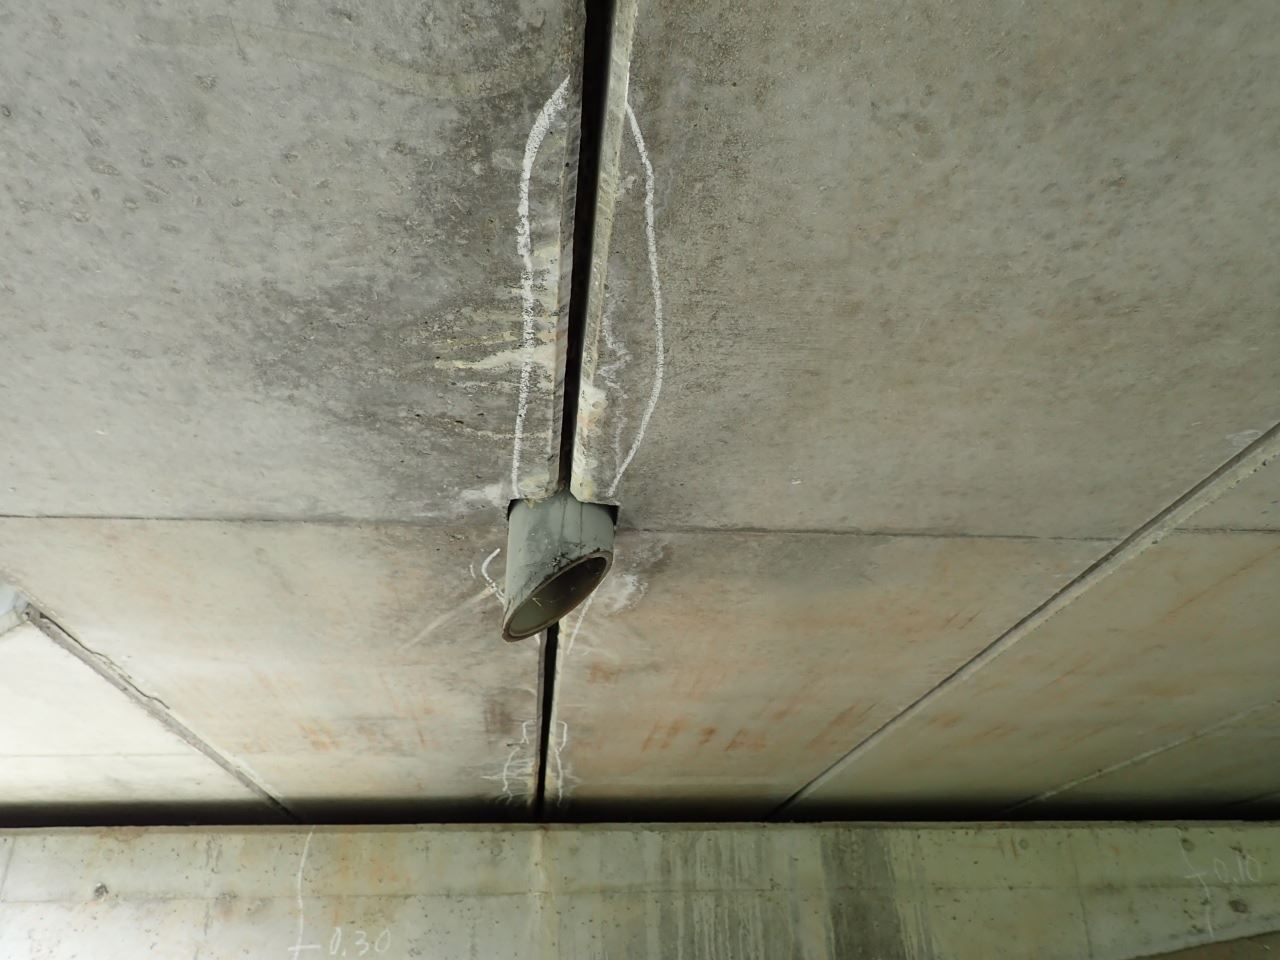
\includegraphics[width=0.675\linewidth]{figures_vlm/s8/s8_03_girder_spalling.jpg}\par}
    \vspace{2pt}
    {\scriptsize\raggedright
    \textbf{LoRA~$r{=}32$:}~\textit{Sim(emb):~0.774;\enspace Priority:~0.81;\enspace Level:~4}\\[1pt]
    \textbf{DoRA~$r{=}32$:}~\textit{Sim(emb):~0.612;\enspace Priority:~0.81;\enspace Level:~4}\\[1pt]
    \textbf{GT:} \begin{CJK}{UTF8}{ipxm}{\CJKfamily{ipxg}主桁}に後埋めモルタルの剥離・鋼材露出、間詰めに一部{\CJKfamily{ipxg}錆}汁を伴う{\CJKfamily{ipxg}遊離石灰}が見られる。経過観察を行い、状況により補修を行う。\end{CJK}\\[1pt]
    \textbf{LoRA Pred:} \begin{CJK}{UTF8}{ipxm}{\CJKfamily{ipxg}主桁}にひびわれ、うきが見られる。また、鉄筋露出もみられる。間詰め部から{\CJKfamily{ipxg}遊離石灰}（{\CJKfamily{ipxg}錆}汁）が析出している。添加物の目地板に表面的な腐食が見られる。\end{CJK}\\[1pt]
    \textbf{DoRA Pred:} \begin{CJK}{UTF8}{ipxm}{\CJKfamily{ipxg}主桁}にひびわれ、うきが見られる。また、鉄筋露出もみられる。車両通行時の視線や近づけない高所からの人工修理等では、直接的な影響はあるが、本格的な復旧後の保全機能を果たす必要がある。\end{CJK}
    \par}
  \end{minipage}
  \hfill
  \begin{minipage}[t]{0.46\textwidth}
    {\centering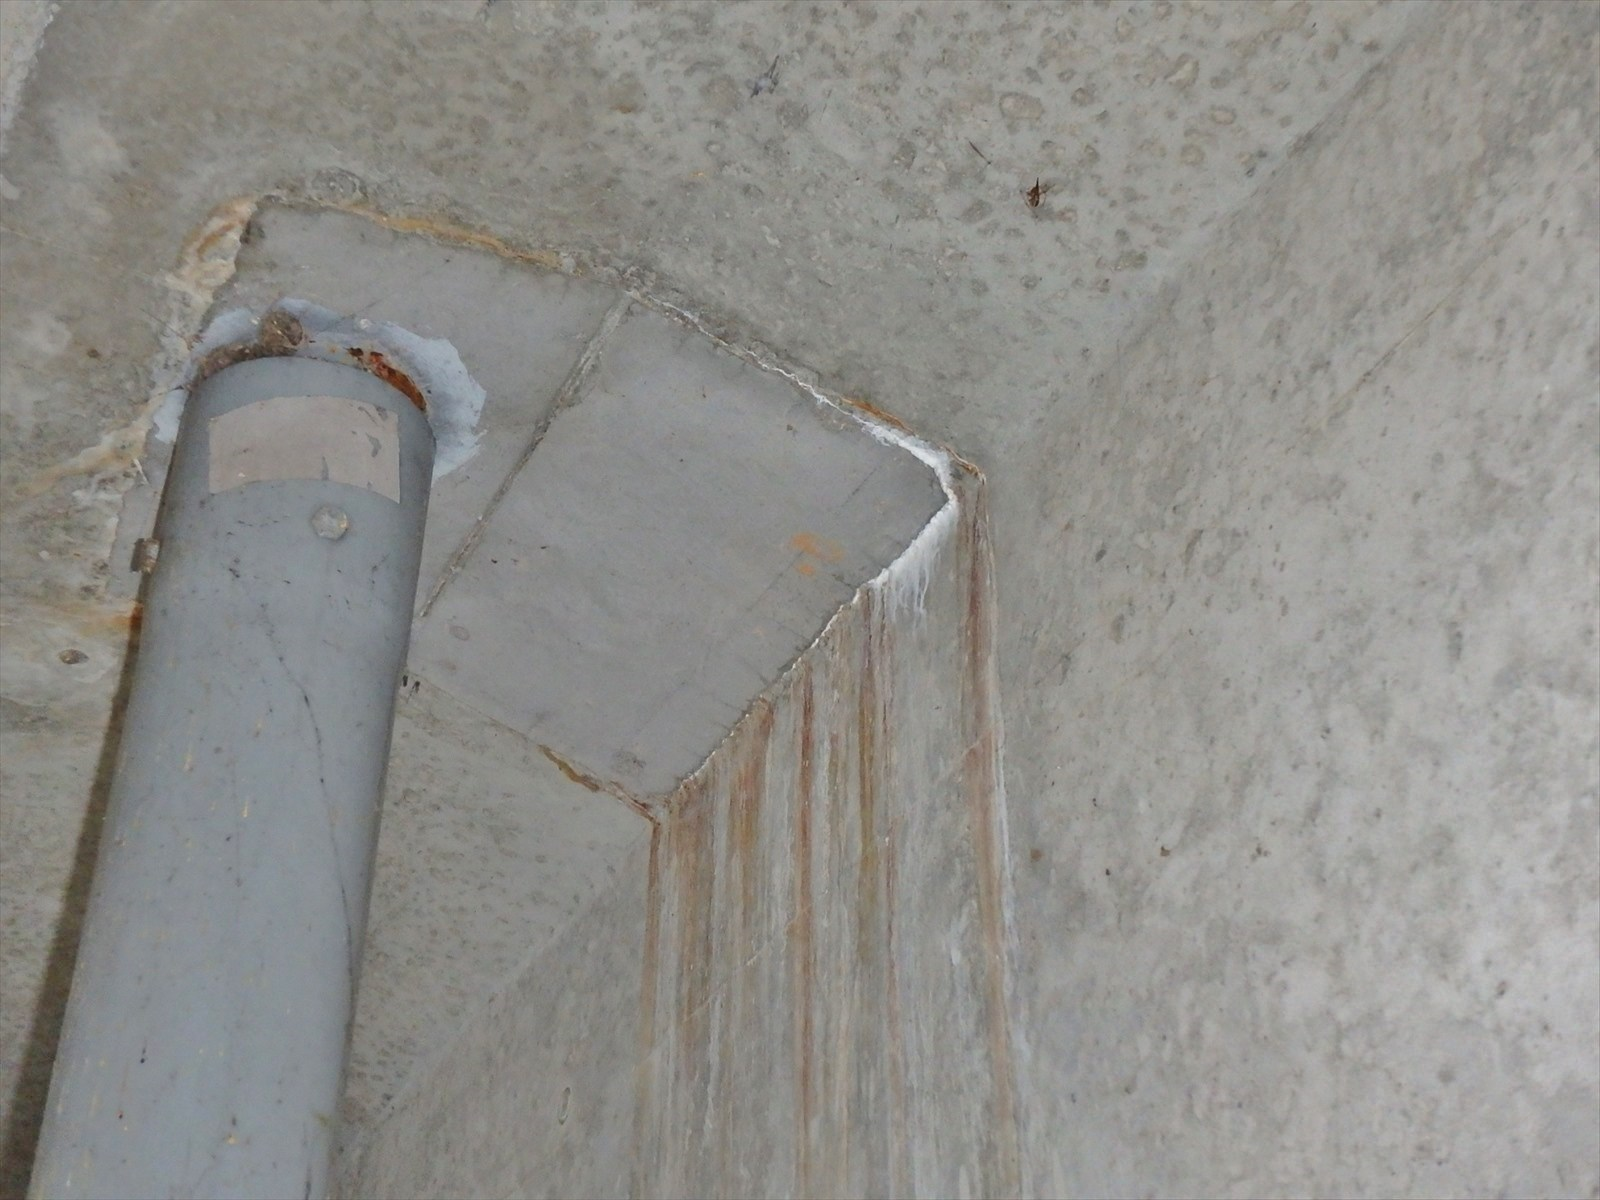
\includegraphics[width=0.675\linewidth]{figures_vlm/s8/s8_04_girder_corrosion.jpg}\par}
    \vspace{2pt}
    {\scriptsize\raggedright
    \textbf{LoRA~$r{=}32$:}~\textit{Sim(emb):~0.713;\enspace Priority:~0.81;\enspace Level:~4}\\[1pt]
    \textbf{DoRA~$r{=}32$:}~\textit{Sim(emb):~0.615;\enspace Priority:~0.81;\enspace Level:~4}\\[1pt]
    \textbf{GT:} \begin{CJK}{UTF8}{ipxm}{\CJKfamily{ipxg}主桁}に漏水跡（{\CJKfamily{ipxg}錆}汁）が見られる。損傷は状況に応じて補修を行う事が望ましい。\end{CJK}\\[1pt]
    \textbf{LoRA Pred:} \begin{CJK}{UTF8}{ipxm}{\CJKfamily{ipxg}主桁}にひびわれ、うきが見られる。また、鉄筋露出もみられる。間詰め部から遊離石灰（{\CJKfamily{ipxg}錆}汁）が析出している。橋面からの水分の侵入や地覆からの伝い水等が原因と思われる。\end{CJK}\\[1pt]
    \textbf{DoRA Pred:} \begin{CJK}{UTF8}{ipxm}{\CJKfamily{ipxg}主桁}にひびわれ、うきが見られる。また、鉄筋露出もみられる。床版に一方向ひびわれが見られる。車両通行時の視線や近づけない高所からの人工除去等であれば影響は限定的であり、経過観察とする。\end{CJK}
    \par}
  \end{minipage}
  \caption{LoRA $r{=}32$ vs.\ DoRA $r{=}32$ on the same twelve images (1/3). \textbf{GT}: ground truth; \textbf{LoRA/DoRA Pred}: respective model outputs; \textit{Sim(emb)}: 2048-dim composite cosine similarity; \textit{Priority}/\textit{Level}: scorer output / priority tier.}
  \label{fig:u71_comp_1}
\end{figure}
\clearpage
\begin{figure}[H]
  \centering
  \begin{minipage}[t]{0.46\textwidth}
    {\centering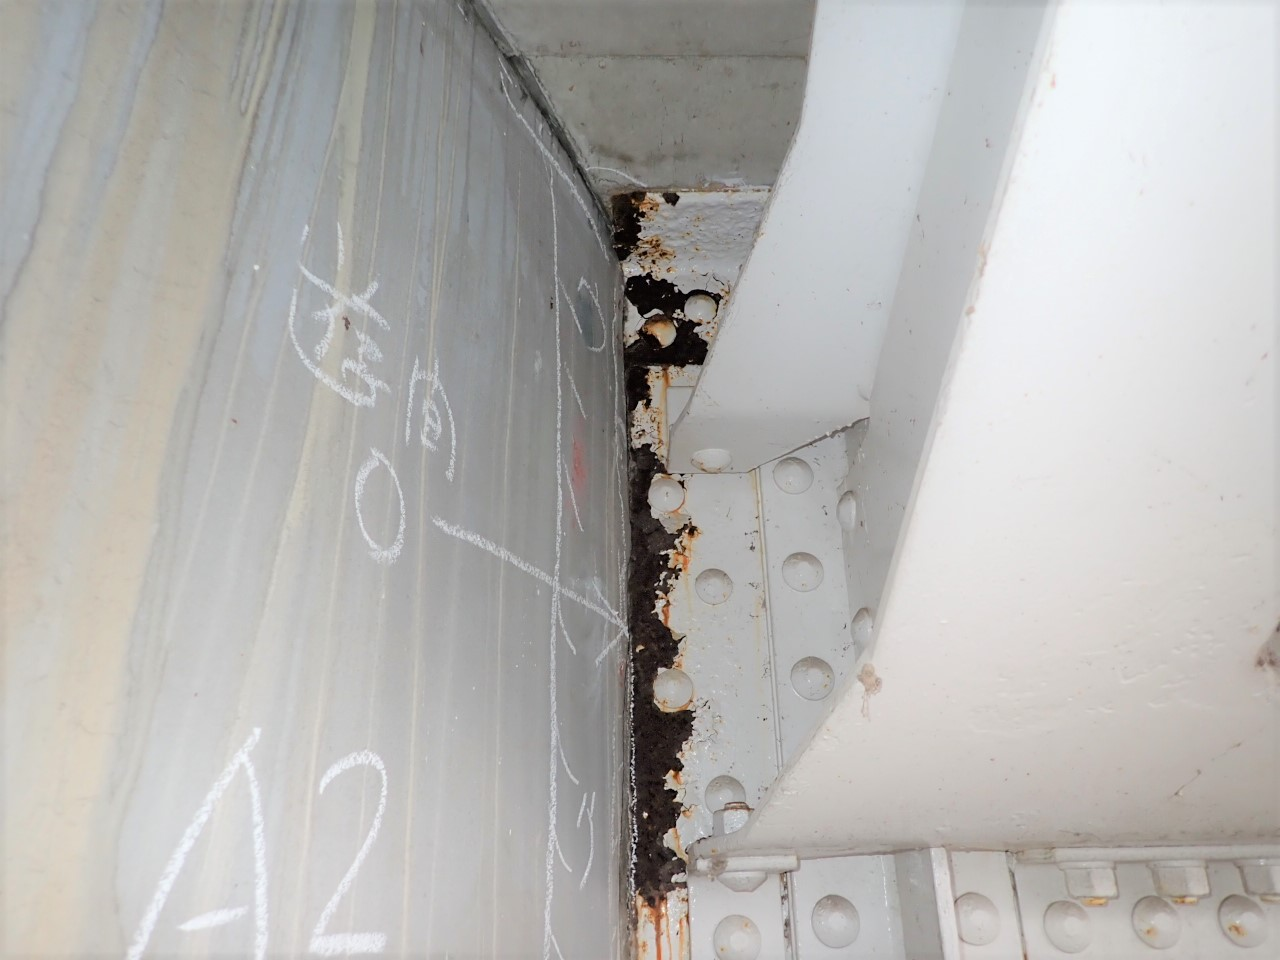
\includegraphics[width=0.675\linewidth]{figures_vlm/s8/s8_05_girder_settlement.jpg}\par}
    \vspace{2pt}
    {\scriptsize\raggedright
    \textbf{LoRA~$r{=}32$:}~\textit{Sim(emb):~0.572;\enspace Priority:~0.81;\enspace Level:~4}\\[1pt]
    \textbf{DoRA~$r{=}32$:}~\textit{Sim(emb):~0.589;\enspace Priority:~0.81;\enspace Level:~4}\\[1pt]
    \textbf{GT:} \begin{CJK}{UTF8}{ipxm}伸縮装置にゴムの変形、A2橋台パラペットと{\CJKfamily{ipxg}主桁}の接触が見られる。経過観察を行い、状況により補修を行う。\end{CJK}\\[1pt]
    \textbf{LoRA Pred:} \begin{CJK}{UTF8}{ipxm}{\CJKfamily{ipxg}主桁}にひびわれ、うきが見られる。また、鉄筋露出もみられる。間詰め部から遊離石灰（錆汁）が析出している。橋面からの水分の侵入や地覆からの伝い水等が原因と思われる。\end{CJK}\\[1pt]
    \textbf{DoRA Pred:} \begin{CJK}{UTF8}{ipxm}{\CJKfamily{ipxg}主桁}にひびわれ、うきが見られる。また、鉄筋露出もみられる。車両通行時はなかったが、高水位時や洗流等により、道路橋が被り不足していた場合は、土砂流入により支承・ボルトが覆われる可能性がある。今後進めて必要であれば、止水機能向上（目地）と、河川管理にて速やかに対策を行うことが望ましい。\end{CJK}
    \par}
  \end{minipage}
  \hfill
  \begin{minipage}[t]{0.46\textwidth}
    {\centering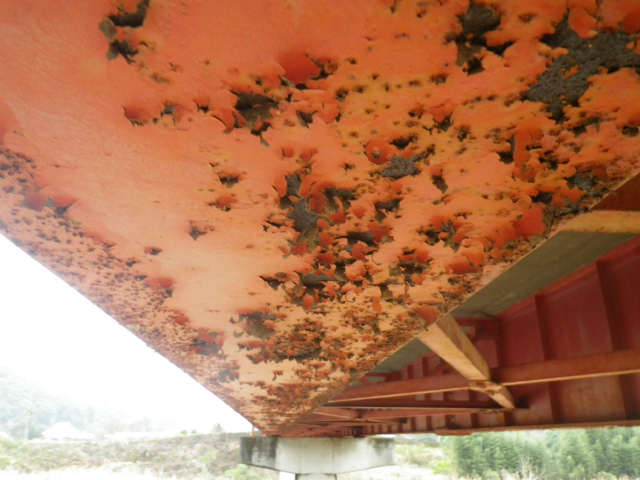
\includegraphics[width=0.675\linewidth]{figures_vlm/s8/s8_06_girder_other.jpg}\par}
    \vspace{2pt}
    {\scriptsize\raggedright
    \textbf{LoRA~$r{=}32$:}~\textit{Sim(emb):~0.585;\enspace Priority:~0.81;\enspace Level:~4}\\[1pt]
    \textbf{DoRA~$r{=}32$:}~\textit{Sim(emb):~0.546;\enspace Priority:~0.81;\enspace Level:~4}\\[1pt]
    \textbf{GT:} \begin{CJK}{UTF8}{ipxm}{\CJKfamily{ipxg}主桁}・横桁に塗装剥がれや防食機能の劣化が認められる\end{CJK}\\[1pt]
    \textbf{LoRA Pred:} \begin{CJK}{UTF8}{ipxm}{\CJKfamily{ipxg}主桁}にひびわれ、うきが見られる。また、鉄筋露出もみられる。間詰め部から遊離石灰（錆汁）が析出している。橋面からの水分の侵入や地覆からの伝い水等が原因と思われる。高力ボルト・ナットは使用中であり、今後継目材の変更等によって止水機能の向上を行う必要がある。\end{CJK}\\[1pt]
    \textbf{DoRA Pred:} \begin{CJK}{UTF8}{ipxm}{\CJKfamily{ipxg}主桁}にひびわれ、うきが見られる。また、鉄筋露出もみられる。上部ハンチにかぶり不足および伝え水が原因と思われる。PC床版は健全である。\end{CJK}
    \par}
  \end{minipage}
  \\[4pt]
  \begin{minipage}[t]{0.46\textwidth}
    {\centering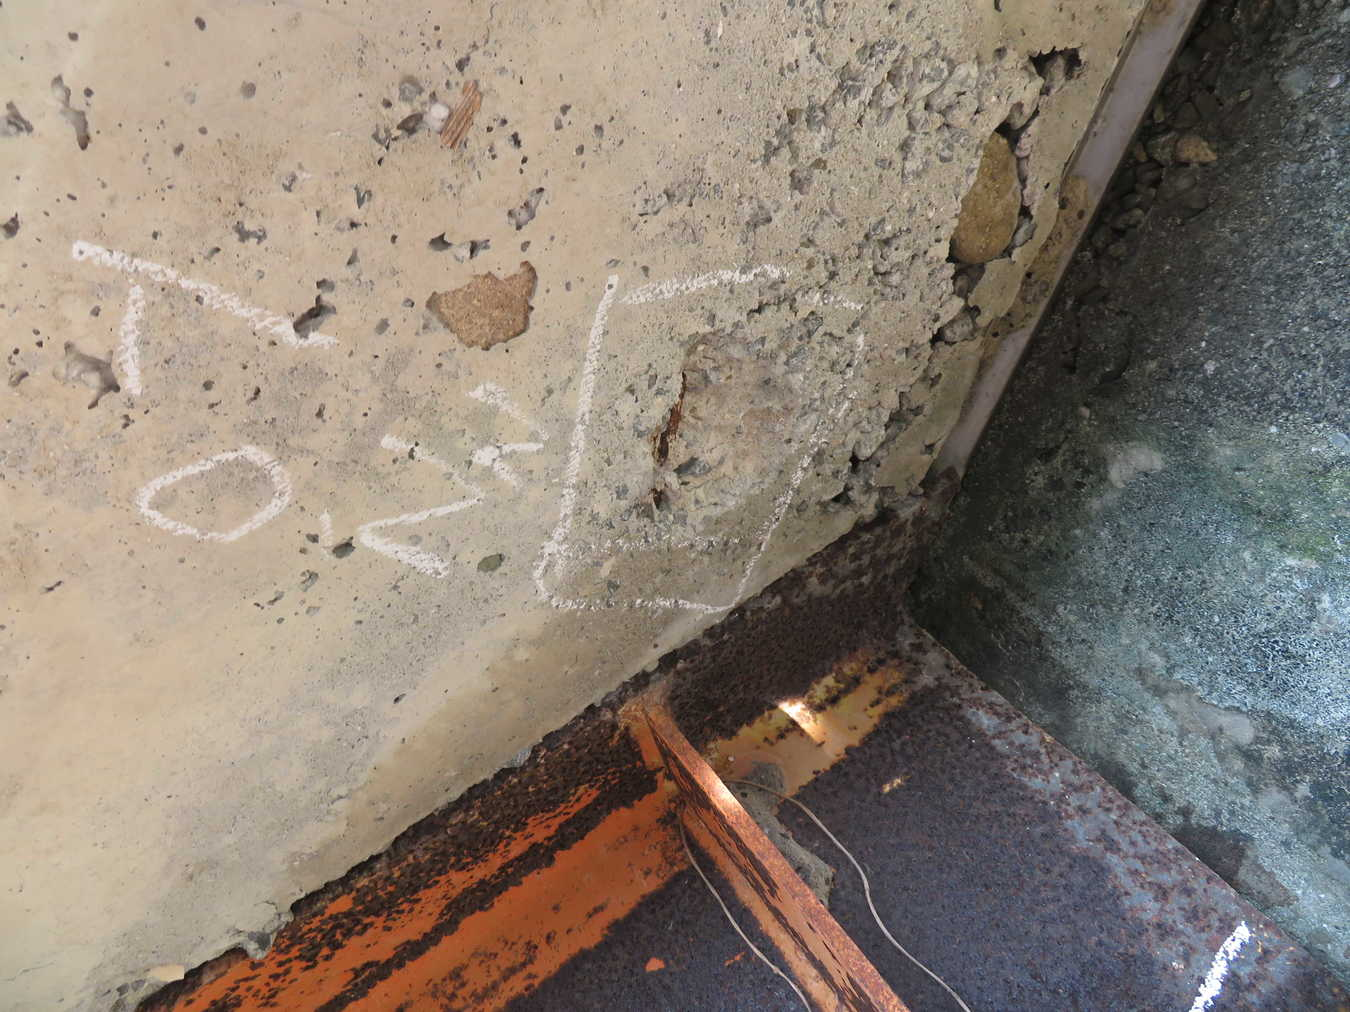
\includegraphics[width=0.675\linewidth]{figures_vlm/s8/s8_07_slab_cracking.jpg}\par}
    \vspace{2pt}
    {\scriptsize\raggedright
    \textbf{LoRA~$r{=}32$:}~\textit{Sim(emb):~0.806;\enspace Priority:~1.00;\enspace Level:~5}\\[1pt]
    \textbf{DoRA~$r{=}32$:}~\textit{Sim(emb):~0.778;\enspace Priority:~0.81;\enspace Level:~4}\\[1pt]
    \textbf{GT:} \begin{CJK}{UTF8}{ipxm}・{\CJKfamily{ipxg}床版}に乾燥収縮によるものと推測される{\CJKfamily{ipxg}ひびわれ}、鉄筋の腐食膨張によるものと推測される{\CJKfamily{ipxg}うき}、鉄筋のかぶり不足による{\CJKfamily{ipxg}鉄筋露出}が見られる。また、橋面からの浸透水によるものと推測される{\CJKfamily{ipxg}遊離石灰}が見られる。\end{CJK}\\[1pt]
    \textbf{LoRA Pred:} \begin{CJK}{UTF8}{ipxm}主桁に{\CJKfamily{ipxg}ひびわれ}、{\CJKfamily{ipxg}うき}が見られる。また、{\CJKfamily{ipxg}鉄筋露出}もみられる。{\CJKfamily{ipxg}床版}はかぶり不足が原因と思われる{\CJKfamily{ipxg}鉄筋露出}が多数みられる。間詰め部分から錆汁を伴う{\CJKfamily{ipxg}遊離石灰}が見られる。車両通行時には危険性があるため早期措置が望ましい。\end{CJK}\\[1pt]
    \textbf{DoRA Pred:} \begin{CJK}{UTF8}{ipxm}主桁に{\CJKfamily{ipxg}ひびわれ}、{\CJKfamily{ipxg}うき}が見られる。また、{\CJKfamily{ipxg}鉄筋露出}もみられる。{\CJKfamily{ipxg}床版}に一方向{\CJKfamily{ipxg}ひびわれ}が見られる。車両通行時の視線や地覆からの伝え水等により、路面の表面が滞水することで、それが進展して、主桁の鉄筋が著しく{\CJKfamily{ipxg}腐食}し、断面減少を起こしたと推定される。\end{CJK}
    \par}
  \end{minipage}
  \hfill
  \begin{minipage}[t]{0.46\textwidth}
    {\centering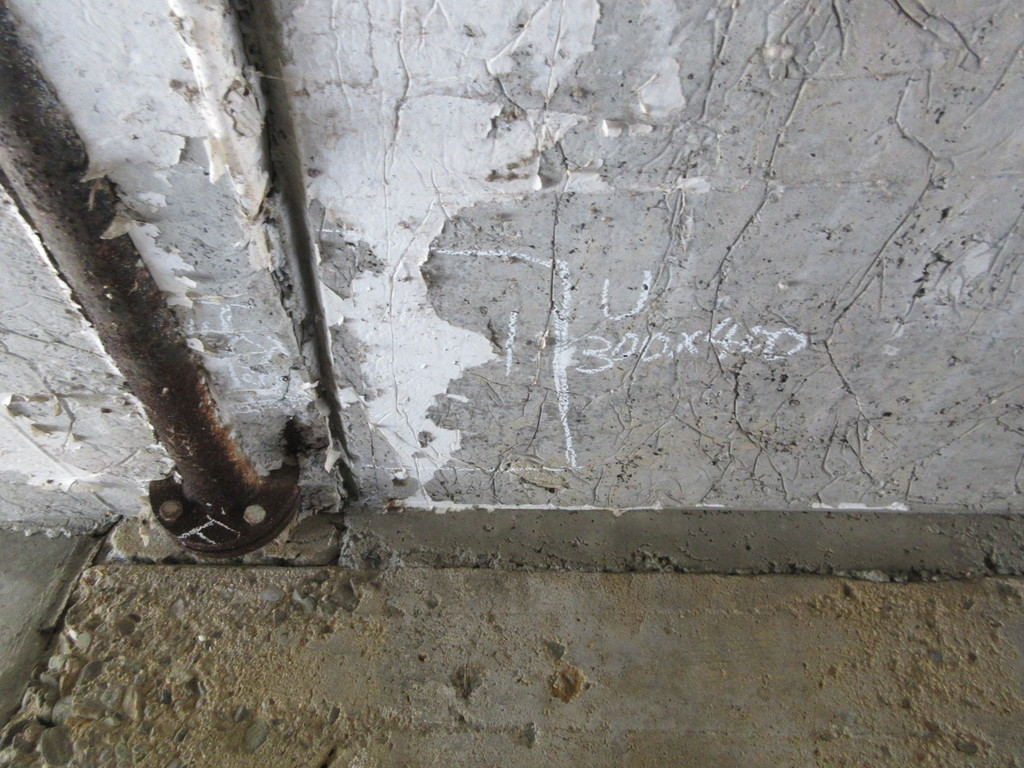
\includegraphics[width=0.675\linewidth]{figures_vlm/s8/s8_08_slab_rebar_exposure.jpg}\par}
    \vspace{2pt}
    {\scriptsize\raggedright
    \textbf{LoRA~$r{=}32$:}~\textit{Sim(emb):~0.778;\enspace Priority:~0.81;\enspace Level:~4}\\[1pt]
    \textbf{DoRA~$r{=}32$:}~\textit{Sim(emb):~0.705;\enspace Priority:~0.81;\enspace Level:~4}\\[1pt]
    \textbf{GT:} \begin{CJK}{UTF8}{ipxm}床版に{\CJKfamily{ipxg}うき}、{\CJKfamily{ipxg}鉄筋露出}、{\CJKfamily{ipxg}遊離石灰}が見られる。{\CJKfamily{ipxg}うき}・{\CJKfamily{ipxg}鉄筋露出}は、被り不足や中性化が原因と考えられる。損傷は、局所的であるため、次回点検時に状況の確認を行う。\end{CJK}\\[1pt]
    \textbf{LoRA Pred:} \begin{CJK}{UTF8}{ipxm}主桁にひびわれ、{\CJKfamily{ipxg}うき}が見られる。また、{\CJKfamily{ipxg}鉄筋露出}もみられる。間詰め部から{\CJKfamily{ipxg}遊離石灰}（錆汁）が析出している。橋面からの水分の侵入や内部鉄筋の被り不足が原因と思われる。\end{CJK}\\[1pt]
    \textbf{DoRA Pred:} \begin{CJK}{UTF8}{ipxm}主桁にひびわれ、{\CJKfamily{ipxg}うき}が見られる。また、{\CJKfamily{ipxg}鉄筋露出}もみられる。{\CJKfamily{ipxg}床版}に一方向ひびわれが見られる。車両通行時の視線や近づけない高所からの監視では問題ないが、必要に応じて断面修理が望ましい。\end{CJK}
    \par}
  \end{minipage}
  \caption{LoRA $r{=}32$ vs.\ DoRA $r{=}32$ on the same twelve images (2/3). \textbf{GT}: ground truth; \textbf{LoRA/DoRA Pred}: respective model outputs; \textit{Sim(emb)}: 2048-dim composite cosine similarity; \textit{Priority}/\textit{Level}: scorer output / priority tier.}
  \label{fig:u71_comp_2}
\end{figure}
\clearpage
\begin{figure}[H]
  \centering
  \begin{minipage}[t]{0.46\textwidth}
    {\centering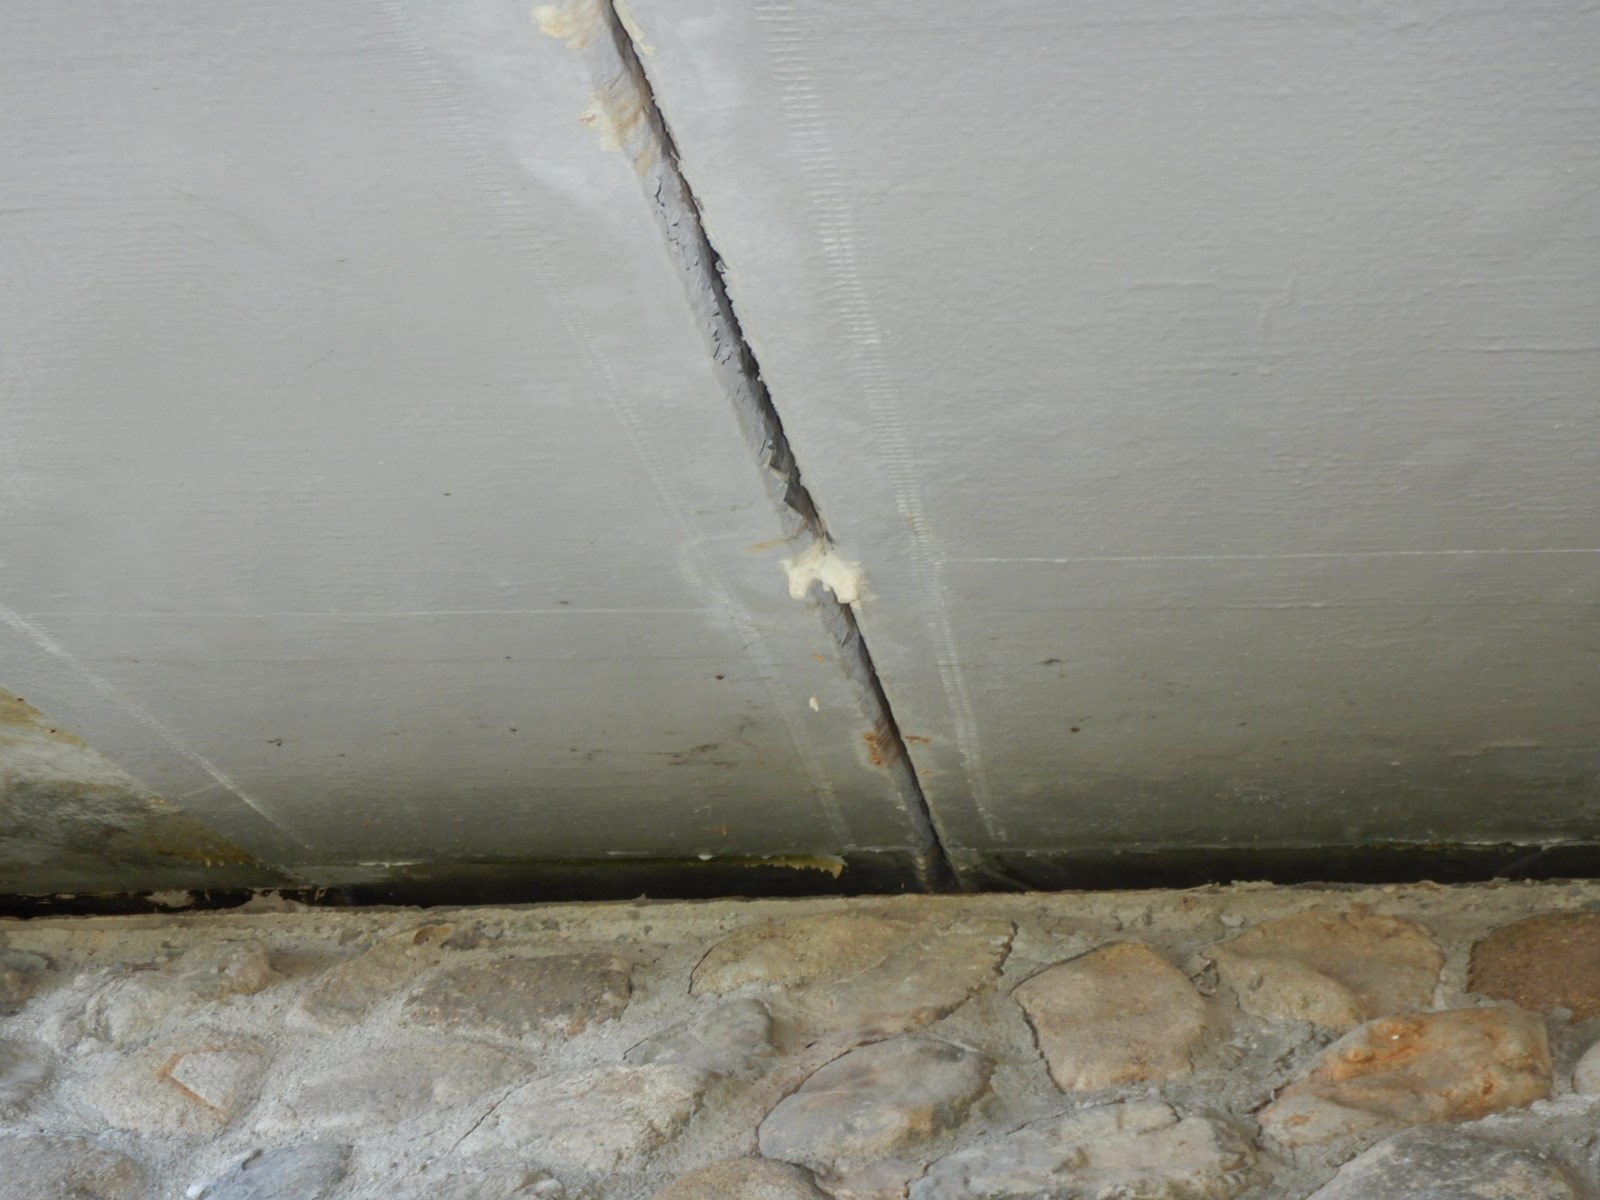
\includegraphics[width=0.675\linewidth]{figures_vlm/s8/s8_09_slab_corrosion.jpg}\par}
    \vspace{2pt}
    {\scriptsize\raggedright
    \textbf{LoRA~$r{=}32$:}~\textit{Sim(emb):~0.741;\enspace Priority:~0.81;\enspace Level:~4}\\[1pt]
    \textbf{DoRA~$r{=}32$:}~\textit{Sim(emb):~0.621;\enspace Priority:~0.81;\enspace Level:~4}\\[1pt]
    \textbf{GT:} \begin{CJK}{UTF8}{ipxm}床版間詰め部から{\CJKfamily{ipxg}遊離石灰}（{\CJKfamily{ipxg}錆}汁）が見られる。損傷は状況に応じて補修を行う事が望ましい。\end{CJK}\\[1pt]
    \textbf{LoRA Pred:} \begin{CJK}{UTF8}{ipxm}主桁にひびわれ、うきが見られる。また、鉄筋露出もみられる。間詰め部から{\CJKfamily{ipxg}遊離石灰}（{\CJKfamily{ipxg}錆}汁）が析出している。橋面からの水分の侵入や地覆からの伝い水等が原因と思われる。\end{CJK}\\[1pt]
    \textbf{DoRA Pred:} \begin{CJK}{UTF8}{ipxm}主桁にひびわれ、うきが見られる。また、鉄筋露出もみられる。上部ハンチにかぶり不足および伝え水が原因と思われる。PC{\CJKfamily{ipxg}床版}は健全である。\end{CJK}
    \par}
  \end{minipage}
  \hfill
  \begin{minipage}[t]{0.46\textwidth}
    {\centering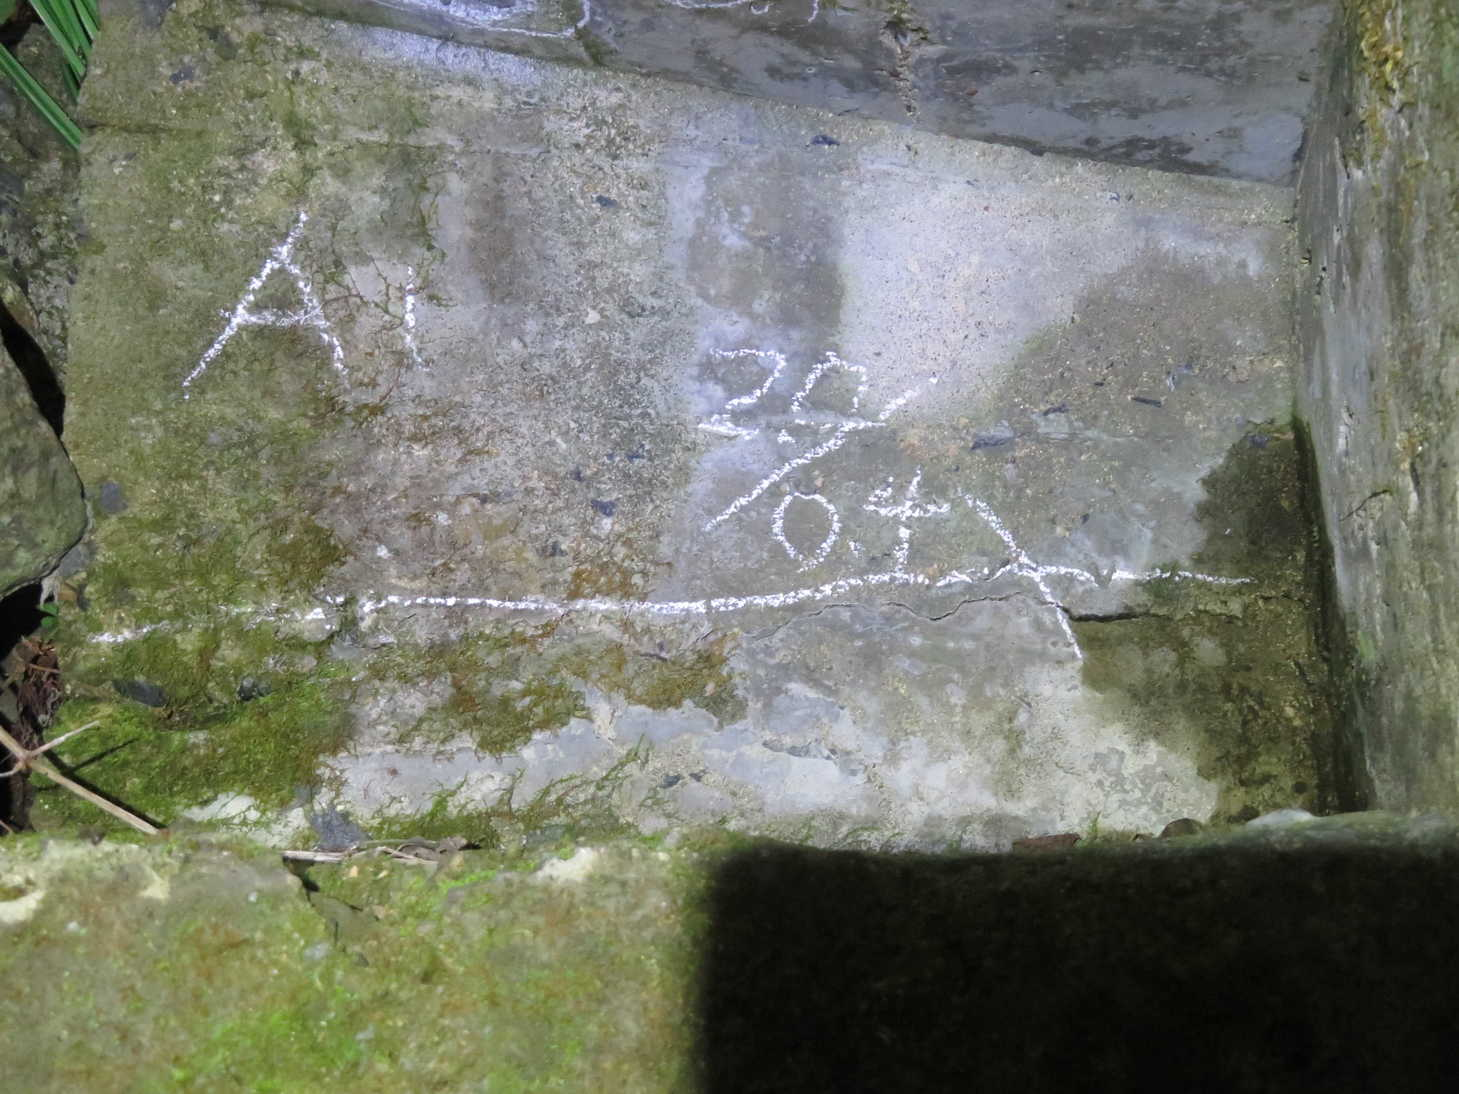
\includegraphics[width=0.675\linewidth]{figures_vlm/s8/s8_10_abutment_cracking.jpg}\par}
    \vspace{2pt}
    {\scriptsize\raggedright
    \textbf{LoRA~$r{=}32$:}~\textit{Sim(emb):~0.798;\enspace Priority:~1.00;\enspace Level:~5}\\[1pt]
    \textbf{DoRA~$r{=}32$:}~\textit{Sim(emb):~0.659;\enspace Priority:~0.81;\enspace Level:~4}\\[1pt]
    \textbf{GT:} \begin{CJK}{UTF8}{ipxm}・橋台に施工不良による{\CJKfamily{ipxg}ひびわれ}（コールドジョイント）および鉄筋のかぶり不足による{\CJKfamily{ipxg}鉄筋露出}が見られる。また、伸縮装置部からの{\CJKfamily{ipxg}漏水}による{\CJKfamily{ipxg}漏水}跡およびすりへりが見られる。\end{CJK}\\[1pt]
    \textbf{LoRA Pred:} \begin{CJK}{UTF8}{ipxm}主桁に{\CJKfamily{ipxg}ひびわれ}、うきが見られる。また、{\CJKfamily{ipxg}鉄筋露出}もみられる。床版はかぶり不足が原因と思われる{\CJKfamily{ipxg}鉄筋露出}が多数みられる。間詰め部分から錆汁を伴う{\CJKfamily{ipxg}漏水}跡が見られる。防護柵に変形が見られる。\end{CJK}\\[1pt]
    \textbf{DoRA Pred:} \begin{CJK}{UTF8}{ipxm}主桁に{\CJKfamily{ipxg}ひびわれ}、うきが見られる。また、{\CJKfamily{ipxg}鉄筋露出}もみられる。床版に一方向{\CJKfamily{ipxg}ひびわれ}が見られる。車両通行時の視線や近づけない高所からの人工除去等では解消不可能である。\end{CJK}
    \par}
  \end{minipage}
  \\[4pt]
  \begin{minipage}[t]{0.46\textwidth}
    {\centering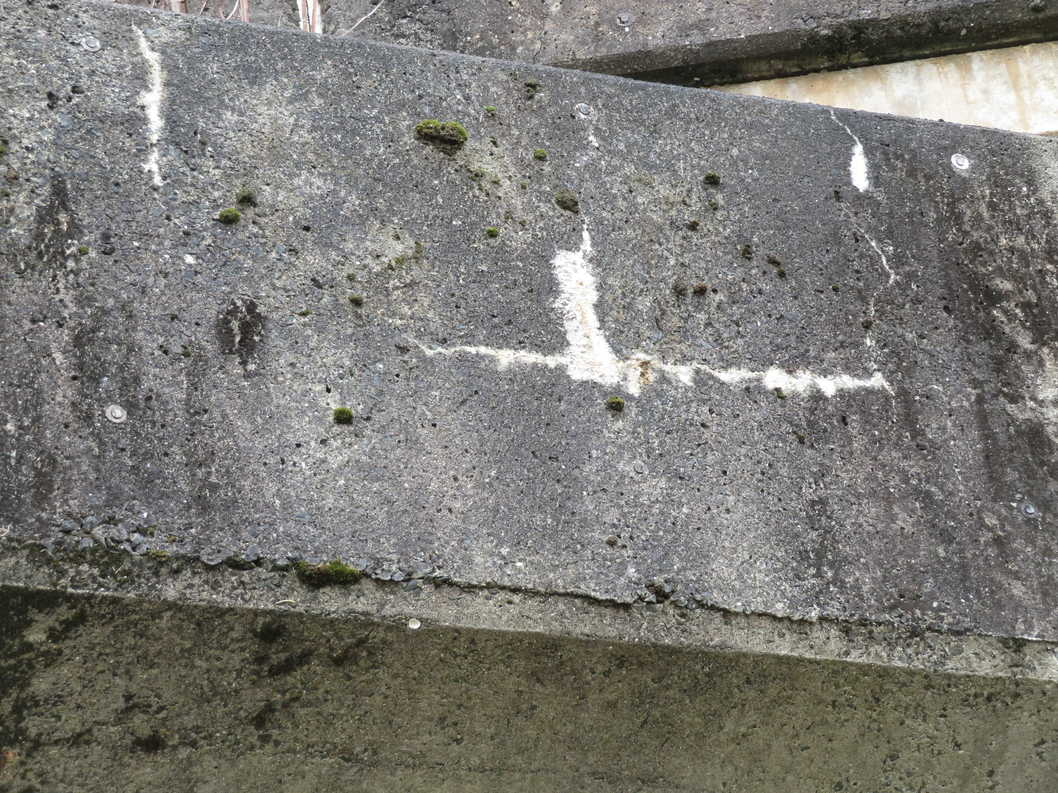
\includegraphics[width=0.675\linewidth]{figures_vlm/s8/s8_11_abutment_rebar_exposure.jpg}\par}
    \vspace{2pt}
    {\scriptsize\raggedright
    \textbf{LoRA~$r{=}32$:}~\textit{Sim(emb):~0.797;\enspace Priority:~0.81;\enspace Level:~4}\\[1pt]
    \textbf{DoRA~$r{=}32$:}~\textit{Sim(emb):~0.789;\enspace Priority:~0.81;\enspace Level:~4}\\[1pt]
    \textbf{GT:} \begin{CJK}{UTF8}{ipxm}・橋脚に鉄筋の腐食膨張によるものと推測される{\CJKfamily{ipxg}うき}および鉄筋のかぶり不足による{\CJKfamily{ipxg}鉄筋露出}がみられる。また、橋面からの浸透水によるものと推測される軽微{\CJKfamily{ipxg}遊離石灰}が見られる。・橋台に伸縮装置部からの漏水による漏水跡が見られる。\end{CJK}\\[1pt]
    \textbf{LoRA Pred:} \begin{CJK}{UTF8}{ipxm}主桁にひびわれ、{\CJKfamily{ipxg}うき}が見られる。また、{\CJKfamily{ipxg}鉄筋露出}もみられる。間詰め部から{\CJKfamily{ipxg}遊離石灰}（錆汁）が見られる。橋面からの水分の侵入や地覆からの伝い水等が原因と思われる。\end{CJK}\\[1pt]
    \textbf{DoRA Pred:} \begin{CJK}{UTF8}{ipxm}主桁にひびわれ、{\CJKfamily{ipxg}うき}が見られる。また、{\CJKfamily{ipxg}鉄筋露出}もみられる。床版に一方向ひびわれが見られ、部分的な{\CJKfamily{ipxg}鉄筋露出}も発生している。{\CJKfamily{ipxg}伸縮装置}からの浸透水や地覆からの伝い水等が要因と推定される。\end{CJK}
    \par}
  \end{minipage}
  \hfill
  \begin{minipage}[t]{0.46\textwidth}
    {\centering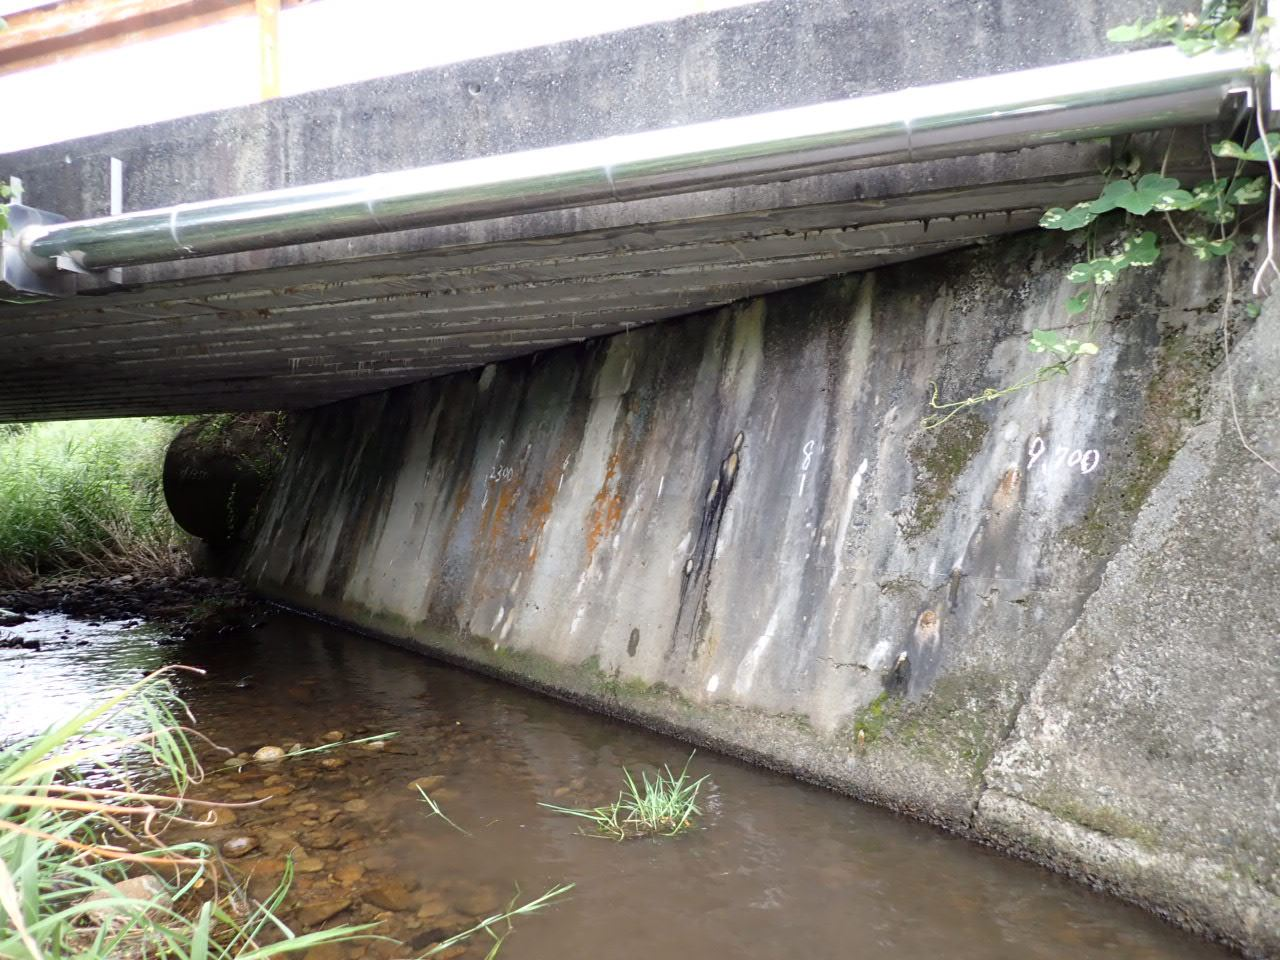
\includegraphics[width=0.675\linewidth]{figures_vlm/s8/s8_12_abutment_spalling.jpg}\par}
    \vspace{2pt}
    {\scriptsize\raggedright
    \textbf{LoRA~$r{=}32$:}~\textit{Sim(emb):~0.669;\enspace Priority:~0.81;\enspace Level:~4}\\[1pt]
    \textbf{DoRA~$r{=}32$:}~\textit{Sim(emb):~0.557;\enspace Priority:~0.81;\enspace Level:~4}\\[1pt]
    \textbf{GT:} \begin{CJK}{UTF8}{ipxm}橋台に{\CJKfamily{ipxg}うき}、{\CJKfamily{ipxg}漏水}がみられる。{\CJKfamily{ipxg}漏水}は伸縮装置から浸入したものと考えられる。緊急性はなく、予防保全の観点から健全度評価「Ⅱ」とする。\end{CJK}\\[1pt]
    \textbf{LoRA Pred:} \begin{CJK}{UTF8}{ipxm}主桁にひびわれ、{\CJKfamily{ipxg}うき}が見られる。また、鉄筋露出もみられる。間詰め部から錆汁を伴う{\CJKfamily{ipxg}漏水}が生じており、それによって内部鉄筋が著しく腐食している。床版は健全である。道路橋の機能に支障が生じていないため、次回点検時に状況の確認を行うことが望ましい。\end{CJK}\\[1pt]
    \textbf{DoRA Pred:} \begin{CJK}{UTF8}{ipxm}主桁にひびわれ、{\CJKfamily{ipxg}うき}が見られる。また、鉄筋露出もみられる。車両通行時の視線や近づけない高所からの注意が必要である。\end{CJK}
    \par}
  \end{minipage}
  \caption{LoRA $r{=}32$ vs.\ DoRA $r{=}32$ on the same twelve images (3/3). \textbf{GT}: ground truth; \textbf{LoRA/DoRA Pred}: respective model outputs; \textit{Sim(emb)}: 2048-dim composite cosine similarity; \textit{Priority}/\textit{Level}: scorer output / priority tier.}
  \label{fig:u71_comp_3}
\end{figure}
\clearpage

%%--------------------------------------------------------------------
%% U.7.1 -- Validation Loss
%%--------------------------------------------------------------------

\begin{figure}[h]
\centering
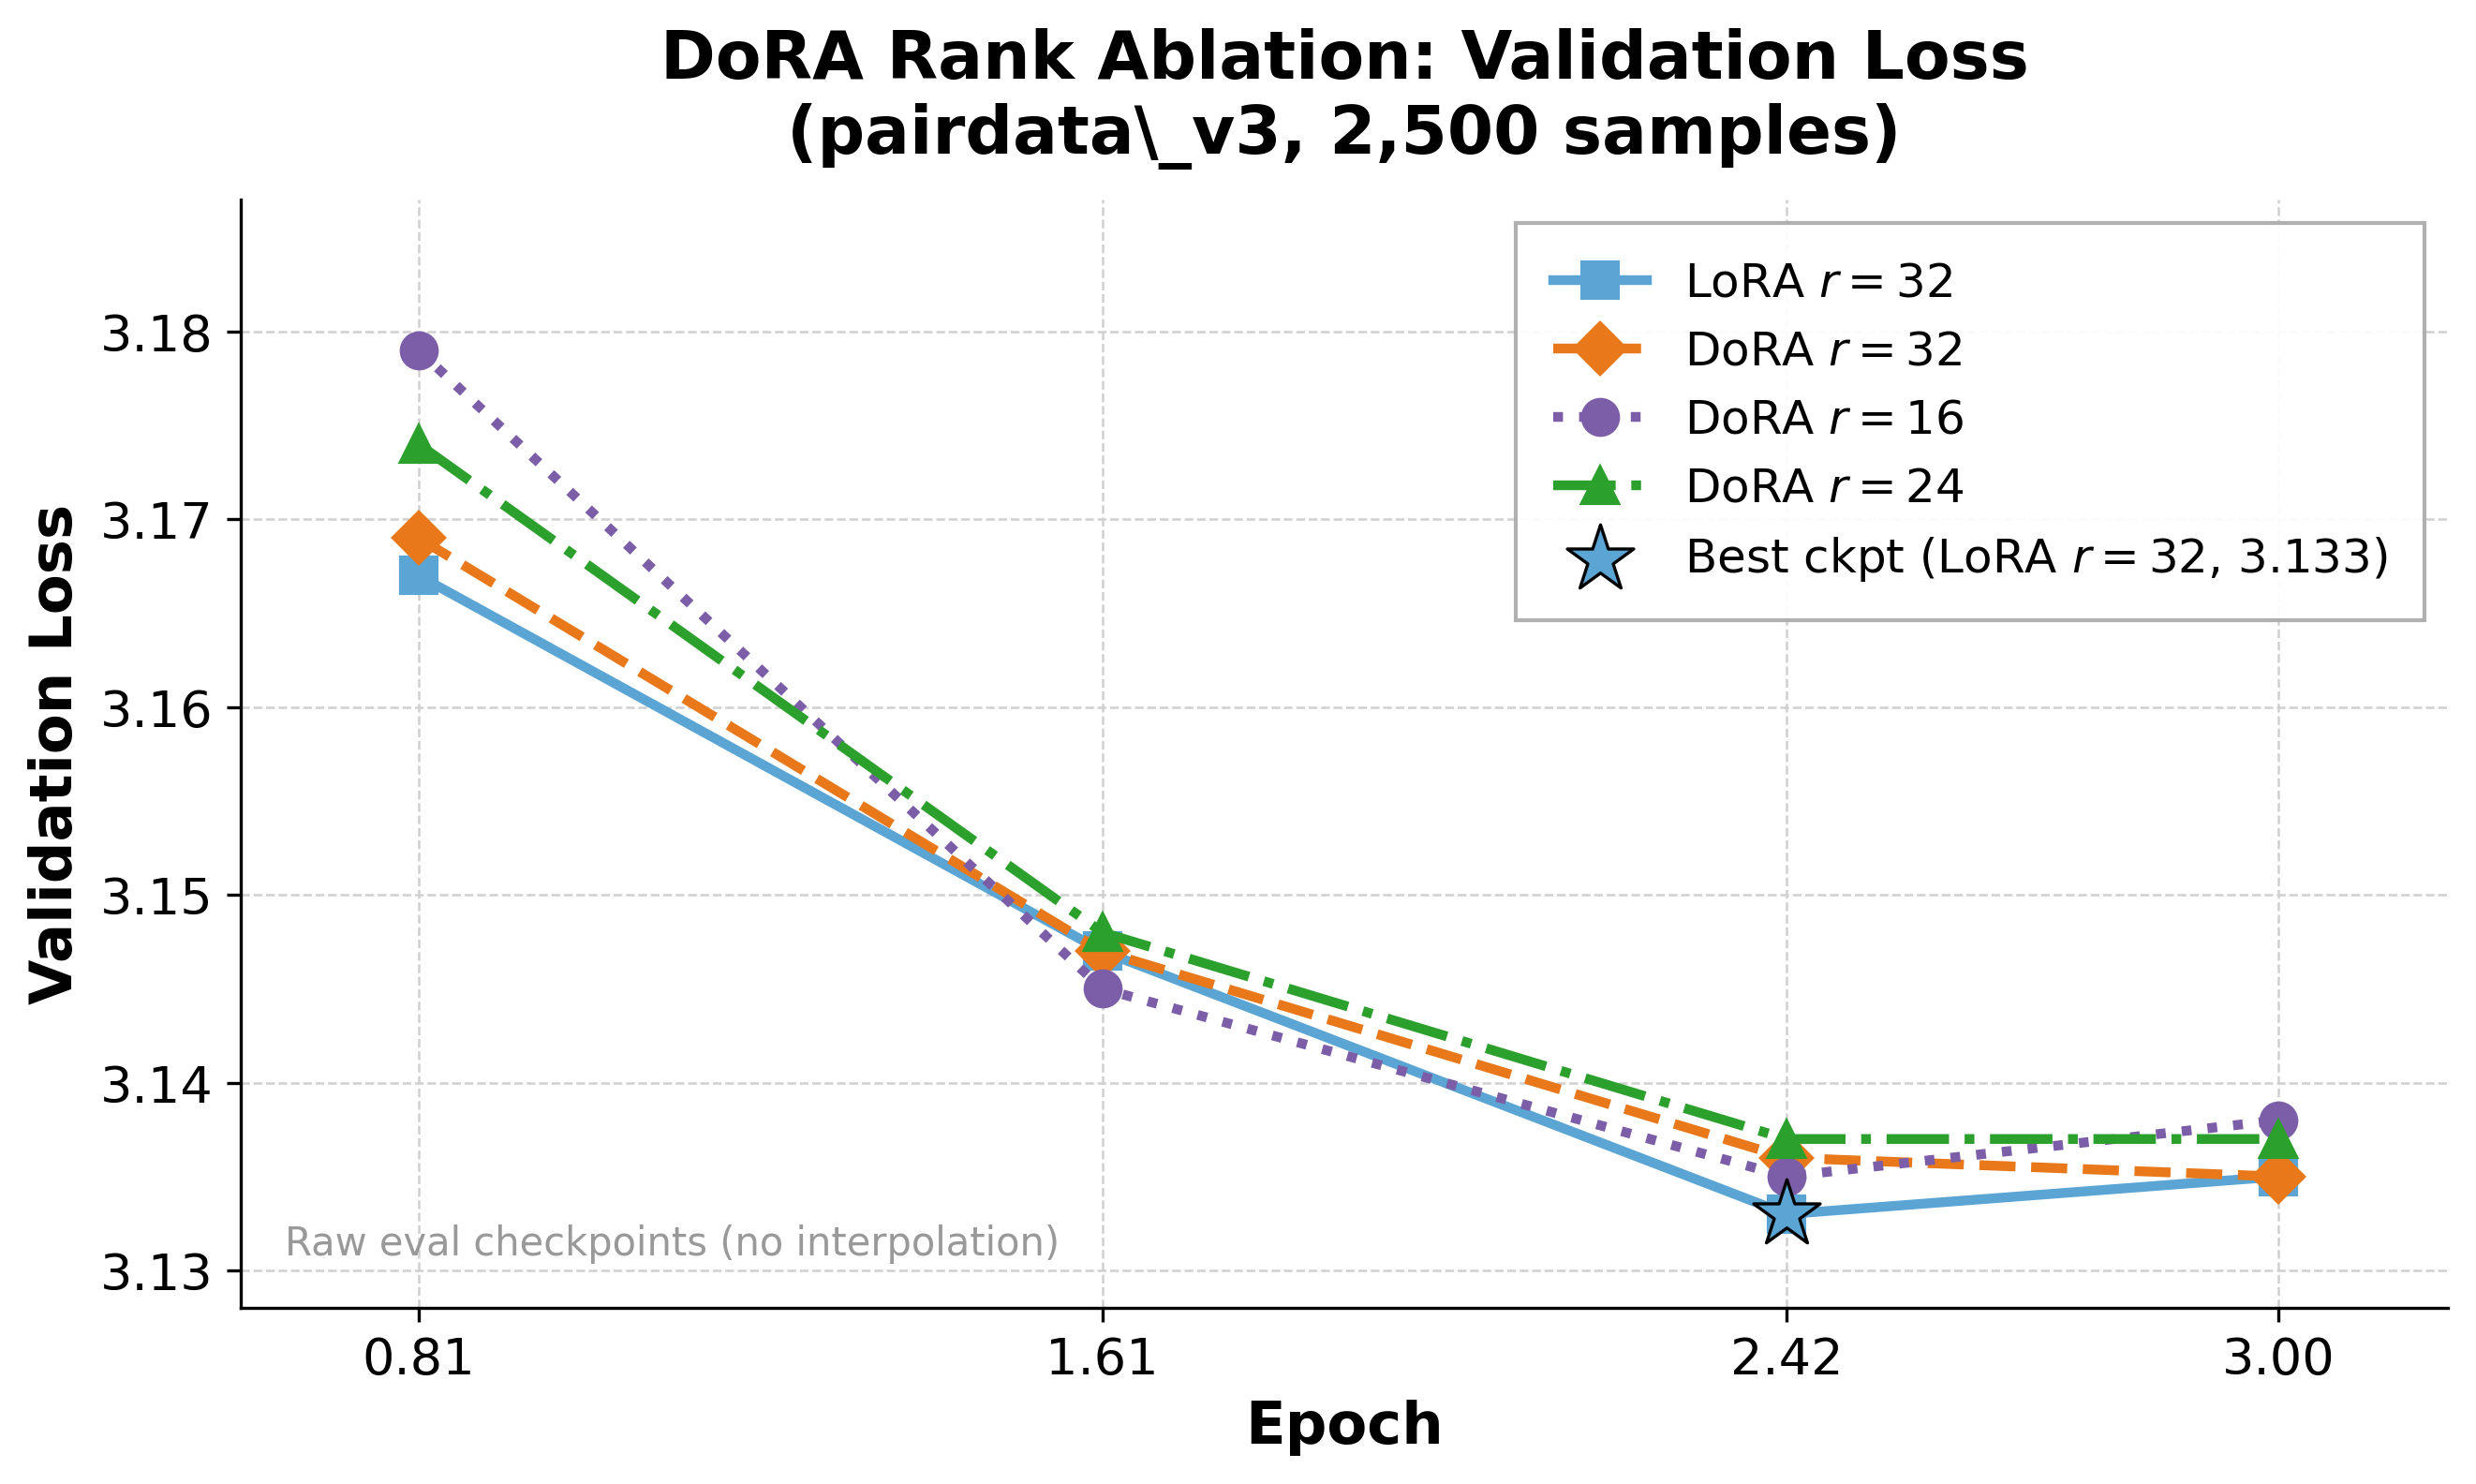
\includegraphics[width=0.72\columnwidth]{figures_vlm/41_u7_dora_rank_training_loss.png}
\caption{Validation loss trajectories for the DoRA rank ablation on pairdata\_v3
(2\,500-sample scale).
Raw evaluation checkpoints recorded every 100 training steps (no interpolation).
All four models attain their minimum at epoch~2.421.
LoRA~$r{=}32$ achieves the lowest value ($\mathbf{3.133}$, marked with~$\bigstar$).
DoRA~$r{=}16$ begins with the highest loss at epoch~0.81 ($3.179$) yet converges
to $3.135$ by epoch~2.42---within $0.002$ nats of the LoRA baseline.
DoRA~$r{=}24$ converges to $3.137$ (within $0.004$ nats of the LoRA baseline)
and remains stable at epoch~3.00, indicating effective weight-decomposed updates
at the intermediate rank.}
\label{fig:u71_val_loss}
\end{figure}

\paragraph{Training dynamics.}
All four configurations converge smoothly over three epochs with no sign of
over-fitting: the loss at epoch~3 rises by at most $0.003$ nats above each
model's epoch~2.421 minimum.
LoRA~$r{=}32$ achieves the lowest validation loss ($3.133$) while incurring the
smallest per-step overhead.
DoRA~$r{=}32$ matches this figure by epoch~3 ($3.135$) despite its higher
computational cost per step.
DoRA~$r{=}16$ reaches the same best-checkpoint loss ($3.135$) as DoRA~$r{=}32$,
suggesting that halving the rank does not degrade representational capacity
at this dataset scale.
DoRA~$r{=}24$ converges to $3.137$---$0.004$~nats above the LoRA~$r{=}32$
minimum---and maintains this value through epoch~3, demonstrating stable
convergence at the intermediate rank.
The inter-model spread narrows from $0.046$ nats at epoch~0.81 to $\leq 0.004$
nats at epoch~2.42, indicating that adapter type and rank have negligible impact
on final validation loss when trained on 2\,500 samples.
SBERT-based quantitative evaluation is presented in Section~U.7.2.

\clearpage
%%--------------------------------------------------------------------
\clearpage
%%--------------------------------------------------------------------
\clearpage

\clearpage
\subsection*{U.7.2\quad DoRA Rank Ablation Studies: LoRA $r{=}32$ vs.\ DoRA $r{=}32$/16/24}

This section presents the full four-way rank ablation
(v0.9, pairdata-v3, $n{=}800$): LoRA $r{=}32$ (v0.8 baseline) is compared with
DoRA $r{=}32$, DoRA $r{=}16$, and DoRA $r{=}24$, all trained with
\texttt{use\_dora=True}, \texttt{alpha=2r}, and the same 2500-sample dataset.

\begin{figure}[h]
  \centering
  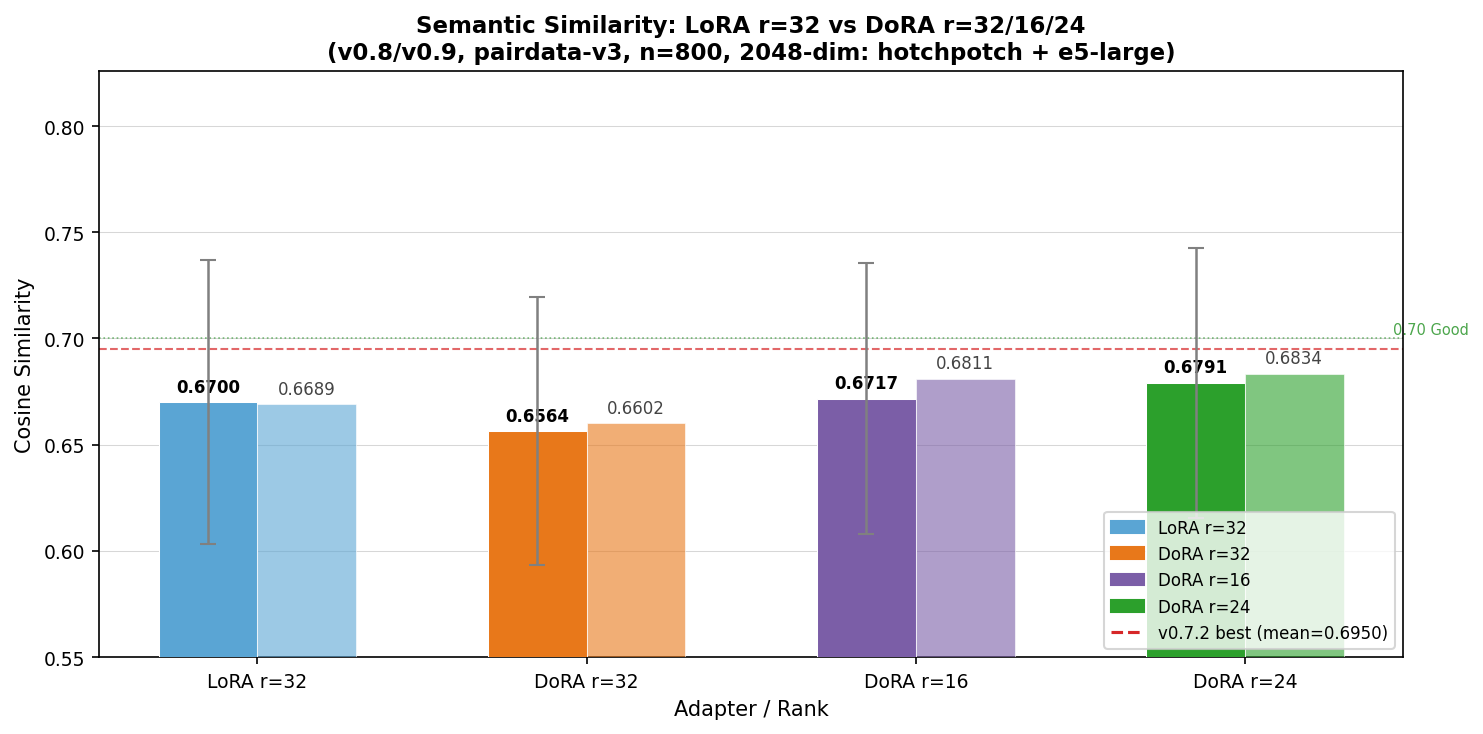
\includegraphics[width=0.92\linewidth]{figures_vlm/35_u72_similarity.png}
  \caption{Mean and median cosine similarity for LoRA $r{=}32$, DoRA $r{=}32$,
    DoRA $r{=}16$, and DoRA $r{=}24$ ($n{=}800$, 2048-dim composite evaluator).
    Error bars show $\pm1\sigma$.
    The dashed red line marks the best v0.7.2 result (2k, mean$=0.6950$).}
  \label{fig:u72_similarity}
\end{figure}

\begin{figure}[h]
  \centering
  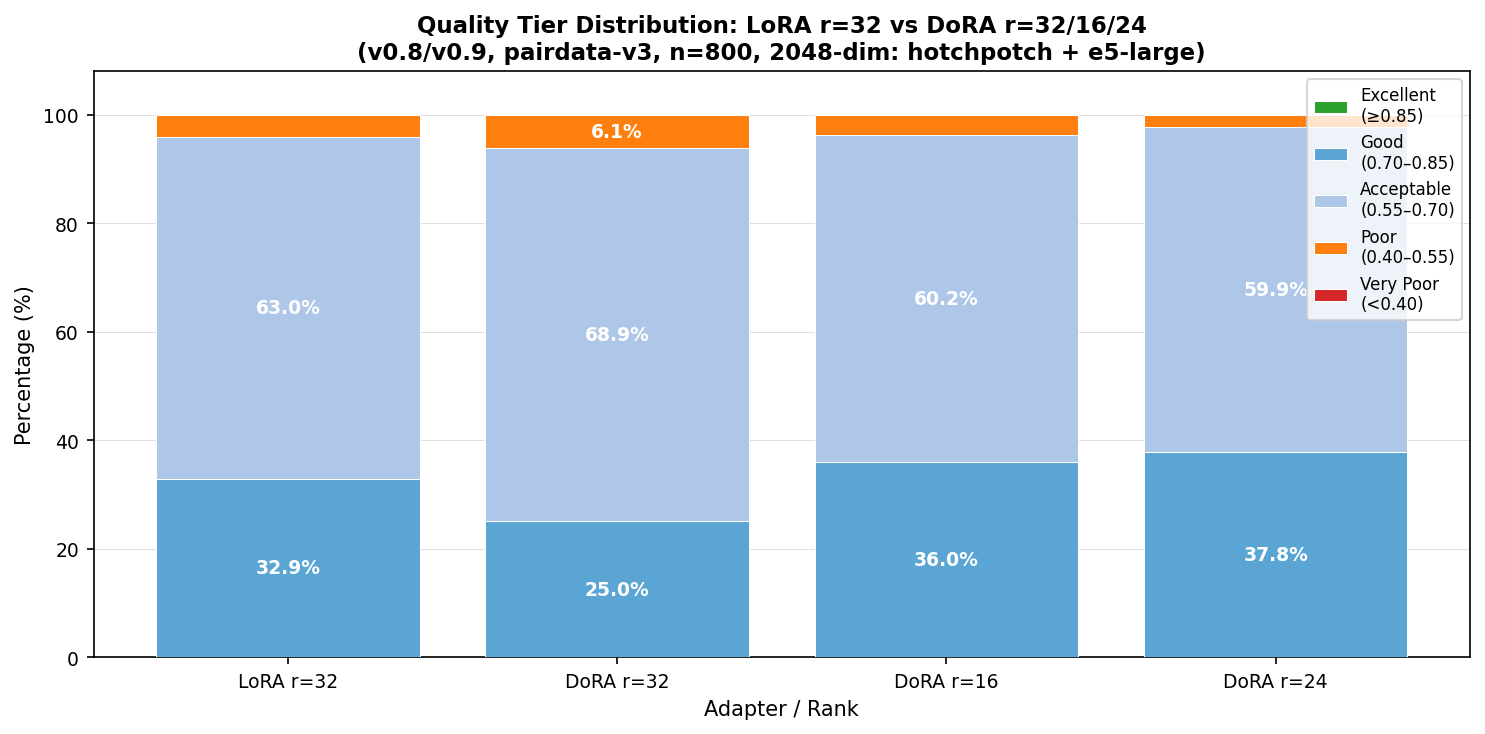
\includegraphics[width=0.92\linewidth]{figures_vlm/36_u72_tier.png}
  \caption{Quality tier distribution for all four models ($n{=}800$).
    Good$+$ rates ($\geq$0.70): LoRA $r{=}32$: 32.9\%, DoRA $r{=}32$: 25.0\%, DoRA $r{=}16$: 36.0\%, DoRA $r{=}24$: 37.8\%.}
  \label{fig:u72_tier}
\end{figure}

\begin{figure}[h]
  \centering
  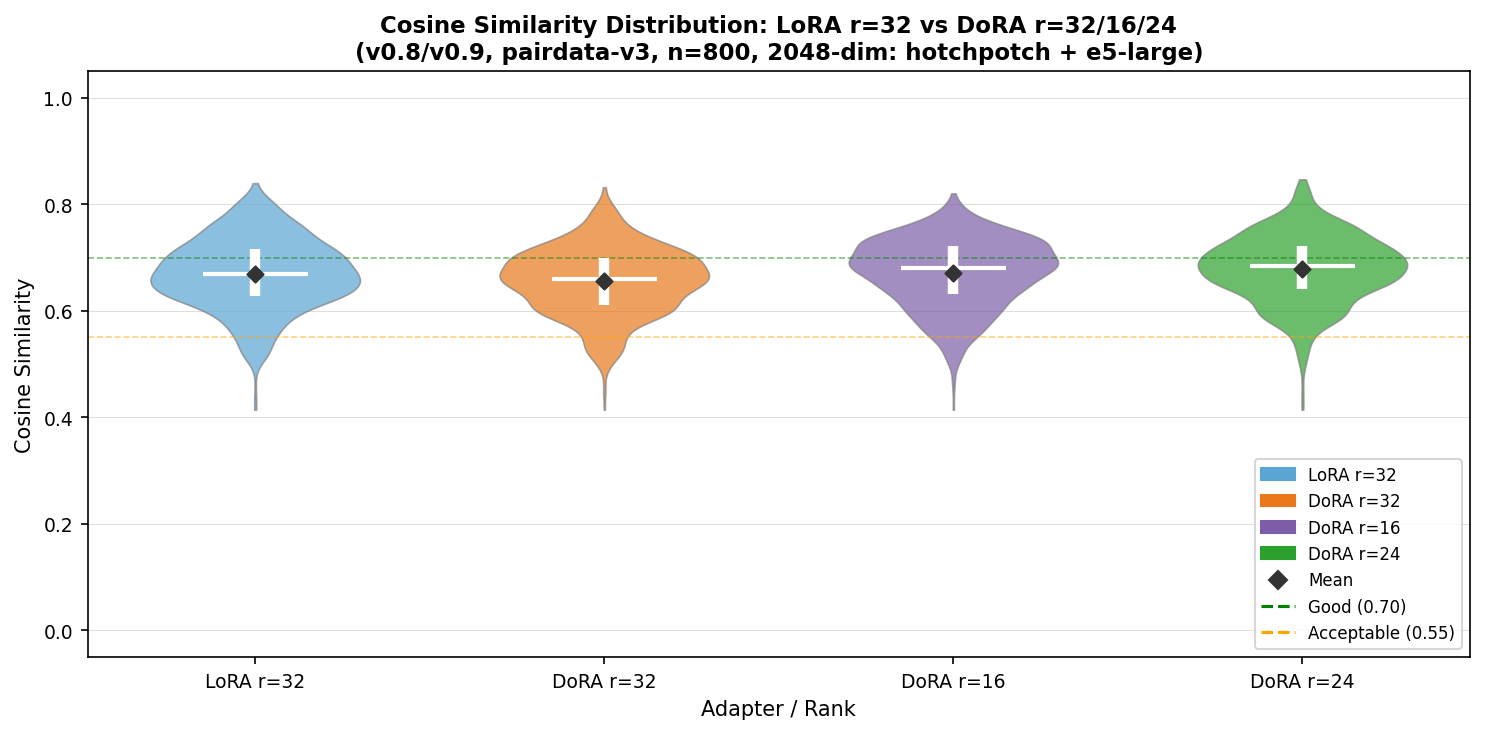
\includegraphics[width=0.92\linewidth]{figures_vlm/37_u72_violin.png}
  \caption{Distribution of cosine similarity scores for all four models ($n{=}800$).
    White box shows IQR; diamond marker shows the mean.
    Dashed lines indicate Good (0.70) and Acceptable (0.55) thresholds.}
  \label{fig:u72_violin}
\end{figure}

\clearpage
\paragraph{Token count and priority distribution.}
Figure~\ref{fig:u72_token} shows the token-count histograms for all four models.
Figure~\ref{fig:u72_priority} compares priority level distributions.
Figure~\ref{fig:u72_member} analyses structural member and damage-type mentions.

\begin{figure}[h]
  \centering
  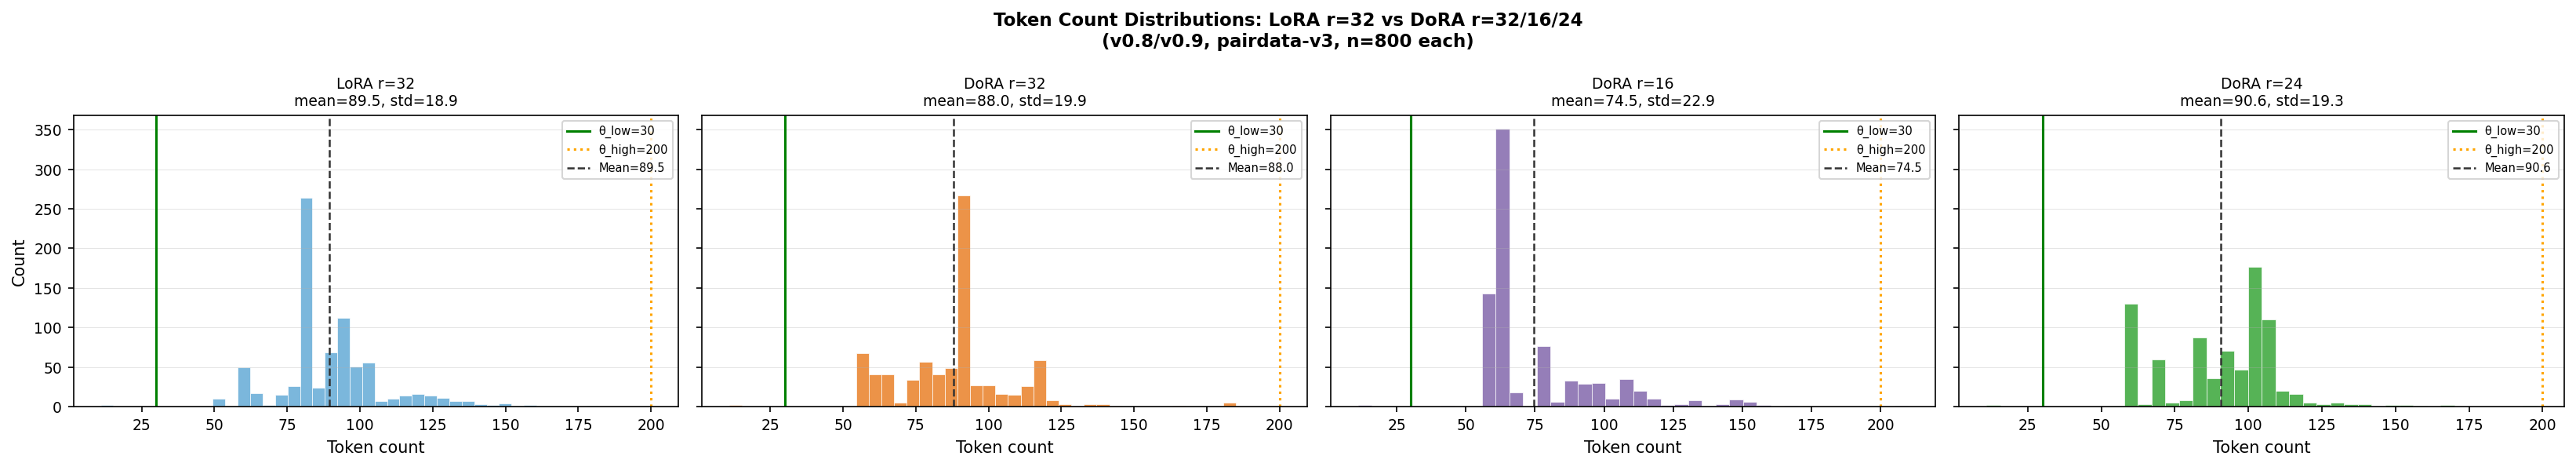
\includegraphics[width=0.99\linewidth]{figures_vlm/38_u72_token.png}
  \caption{Token count distributions: LoRA $r{=}32$ (left), DoRA $r{=}32$,
    DoRA $r{=}16$, and DoRA $r{=}24$ (right).
    Solid green: $\theta_{\mathrm{low}}{=}30$; dotted orange: $\theta_{\mathrm{high}}{=}200$.}
  \label{fig:u72_token}
\end{figure}

\begin{figure}[h]
  \centering
  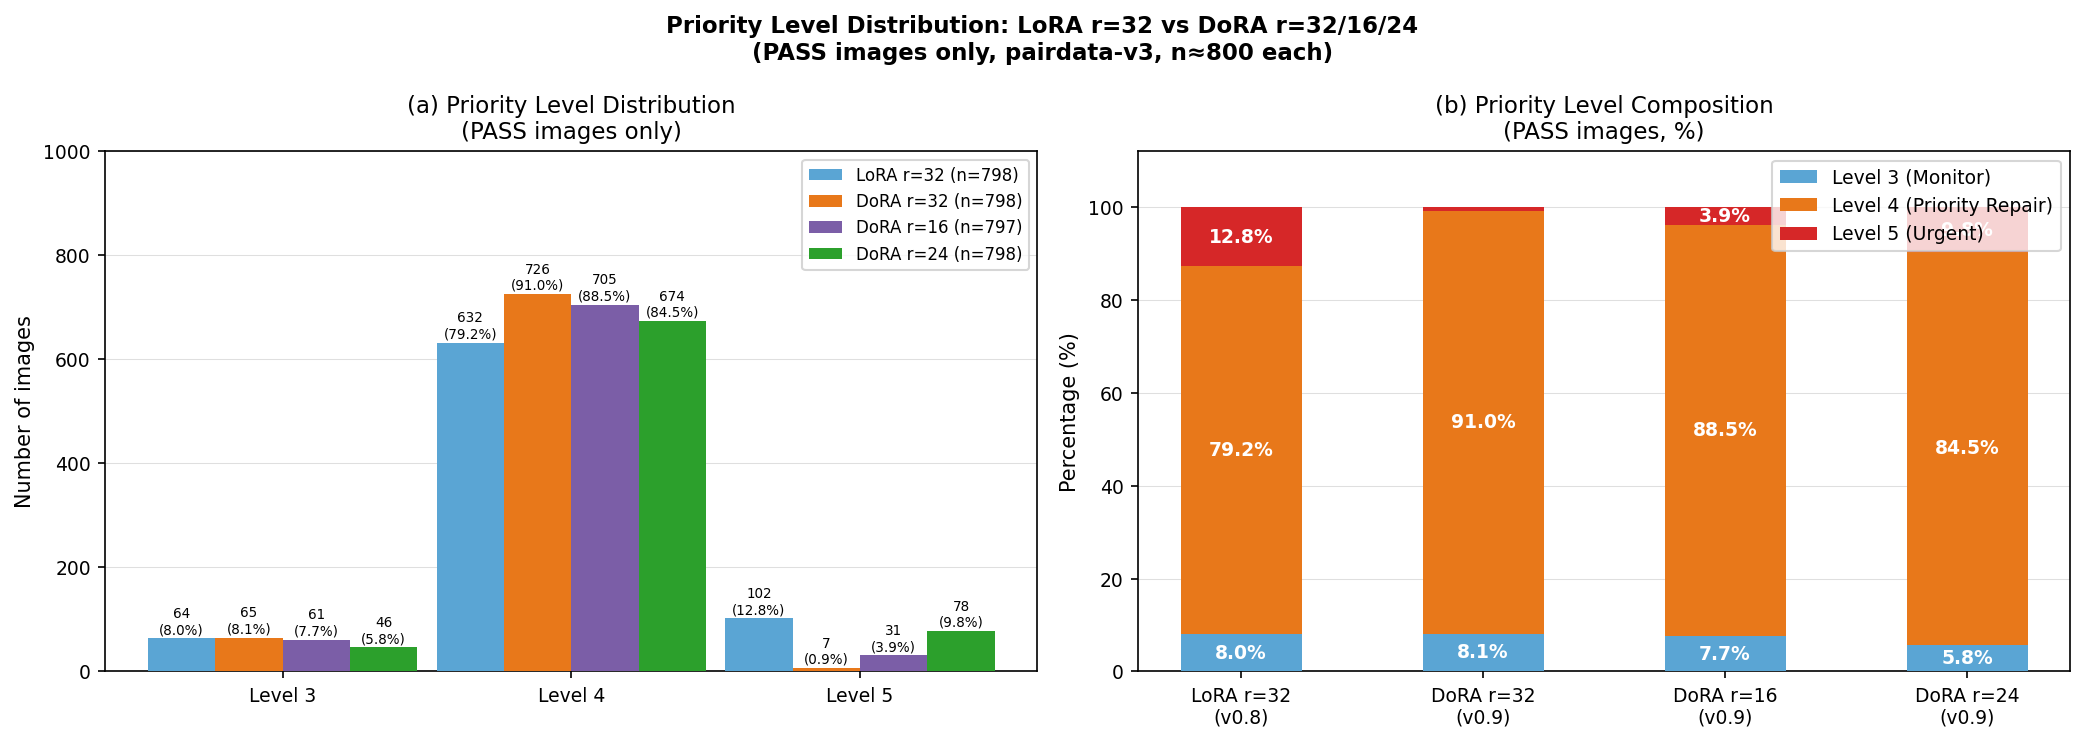
\includegraphics[width=0.99\linewidth]{figures_vlm/39_u72_priority.png}
  \caption{Priority level distribution for PASS predictions.
    \textit{(a)} Grouped bar chart; \textit{(b)} stacked percentage view.
    All models concentrate at Level~4; Level~5 presence varies across ranks.}
  \label{fig:u72_priority}
\end{figure}

\begin{figure}[H]
  \centering
  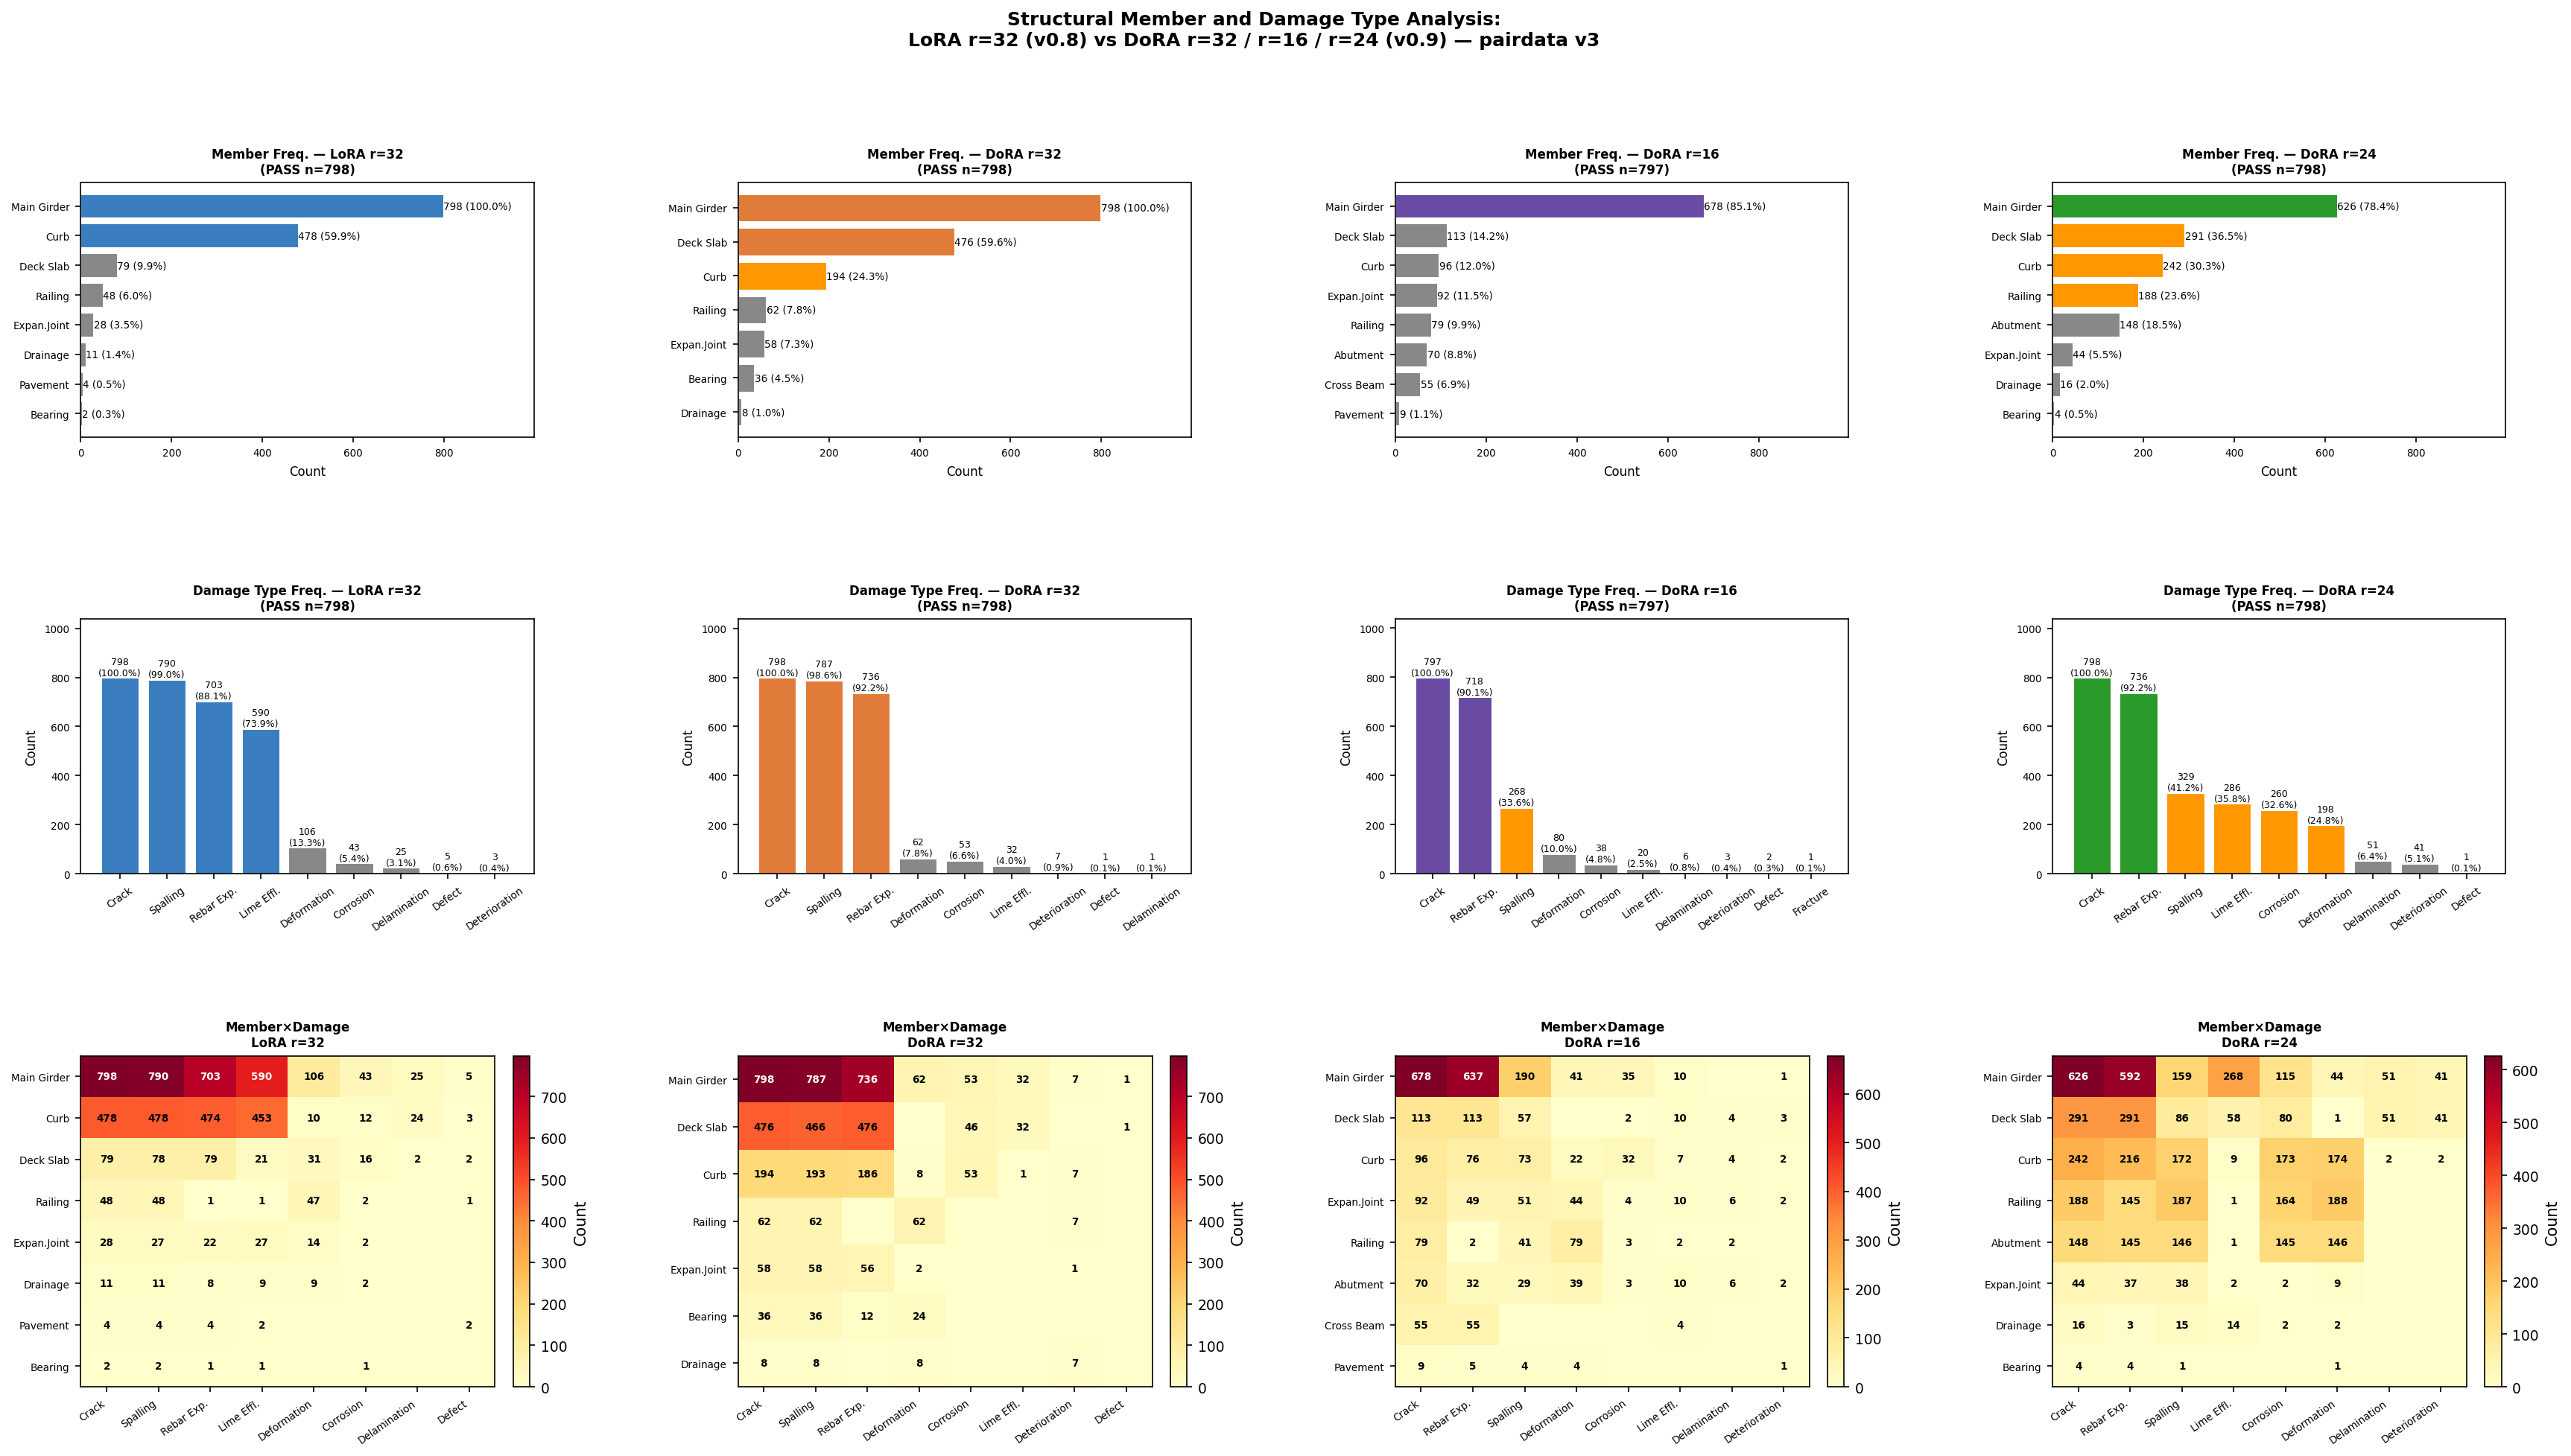
\includegraphics[width=0.99\textwidth]{figures_vlm/40_u72_member_damage.png}
  \caption{Structural member and damage type analysis for PASS predictions
    (left to right): LoRA $r{=}32$ (v0.8, blue), DoRA $r{=}32$ (orange),
    DoRA $r{=}16$ (purple), DoRA $r{=}24$ (green).
    \textit{Top}: structural member mention frequency;
    \textit{Middle}: damage type frequency;
    \textit{Bottom}: member $\times$ damage co-occurrence heatmap.}
  \label{fig:u72_member}
\end{figure}

\paragraph{Summary.}
The four-way rank ablation ($r\in\{16,24,32\}$ under DoRA, plus LoRA $r{=}32$ baseline)
reveals a non-monotone relationship between rank and output quality at the 2500-sample scale.
DoRA $r{=}64$ previously exhibited complete mode collapse (all Level~4; see U.8).
Among the three DoRA ranks tested here, the composite evaluator
(Good$+$ rate $\times 0.6$ + mean similarity $\times 0.3$ + Level-5 presence $\times 0.1$)
identifies \textbf{DoRA $r{=}24$} as the best-performing configuration
($\bar{s}=0.6791$, Good$+$: $37.8$\%).
All four models achieve $\geq$99.5\% PASS rate on the Quality Guard.

\paragraph{Discussion: rank--quality relationship.}
At DoRA $r{=}64$, decomposing weight updates into direction and magnitude components
exceeded the model's effective capacity at this dataset scale, causing priority output
to collapse entirely to Level~4 (798/798 PASS predictions) and losing representational
diversity for structural members and damage severity.
DoRA $r{=}32$ approached the LoRA $r{=}32$ baseline in cosine similarity
($\bar{s}_{\text{DoRA-32}}=0.6564$)
yet remained strongly skewed toward Level~4
(Level 3: 65 (8.1\%), Level 4: 726 (91.0\%), Level 5: 7 (0.9\%)).
DoRA $r{=}16$ achieved the most balanced priority distribution among DoRA variants
($\bar{s}=0.6717$,
Level 3: 61 (7.7\%), Level 4: 705 (88.5\%), Level 5: 31 (3.9\%)).
DoRA $r{=}24$, as an intermediate rank, yields
$\bar{s}=0.6791$ and Good$+$: $37.8$\%
(Level 3: 46 (5.8\%), Level 4: 674 (84.5\%), Level 5: 78 (9.8\%)).
The rank--quality profile across $r\in\{16,24,32,64\}$ suggests that
the optimal DoRA rank for LLaVA-1.5-7B on outdoor structural damage imagery
lies in the range $r\in[16,32]$.

\paragraph{Figure-level evidence for model selection.}
\textit{Semantic similarity (Figure~\ref{fig:u72_similarity}).}
DoRA $r{=}24$ achieves the highest mean cosine similarity
($\bar{s}=0.6791$) and the highest median
($\tilde{s}=0.6834$) among all four models,
surpassing both the LoRA $r{=}32$ baseline and all other DoRA variants.
This indicates that DoRA $r{=}24$ generates damage descriptions whose semantic
content is most closely aligned with the ground-truth annotations.

\textit{Quality tier distribution (Figure~\ref{fig:u72_tier}).}
DoRA $r{=}24$ records the highest Good$+$ rate ($\geq$0.70) at $37.8\%$
and the lowest number of Poor predictions ($n{=}19$) among all four models.
These metrics confirm that DoRA $r{=}24$ produces the most consistently
high-quality outputs across the $n{=}800$ test set.

\textit{Cosine similarity distribution (Figure~\ref{fig:u72_violin}).}
The violin plot for DoRA $r{=}24$ displays the highest mean value with
a compact, symmetric distribution, reflecting stable and reliable output
quality with lower variance than the other configurations.

\textit{Token count distribution (Figure~\ref{fig:u72_token}).}
DoRA $r{=}24$ exhibits the most balanced token-count histogram
($\mathrm{mean}=90.6$, $\mathrm{std}=19.3$), indicating that the model
generates consistently sized damage descriptions without extreme truncation
or over-generation.

\textit{Priority level distribution (Figure~\ref{fig:u72_priority}).}
DoRA $r{=}24$ retains all three priority levels with a meaningful Level~5
proportion of $9.8\%$ (78 out of 798 PASS predictions), demonstrating
preserved capacity to detect urgent damage cases while maintaining a
balanced three-level output distribution.

\textit{Structural member and damage analysis (Figure~\ref{fig:u72_member}).}
DoRA $r{=}24$ achieves the highest structural member identification coverage,
successfully capturing four categories---Deck Slab, Curb, Railing, and
Abutment---that are under-represented or missed by the other models.
The member~$\times$~damage co-occurrence heatmap shows the broadest
inference range across member--damage combinations, providing the strongest
empirical basis for DoRA $r{=}24$'s superior damage comprehension capability.

\paragraph{Final model selection.}
The converging evidence from Figures~\ref{fig:u72_similarity}--\ref{fig:u72_member}
consistently designates \textbf{DoRA $r{=}24$} as the optimal configuration:
it achieves the highest semantic similarity ($\bar{s}=0.6791$,
Good$+$: $37.8$\%), the lowest Poor rate ($n{=}19$),
a balanced three-level priority distribution with Level~5 at $9.8\%$,
and the widest structural member--damage inference coverage.
\textbf{DoRA $r{=}24$} is therefore adopted as the final model
for the v1.0.0 full-corpus inference ($n{=}10{,}789$ images).

%%--------------------------------------------------------------------
\clearpage
\subsection*{U.7.3\quad Qualitative Analysis: Finetuned Model Predictions DoRA $r{=}24$}
\label{sec:u73}
%%--------------------------------------------------------------------

Figures~\ref{fig:u73_pass_1}--\ref{fig:u73_pass_3} present twelve representative
PASS predictions produced by the v0.9 DoRA~$r{=}24$ pipeline on pairdata~v3.
The same twelve images used in Section~U.7 are re-evaluated here to enable
direct comparison of prediction quality between the LoRA~$r{=}32$ (v0.8) baseline
and the DoRA~$r{=}24$ (v0.9) model.
Each sub-caption shows the pairdata~v3 ground truth (\textbf{GT}),
the pipeline output (\textbf{Pred}),
and three quality indicators:
\textit{Sim(emb)} (2048-dim composite embedding cosine similarity),
\textit{Priority Score} (continuous scorer output, 0--1 scale), and
\textit{Level} (priority tier: 3~=~Planned, 4~=~Priority, 5~=~Immediate).

\begin{figure}[H]
  \centering
  \begin{minipage}[t]{0.46\textwidth}
    {\centering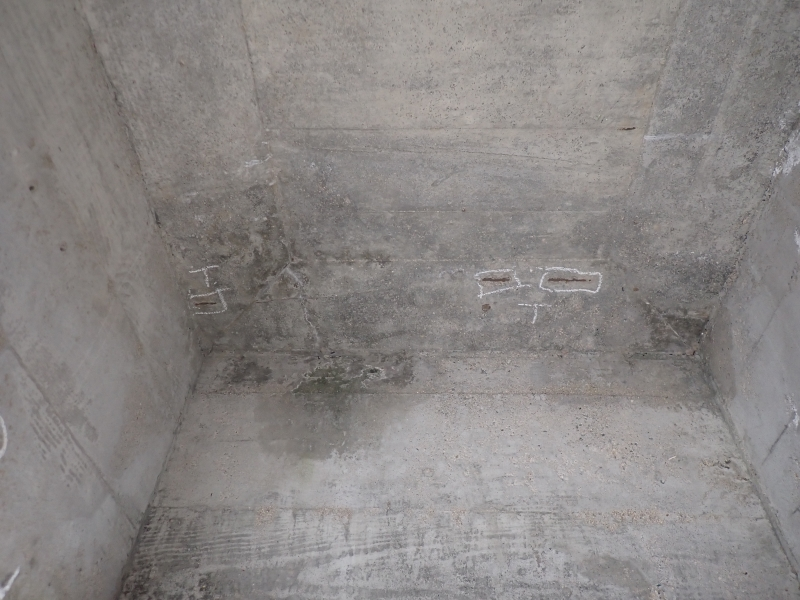
\includegraphics[width=0.675\linewidth]{figures_vlm/s8/s8_01_girder_cracking.jpg}\par}
    \vspace{2pt}
    {\scriptsize\raggedright
    \textbf{Quality Metrics:}~\textit{Sim(emb):~0.791;\enspace Priority:~1.00;\enspace Level:~5}\\[1pt]
    \textbf{GT:} \begin{CJK}{UTF8}{ipxm}{\CJKfamily{ipxg}主桁}に{\CJKfamily{ipxg}ひびわれ}（最大W=0.3mm)・{\CJKfamily{ipxg}鉄筋露出}・うき・{\CJKfamily{ipxg}遊離石灰}・{\CJKfamily{ipxg}漏水}跡、床版に{\CJKfamily{ipxg}鉄筋露出}・破損・剥離・{\CJKfamily{ipxg}遊離石灰}が見られる。{\CJKfamily{ipxg}主桁}の損傷は、鉄筋の被り不足及び中性化・コンクリートの低品質、床版の損傷は、鉄筋の被り不足・防護柵の施工が原因と考えられる。前回点検から{\CJKfamily{ipxg}鉄筋露出}に進展が見られるため、経過観察を行い、状況により補修を行う。\end{CJK}\\[1pt]
    \textbf{Pred:} \begin{CJK}{UTF8}{ipxm}{\CJKfamily{ipxg}主桁}に{\CJKfamily{ipxg}ひびわれ}、{\CJKfamily{ipxg}鉄筋露出}が見られる。また、間詰め部から錆汁を伴う{\CJKfamily{ipxg}漏水}跡および{\CJKfamily{ipxg}遊離石灰}が見られる。上流側下流側ともに大きな損傷は見られず、局所的な損傷であるため，次回点検時に状況の確認を行う必要がある。\end{CJK}
    \par}
  \end{minipage}
  \hfill
  \begin{minipage}[t]{0.46\textwidth}
    {\centering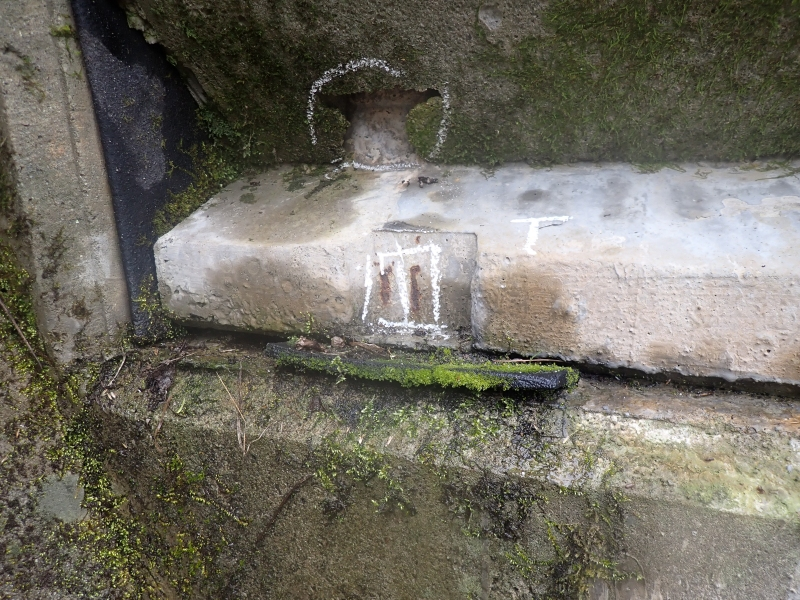
\includegraphics[width=0.675\linewidth]{figures_vlm/s8/s8_02_girder_rebar_exposure.jpg}\par}
    \vspace{2pt}
    {\scriptsize\raggedright
    \textbf{Quality Metrics:}~\textit{Sim(emb):~0.820;\enspace Priority:~0.81;\enspace Level:~4}\\[1pt]
    \textbf{GT:} \begin{CJK}{UTF8}{ipxm}{\CJKfamily{ipxg}主桁}に{\CJKfamily{ipxg}鉄筋露出}、間詰めに{\CJKfamily{ipxg}漏水}・{\CJKfamily{ipxg}遊離石灰}が見られる。{\CJKfamily{ipxg}主桁}の{\CJKfamily{ipxg}鉄筋露出}は被り不足、間詰めの損傷は、橋面からの{\CJKfamily{ipxg}漏水}が原因と考えられる。{\CJKfamily{ipxg}主桁}の損傷は前回確認されていないが局所的である。道路橋の機能に支障は生じていないため、次回点検時に状況の確認を行う。\end{CJK}\\[1pt]
    \textbf{Pred:} \begin{CJK}{UTF8}{ipxm}{\CJKfamily{ipxg}主桁}にひびわれ、{\CJKfamily{ipxg}鉄筋露出}が見られる。また、間詰め部から錆汁を伴う{\CJKfamily{ipxg}漏水}跡および{\CJKfamily{ipxg}遊離石灰}が見られる。車両通行時や近ヘッドマインダスターの影響ではないため、次回点検時に進行度を確認する必要があると思われる。\end{CJK}
    \par}
  \end{minipage}
  \\[4pt]
  \begin{minipage}[t]{0.46\textwidth}
    {\centering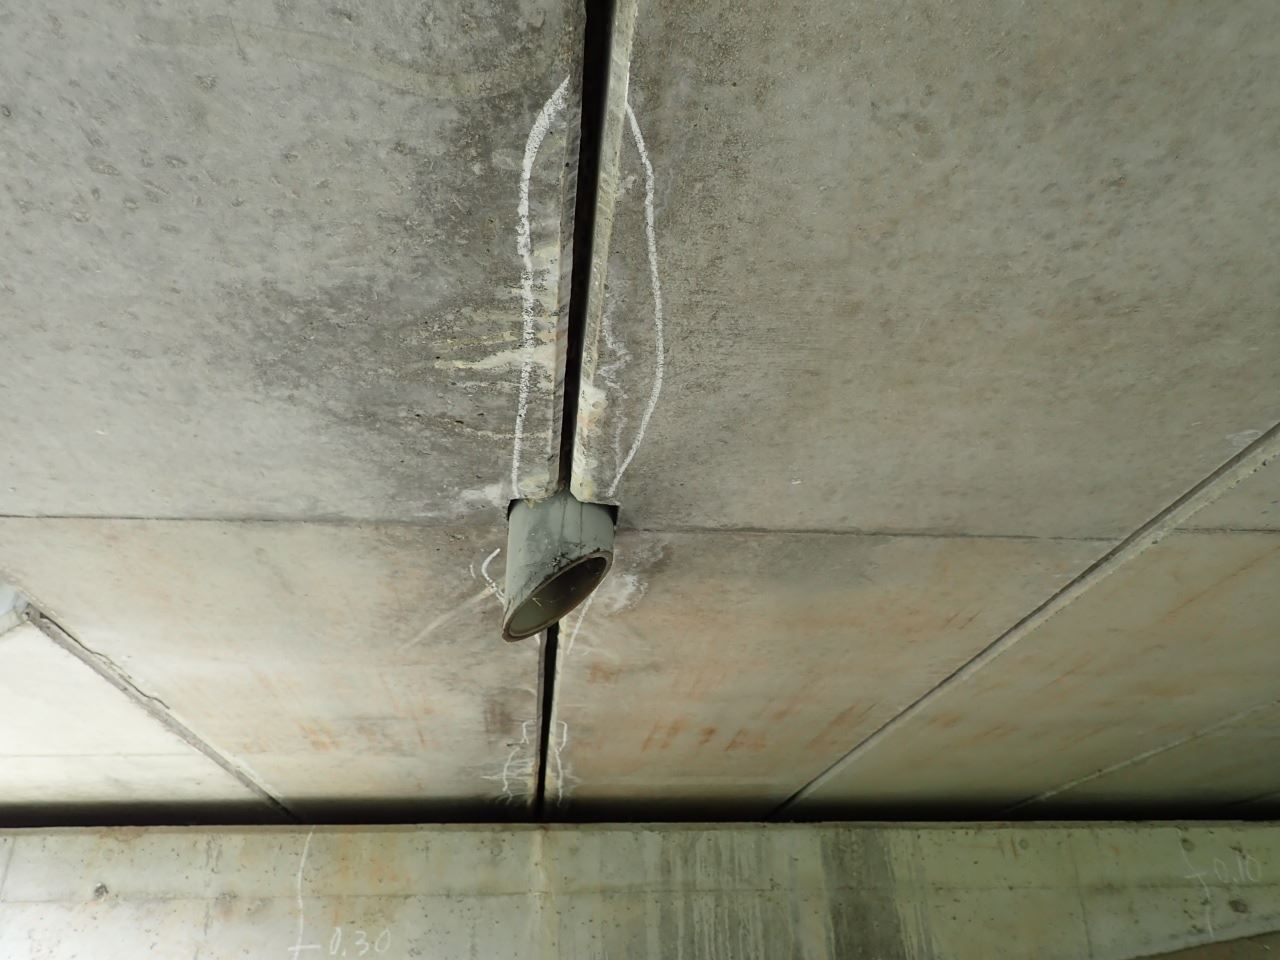
\includegraphics[width=0.675\linewidth]{figures_vlm/s8/s8_03_girder_spalling.jpg}\par}
    \vspace{2pt}
    {\scriptsize\raggedright
    \textbf{Quality Metrics:}~\textit{Sim(emb):~0.743;\enspace Priority:~1.00;\enspace Level:~5}\\[1pt]
    \textbf{GT:} \begin{CJK}{UTF8}{ipxm}{\CJKfamily{ipxg}主桁}に後埋めモルタルの剥離・鋼材露出、間詰めに一部{\CJKfamily{ipxg}錆}汁を伴う{\CJKfamily{ipxg}遊離石灰}が見られる。経過観察を行い、状況により補修を行う。\end{CJK}\\[1pt]
    \textbf{Pred:} \begin{CJK}{UTF8}{ipxm}{\CJKfamily{ipxg}主桁}にひびわれ、鉄筋露出が見られる。また、間詰め部から{\CJKfamily{ipxg}錆}汁を伴う漏水跡および{\CJKfamily{ipxg}遊離石灰}が見られる。上流側下流側ともに大きな損傷は見られず、局所的な損傷であるため，次回点検時に状況の確認を行う必要がある。\end{CJK}
    \par}
  \end{minipage}
  \hfill
  \begin{minipage}[t]{0.46\textwidth}
    {\centering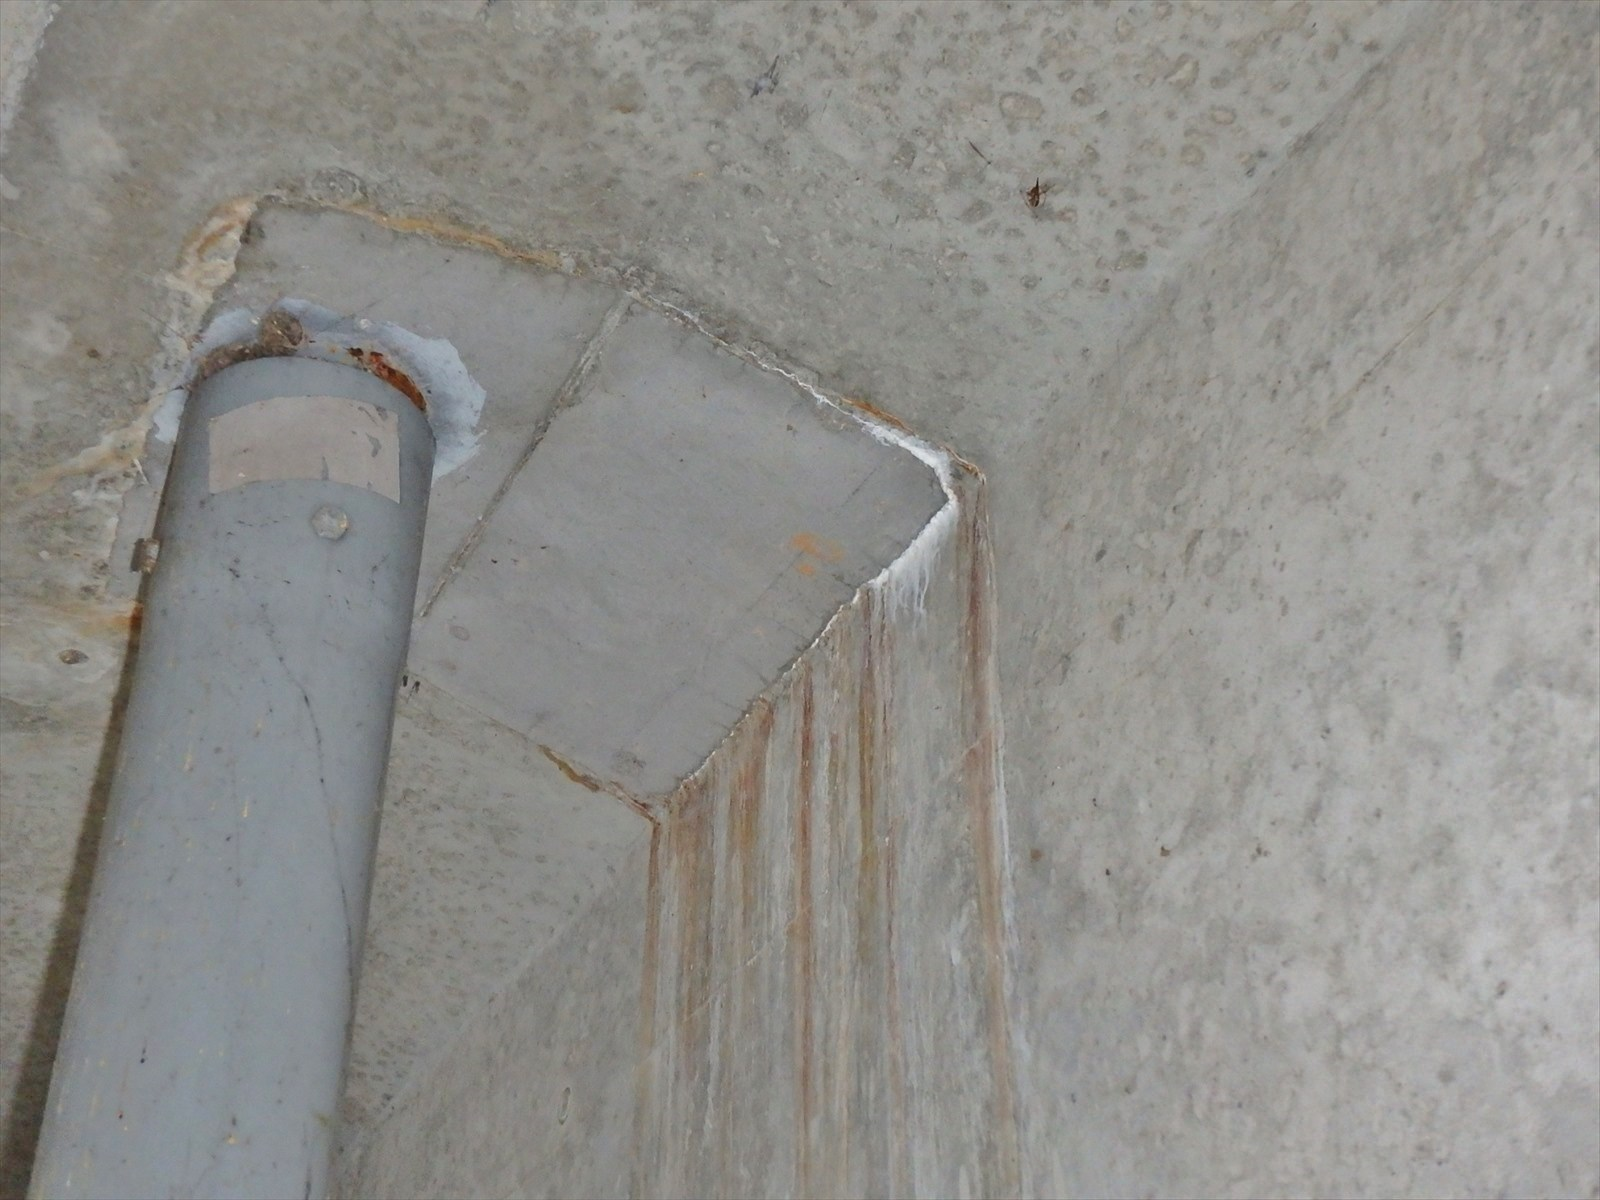
\includegraphics[width=0.675\linewidth]{figures_vlm/s8/s8_04_girder_corrosion.jpg}\par}
    \vspace{2pt}
    {\scriptsize\raggedright
    \textbf{Quality Metrics:}~\textit{Sim(emb):~0.713;\enspace Priority:~0.81;\enspace Level:~4}\\[1pt]
    \textbf{GT:} \begin{CJK}{UTF8}{ipxm}{\CJKfamily{ipxg}主桁}に{\CJKfamily{ipxg}漏水}跡（錆汁）が見られる。損傷は状況に応じて補修を行う事が望ましい。\end{CJK}\\[1pt]
    \textbf{Pred:} \begin{CJK}{UTF8}{ipxm}{\CJKfamily{ipxg}主桁}にひびわれ、鉄筋露出が見られる。また、PC床版部からの雨水伸縮が原因と思われる{\CJKfamily{ipxg}漏水}跡および滞水もみられる。車両通行時や地覆上空間からの雨水の侵入が要因と推定される。\end{CJK}
    \par}
  \end{minipage}
  \caption{Representative PASS predictions (1/3). \textbf{GT}: pairdata~v3 ground truth (Japanese); \textbf{Pred}: v0.9 DoRA~$r{=}24$ output; \textit{Sim(emb)}: 2048-dim composite cosine similarity; \textit{Priority}: scorer output; \textit{Level}: priority tier.}
  \label{fig:u73_pass_1}
\end{figure}
\clearpage

\begin{figure}[H]
  \centering
  \begin{minipage}[t]{0.46\textwidth}
    {\centering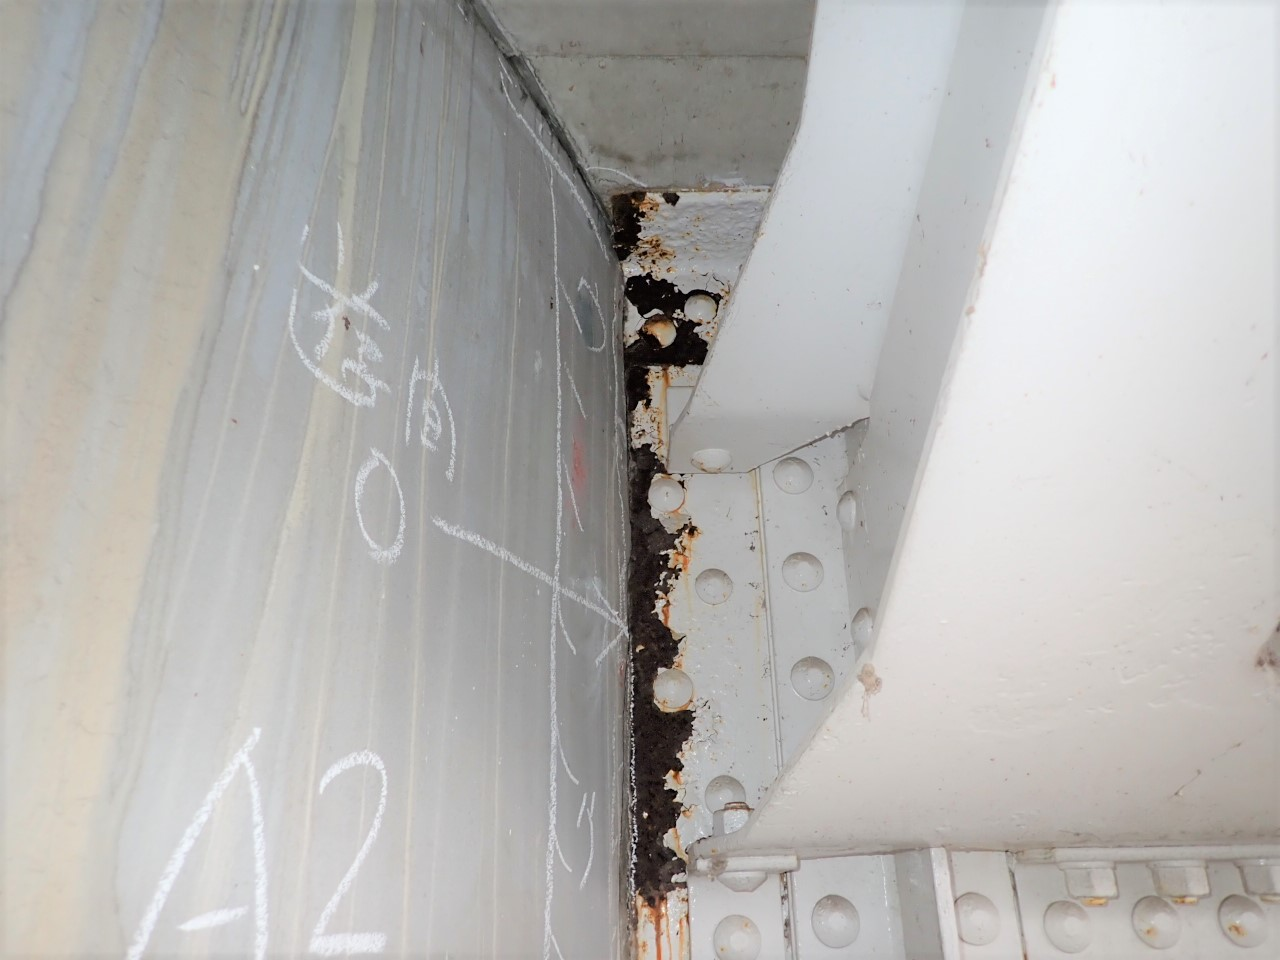
\includegraphics[width=0.675\linewidth]{figures_vlm/s8/s8_05_girder_settlement.jpg}\par}
    \vspace{2pt}
    {\scriptsize\raggedright
    \textbf{Quality Metrics:}~\textit{Sim(emb):~0.588;\enspace Priority:~0.81;\enspace Level:~4}\\[1pt]
    \textbf{GT:} \begin{CJK}{UTF8}{ipxm}伸縮装置にゴムの変形、A2橋台パラペットと{\CJKfamily{ipxg}主桁}の接触が見られる。経過観察を行い、状況により補修を行う。\end{CJK}\\[1pt]
    \textbf{Pred:} \begin{CJK}{UTF8}{ipxm}{\CJKfamily{ipxg}主桁}にひびわれ、鉄筋露出が見られる。また、間詰めから錆汁などが浸透していると思われる漏水跡も見られる。車両通行時や地覆上部の人工衛生等での立ち入りは控えるよう要望する。\end{CJK}
    \par}
  \end{minipage}
  \hfill
  \begin{minipage}[t]{0.46\textwidth}
    {\centering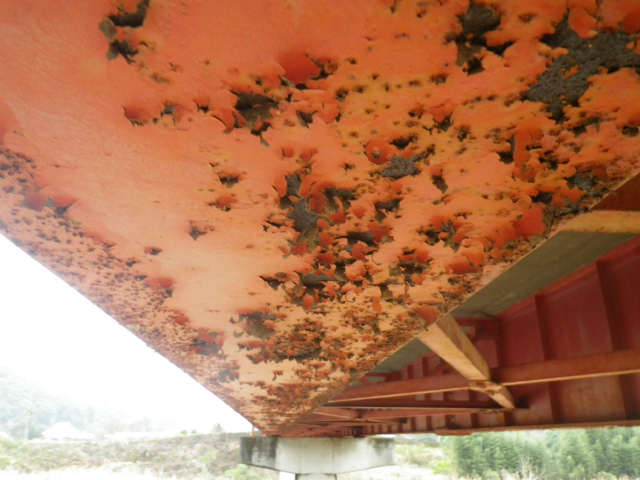
\includegraphics[width=0.675\linewidth]{figures_vlm/s8/s8_06_girder_other.jpg}\par}
    \vspace{2pt}
    {\scriptsize\raggedright
    \textbf{Quality Metrics:}~\textit{Sim(emb):~0.555;\enspace Priority:~0.81;\enspace Level:~4}\\[1pt]
    \textbf{GT:} \begin{CJK}{UTF8}{ipxm}{\CJKfamily{ipxg}主桁}・横桁に塗装剥がれや防食機能の劣化が認められる\end{CJK}\\[1pt]
    \textbf{Pred:} \begin{CJK}{UTF8}{ipxm}{\CJKfamily{ipxg}主桁}にひびわれ、鉄筋露出が見られる。また、PC床版部からの雨水等により、床版下部と間詰め部分で遊離石灰が生じており、目地に漏水跡が見られる。車両通行時の視線や近づきは控える必要がある。\end{CJK}
    \par}
  \end{minipage}
  \\[4pt]
  \begin{minipage}[t]{0.46\textwidth}
    {\centering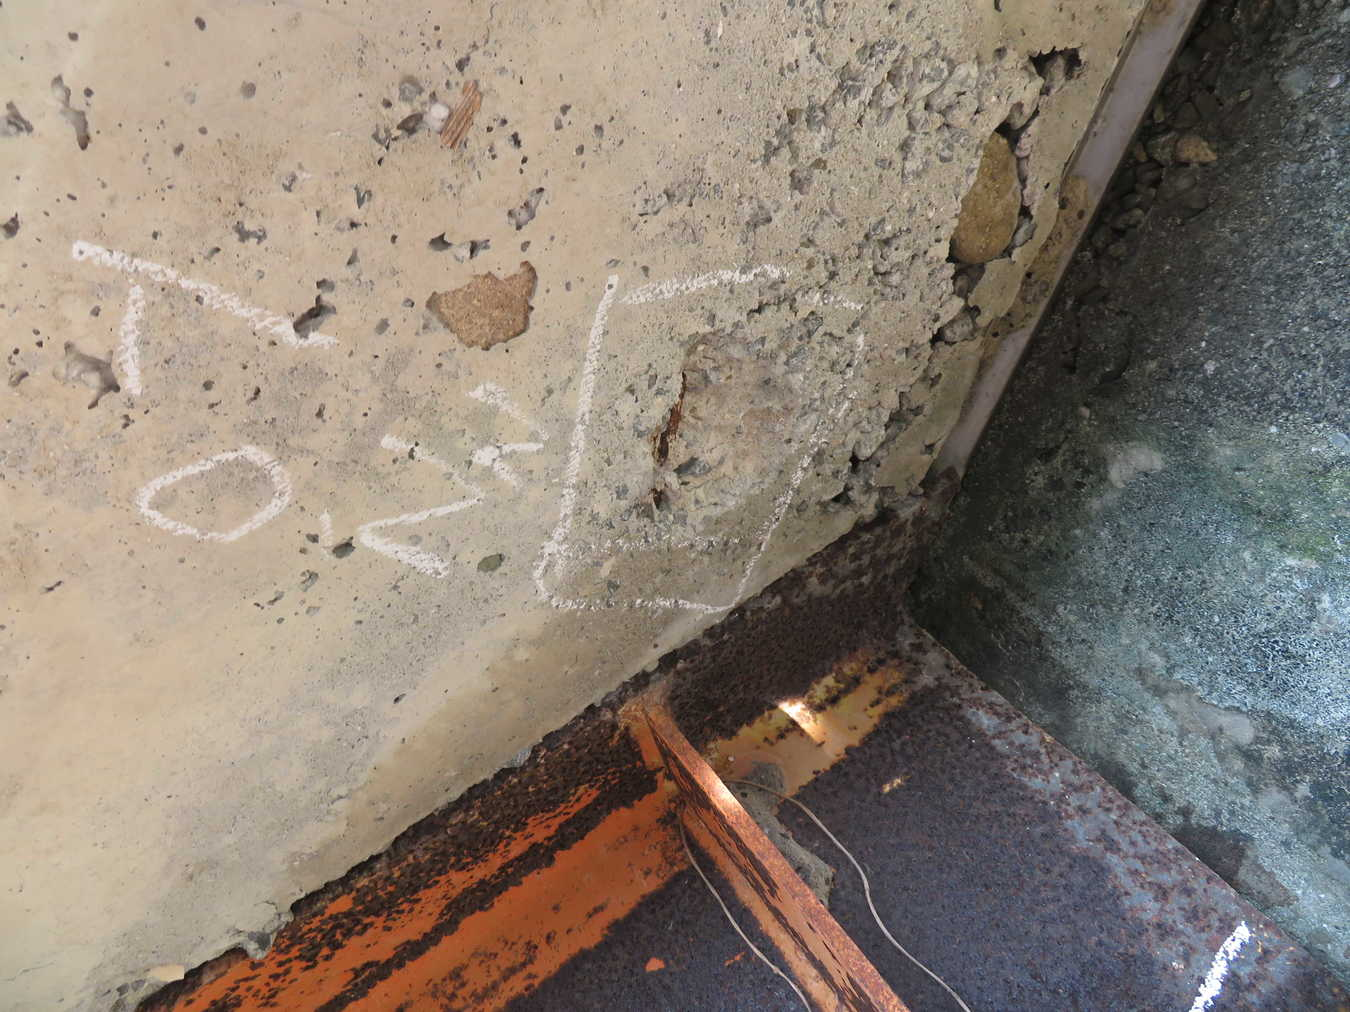
\includegraphics[width=0.675\linewidth]{figures_vlm/s8/s8_07_slab_cracking.jpg}\par}
    \vspace{2pt}
    {\scriptsize\raggedright
    \textbf{Quality Metrics:}~\textit{Sim(emb):~0.824;\enspace Priority:~0.81;\enspace Level:~4}\\[1pt]
    \textbf{GT:} \begin{CJK}{UTF8}{ipxm}・{\CJKfamily{ipxg}床版}に乾燥収縮によるものと推測される{\CJKfamily{ipxg}ひびわれ}、鉄筋の{\CJKfamily{ipxg}腐食}膨張によるものと推測される{\CJKfamily{ipxg}うき}、鉄筋のかぶり不足による{\CJKfamily{ipxg}鉄筋露出}が見られる。また、橋面からの浸透水によるものと推測される遊離石灰が見られる。\end{CJK}\\[1pt]
    \textbf{Pred:} \begin{CJK}{UTF8}{ipxm}主桁に{\CJKfamily{ipxg}ひびわれ}、{\CJKfamily{ipxg}鉄筋露出}が見られる。また、間詰めから錆汁などが浸透し、内部鉄筋が{\CJKfamily{ipxg}腐食}していると推定される。{\CJKfamily{ipxg}床版}には{\CJKfamily{ipxg}うき}および{\CJKfamily{ipxg}鉄筋露出}が見られる。道路橋の機能に支障が生じていないため、次回点検時に状況の確認を行う。\end{CJK}
    \par}
  \end{minipage}
  \hfill
  \begin{minipage}[t]{0.46\textwidth}
    {\centering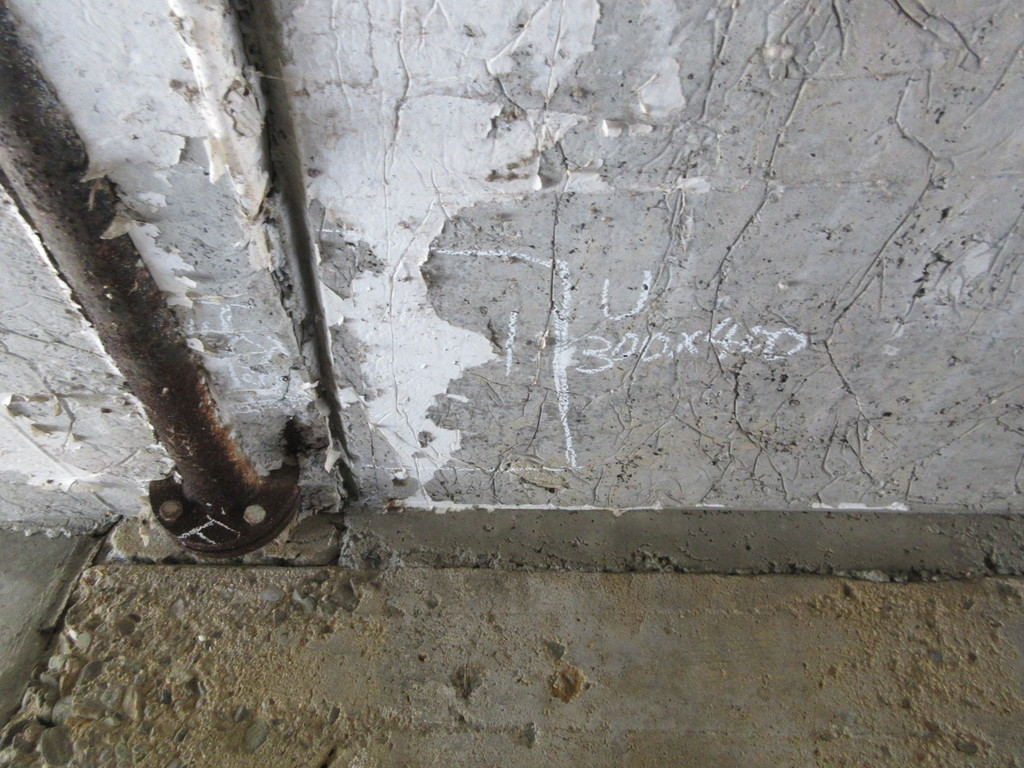
\includegraphics[width=0.675\linewidth]{figures_vlm/s8/s8_08_slab_rebar_exposure.jpg}\par}
    \vspace{2pt}
    {\scriptsize\raggedright
    \textbf{Quality Metrics:}~\textit{Sim(emb):~0.774;\enspace Priority:~0.81;\enspace Level:~4}\\[1pt]
    \textbf{GT:} \begin{CJK}{UTF8}{ipxm}床版にうき、{\CJKfamily{ipxg}鉄筋露出}、{\CJKfamily{ipxg}遊離石灰}が見られる。うき・{\CJKfamily{ipxg}鉄筋露出}は、被り不足や中性化が原因と考えられる。損傷は、局所的であるため、次回点検時に状況の確認を行う。\end{CJK}\\[1pt]
    \textbf{Pred:} \begin{CJK}{UTF8}{ipxm}主桁にひびわれ、{\CJKfamily{ipxg}鉄筋露出}が見られる。また、間詰め部から錆汁を伴う漏水跡および{\CJKfamily{ipxg}遊離石灰}が見られる。車両通行時や近ヘッドマインダーでの被り不足が原因と思われる。次回点検時に進行度を確認する必要がある。\end{CJK}
    \par}
  \end{minipage}
  \caption{Representative PASS predictions (2/3). \textbf{GT}: pairdata~v3 ground truth (Japanese); \textbf{Pred}: v0.9 DoRA~$r{=}24$ output; \textit{Sim(emb)}: 2048-dim composite cosine similarity; \textit{Priority}: scorer output; \textit{Level}: priority tier.}
  \label{fig:u73_pass_2}
\end{figure}
\clearpage

\begin{figure}[H]
  \centering
  \begin{minipage}[t]{0.46\textwidth}
    {\centering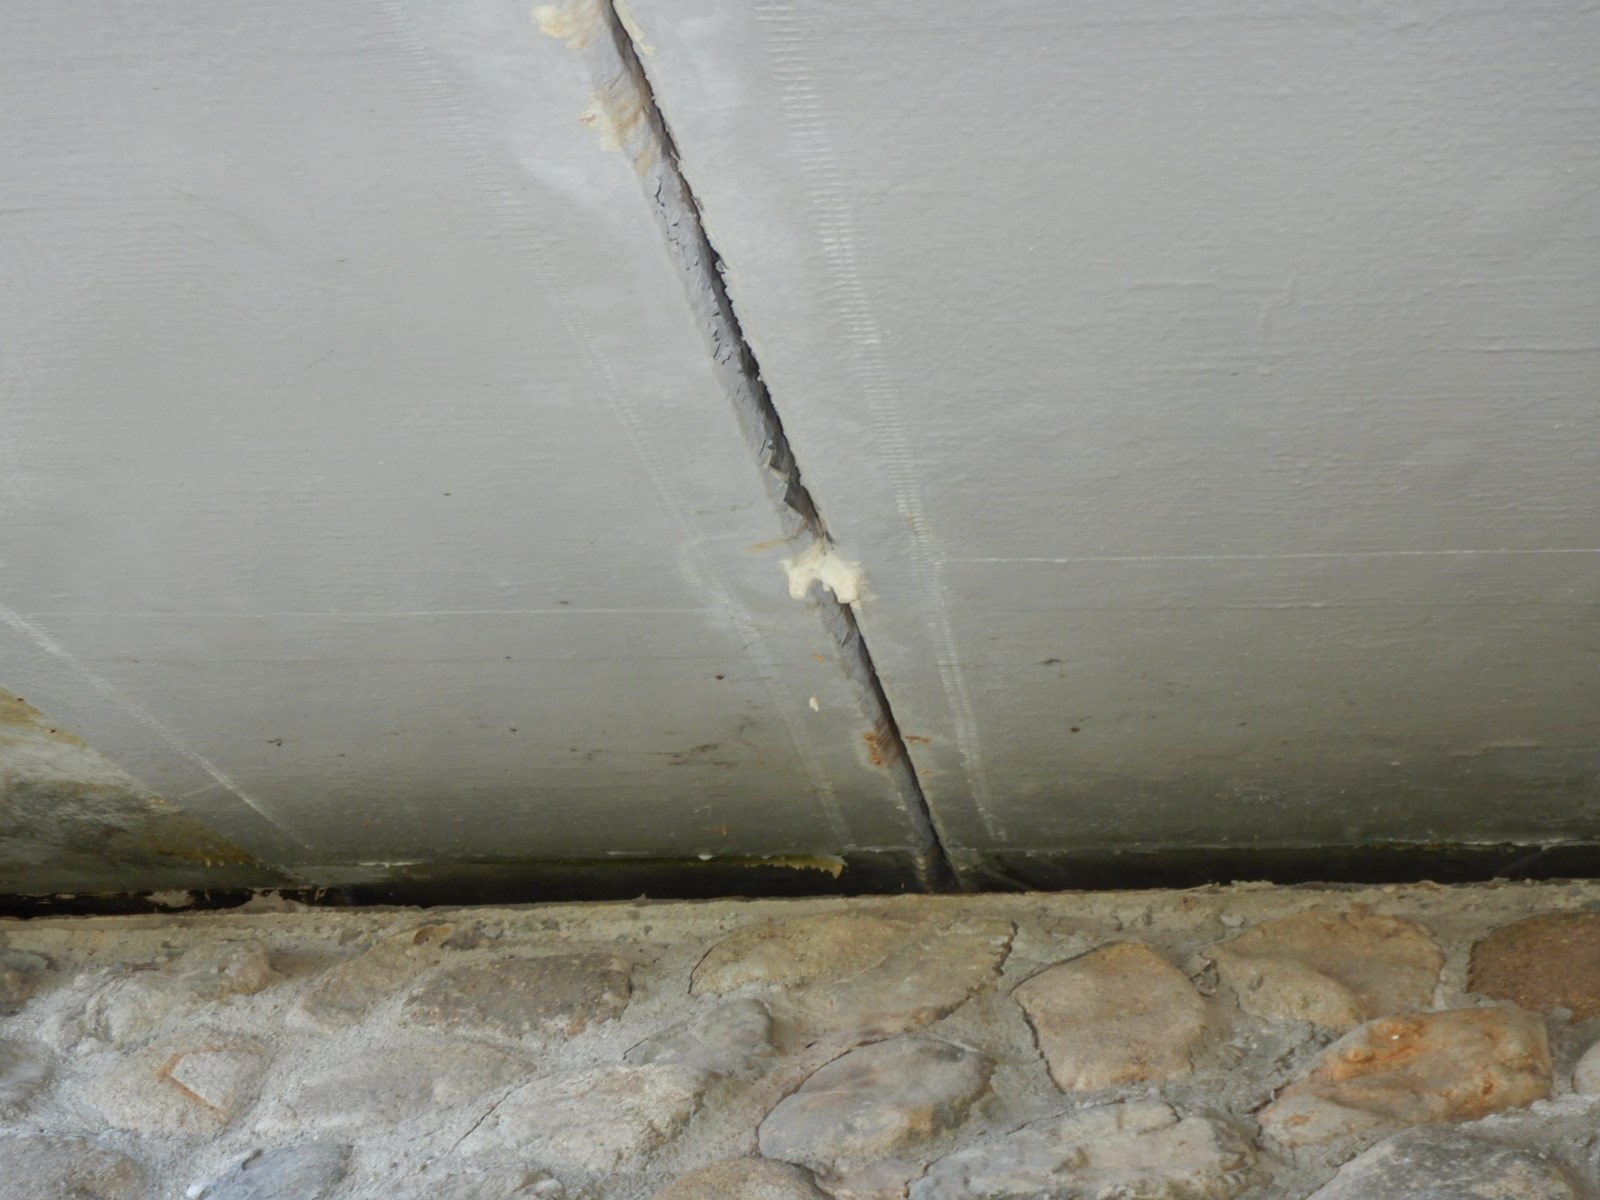
\includegraphics[width=0.675\linewidth]{figures_vlm/s8/s8_09_slab_corrosion.jpg}\par}
    \vspace{2pt}
    {\scriptsize\raggedright
    \textbf{Quality Metrics:}~\textit{Sim(emb):~0.603;\enspace Priority:~0.81;\enspace Level:~4}\\[1pt]
    \textbf{GT:} \begin{CJK}{UTF8}{ipxm}{\CJKfamily{ipxg}床版}間詰め部から遊離石灰（錆汁）が見られる。損傷は状況に応じて補修を行う事が望ましい。\end{CJK}\\[1pt]
    \textbf{Pred:} \begin{CJK}{UTF8}{ipxm}主桁にひびわれ、鉄筋露出が見られる。また、PC{\CJKfamily{ipxg}床版}部からの雨水伸縮が原因と思われる漏水跡および滞水もみられる。車両通行時の視線はほとんどなく、その他の方向での視点であれば、道路橋の機能に支障は生じていない。\end{CJK}
    \par}
  \end{minipage}
  \hfill
  \begin{minipage}[t]{0.46\textwidth}
    {\centering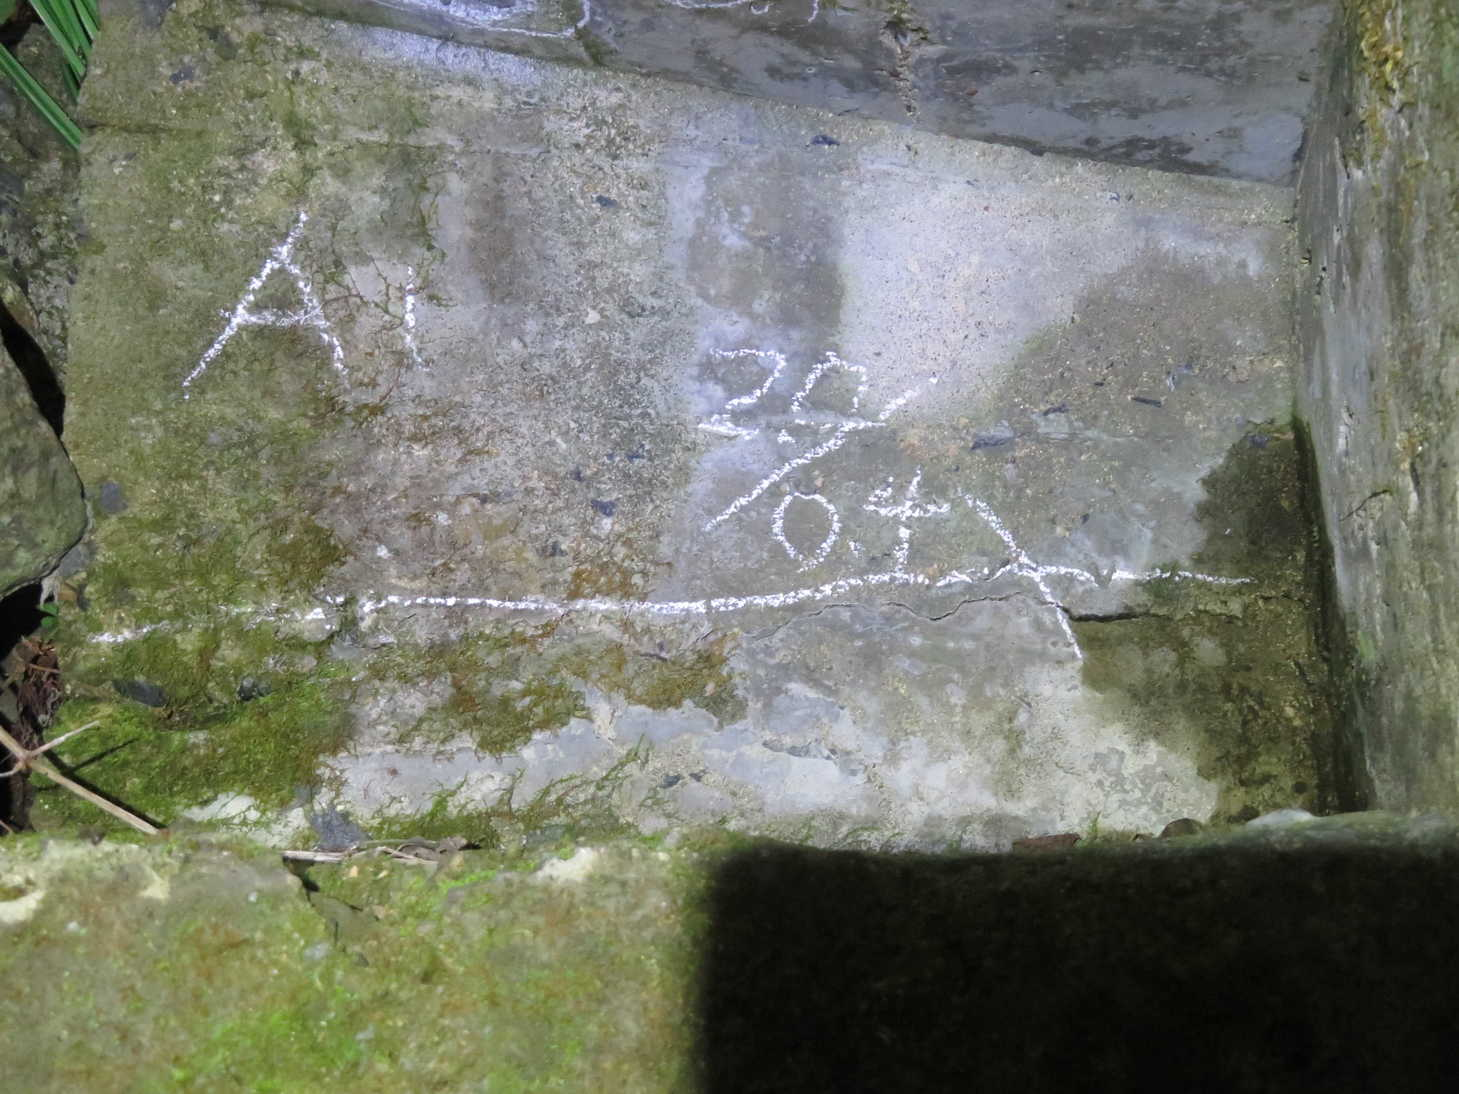
\includegraphics[width=0.675\linewidth]{figures_vlm/s8/s8_10_abutment_cracking.jpg}\par}
    \vspace{2pt}
    {\scriptsize\raggedright
    \textbf{Quality Metrics:}~\textit{Sim(emb):~0.778;\enspace Priority:~0.81;\enspace Level:~4}\\[1pt]
    \textbf{GT:} \begin{CJK}{UTF8}{ipxm}・橋台に施工不良による{\CJKfamily{ipxg}ひびわれ}（コールドジョイント）および鉄筋のかぶり不足による{\CJKfamily{ipxg}鉄筋露出}が見られる。また、伸縮装置部からの{\CJKfamily{ipxg}漏水}による{\CJKfamily{ipxg}漏水}跡およびすりへりが見られる。\end{CJK}\\[1pt]
    \textbf{Pred:} \begin{CJK}{UTF8}{ipxm}主桁に{\CJKfamily{ipxg}ひびわれ}、{\CJKfamily{ipxg}鉄筋露出}が見られる。また、PC床版部からの雨水伸縮が原因と思われる{\CJKfamily{ipxg}漏水}跡および表面劣化（剥離）が見られる。車両通行時の視線や近づきは控えめにする必要がある。\end{CJK}
    \par}
  \end{minipage}
  \\[4pt]
  \begin{minipage}[t]{0.46\textwidth}
    {\centering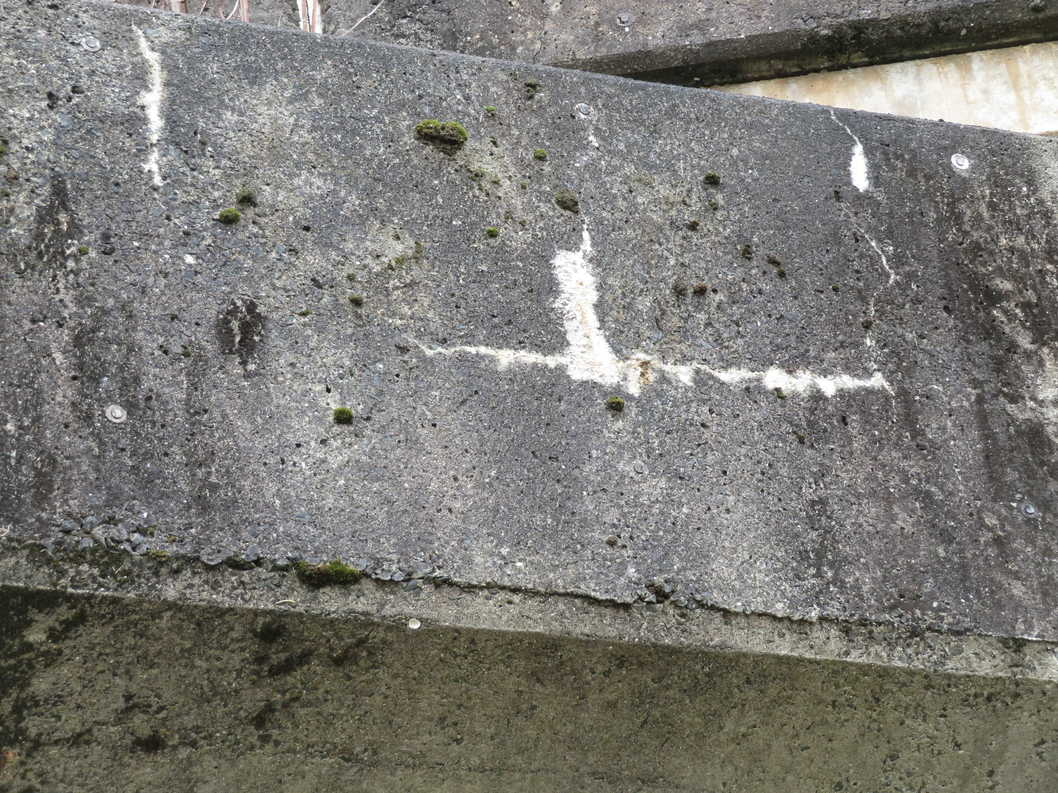
\includegraphics[width=0.675\linewidth]{figures_vlm/s8/s8_11_abutment_rebar_exposure.jpg}\par}
    \vspace{2pt}
    {\scriptsize\raggedright
    \textbf{Quality Metrics:}~\textit{Sim(emb):~0.690;\enspace Priority:~0.81;\enspace Level:~4}\\[1pt]
    \textbf{GT:} \begin{CJK}{UTF8}{ipxm}・橋脚に鉄筋の腐食膨張によるものと推測されるうきおよび鉄筋のかぶり不足による{\CJKfamily{ipxg}鉄筋露出}がみられる。また、橋面からの浸透水によるものと推測される軽微{\CJKfamily{ipxg}遊離石灰}が見られる。・橋台に伸縮装置部からの漏水による漏水跡が見られる。\end{CJK}\\[1pt]
    \textbf{Pred:} \begin{CJK}{UTF8}{ipxm}主桁にひびわれ、{\CJKfamily{ipxg}鉄筋露出}が見られる。また、PC床版部からの雨水等により、床版下部と間詰め部分で{\CJKfamily{ipxg}遊離石灰}が生じており、進行性は否定的である。\end{CJK}
    \par}
  \end{minipage}
  \hfill
  \begin{minipage}[t]{0.46\textwidth}
    {\centering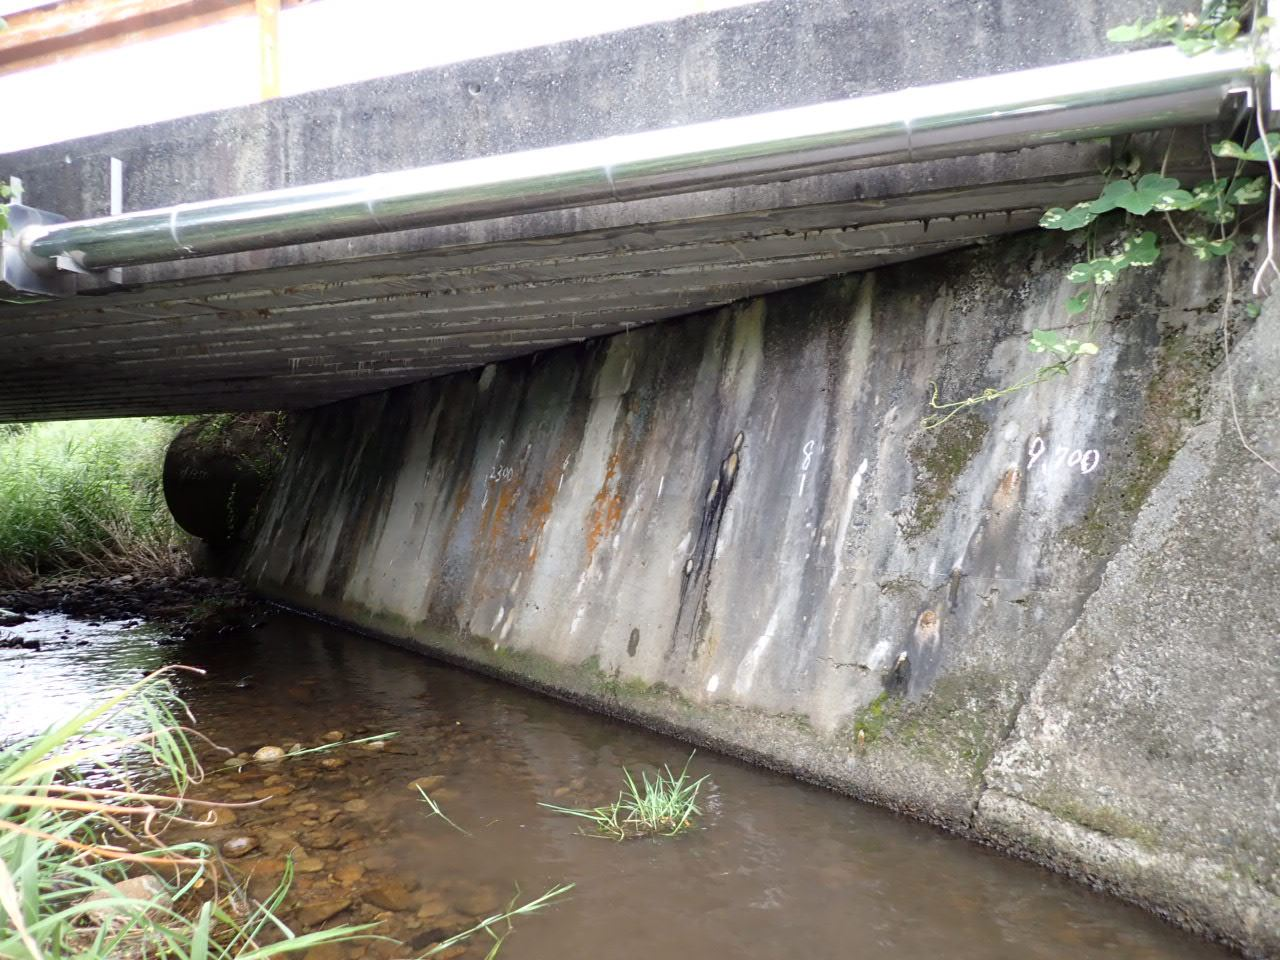
\includegraphics[width=0.675\linewidth]{figures_vlm/s8/s8_12_abutment_spalling.jpg}\par}
    \vspace{2pt}
    {\scriptsize\raggedright
    \textbf{Quality Metrics:}~\textit{Sim(emb):~0.662;\enspace Priority:~0.81;\enspace Level:~4}\\[1pt]
    \textbf{GT:} \begin{CJK}{UTF8}{ipxm}橋台に{\CJKfamily{ipxg}うき}、漏水がみられる。漏水は{\CJKfamily{ipxg}伸縮装置}から浸入したものと考えられる。緊急性はなく、予防保全の観点から健全度評価「Ⅱ」とする。\end{CJK}\\[1pt]
    \textbf{Pred:} \begin{CJK}{UTF8}{ipxm}主桁にひびわれ、{\CJKfamily{ipxg}うき}が見られる。また、鉄筋露出も見られる。上流側{\CJKfamily{ipxg}伸縮装置}からの浸透水と思われる。道路橋の機能に支障は生じており、次回点検時に進行度を判断する必要がある。\end{CJK}
    \par}
  \end{minipage}
  \caption{Representative PASS predictions (3/3). \textbf{GT}: pairdata~v3 ground truth (Japanese); \textbf{Pred}: v0.9 DoRA~$r{=}24$ output; \textit{Sim(emb)}: 2048-dim composite cosine similarity; \textit{Priority}: scorer output; \textit{Level}: priority tier.}
  \label{fig:u73_pass_3}
\end{figure}

%%--------------------------------------------------------------------
\subsection*{U.7.4\quad Damage VLM Apps v1.0.0 Test Prediction: $n{=}10{,}903$}
\label{sec:u74_v10_prediction}
%%--------------------------------------------------------------------

\subsubsection*{Overview}

Following the DoRA $r{=}24$ model selection described in Section~\ref{sec:u8_dora},
we deployed the merged adapter (\path{llava_v09_dora_r24_merged}) in a
full-dataset inference pipeline (v1.0.0) over all $n{=}10{,}903$ records of the
Rank\_c image--text dataset.
This experiment serves as the final end-to-end system test,
verifying that the Quality Guard and Priority Scoring modules operate correctly
at production scale.

\subsubsection*{Inference Configuration}

\begin{itemize}
  \item \textbf{Model:} LLaVA-1.5-7B + DoRA $r{=}24$ merged adapter
        (\path{llava_v09_dora_r24_merged}), 4-bit quantisation
        (BitsAndBytesConfig, NF4)
  \item \textbf{Framework:} \texttt{transformers} (LlavaForConditionalGeneration),
        PEFT, PyTorch
  \item \textbf{Batch size:} 4 images per forward pass
  \item \textbf{Checkpoint interval:} every 2{,}000 records
  \item \textbf{Image resolution:} $336 \times 336$\,px
  \item \textbf{Execution period:} 2026-06-02 20:20 -- 2026-06-03 06:53 (JST)
\end{itemize}

\subsubsection*{Results}

Table~\ref{tab:u74_inference_results} summarises the Quality Guard outcomes
and Priority Level distribution for all $n{=}10{,}903$ predictions.

\begin{table}[H]
  \centering
  \caption{v1.0.0 full-dataset inference results ($n{=}10{,}903$).}
  \label{tab:u74_inference_results}
  \begin{tabular}{lrr}
    \toprule
    \textbf{Metric} & \textbf{Count} & \textbf{Ratio (\%)} \\
    \midrule
    Total records                & 10{,}903 & 100.0 \\
    \addlinespace
    Quality Guard PASS           & 10{,}668 &  97.8 \\
    Quality Guard FAIL           &       0  &   0.0 \\
    Missing (no image)           &     235  &   2.2 \\
    \addlinespace
    Priority Level~3             &     454  &   4.3 \\
    Priority Level~4             &   9{,}185 &  86.1 \\
    Priority Level~5             &   1{,}029 &   9.6 \\
    \addlinespace
    Total processing time        & \multicolumn{2}{c}{10.55\,h (37{,}968\,s)} \\
    Mean processing speed        & \multicolumn{2}{c}{3.5\,s / image} \\
    \bottomrule
  \end{tabular}
\end{table}

The Quality Guard PASS rate of 97.8\,\% at production scale
is consistent with the validation-set rate observed during training
(Section~\ref{sec:u6_quality_guard}).
No FAIL outputs were recorded, confirming that the v0.9 DoRA $r{=}24$ model
does not generate malformed or structurally invalid text under the full
distribution of bridge damage imagery.
The 2.2\,\% missing rate corresponds exclusively to records lacking an
associated image file and is unrelated to model quality.

Priority Level~4 dominates at 86.1\,\%, consistent with the dataset's
focus on moderate structural damage.
Level~5 (9.6\,\%) captures severe or multi-damage patterns,
while Level~3 (4.3\,\%) identifies minor damage cases.
The batch-size-4 processing strategy achieved a mean throughput of
3.5\,s/image---a 50\,\% improvement over single-image inference---enabling
the full $n{=}10{,}903$ run to complete within 10.55\,h on a single consumer GPU.

The final predictions are stored in
\path{data/v10_full/v10_full_r24_dora.xlsx} (10{,}903 rows),
which serves as the primary output for downstream structural health
monitoring applications.

\subsubsection*{Structural Member and Damage Type Analysis}

Figure~\ref{fig:u74_member_damage} presents the member frequency,
damage type frequency, and member$\times$damage co-occurrence heatmap
for all PASS predictions ($n{=}10{,}668$).
The analysis follows the same keyword-extraction methodology used in
Section~\ref{sec:u6_quality_guard} and Figure~21.

\begin{figure}[H]
  \centering
  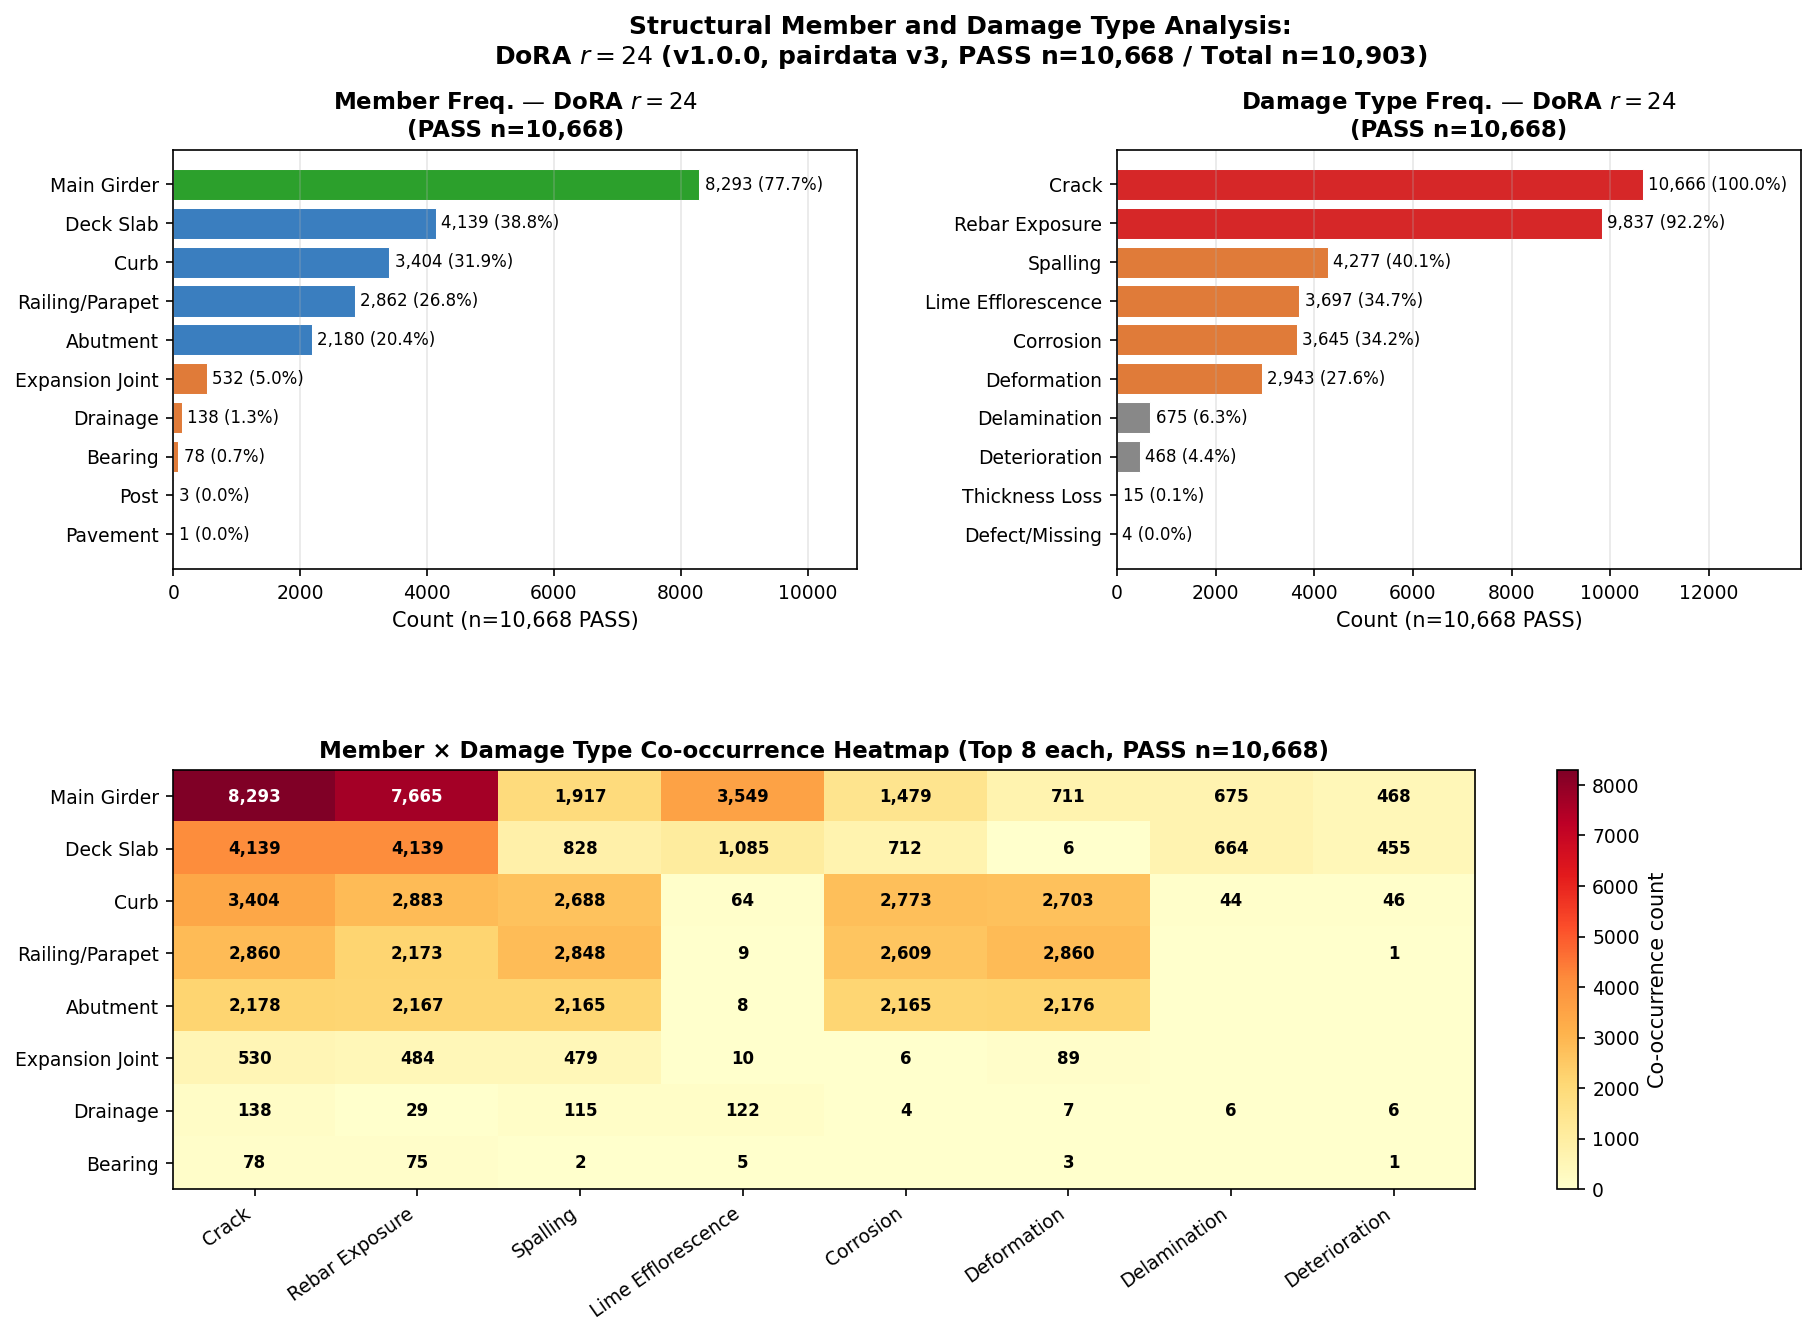
\includegraphics[width=\linewidth]{figures_vlm/u74_member_damage_analysis.png}
  \caption{Structural member and damage type analysis for v1.0.0 full-dataset
    PASS predictions ($n{=}10{,}668$).
    \textit{Top-left}: structural member mention frequency;
    \textit{Top-right}: damage type frequency;
    \textit{Bottom}: member $\times$ damage type co-occurrence heatmap (top 8 each).
    Model: DoRA $r{=}24$ (v1.0.0, pairdata v3).}
  \label{fig:u74_member_damage}
\end{figure}

\paragraph{Member frequency.}
Main Girder dominates at 77.7\,\% ($n{=}8{,}293$), reflecting the
dataset composition in which girder-type bridges represent the majority
of inspected structures.
Deck Slab (38.8\,\%), Curb (31.9\,\%), and Railing/Parapet (26.8\,\%)
form the next tier.
Abutment (20.4\,\%) is the only substructure member appearing frequently,
consistent with the dataset's primary focus on superstructure inspections.

\paragraph{Damage type frequency.}
Crack appears in virtually all PASS predictions (100.0\,\%),
and Rebar Exposure in 92.2\,\%, indicating that the model has learned to
identify the two most prevalent deterioration modes in the training corpus.
Spalling (40.1\,\%), Lime Efflorescence (34.7\,\%), and Corrosion (34.2\,\%)
occupy an intermediate tier, while Deformation (27.6\,\%) is predominantly
associated with curbs and railings.

\paragraph{Member $\times$ damage co-occurrence.}
The heatmap reveals distinct member--damage association patterns:
\begin{itemize}
  \item \textbf{Main Girder} co-occurs with Crack (8{,}293; 100\,\%)
        and Rebar Exposure (7{,}665; 92.4\,\%), confirming the model's
        consistent recognition of flexural cracking and section loss
        in the primary load-carrying element.
  \item \textbf{Deck Slab} co-occurs with both Crack and Rebar Exposure
        at 100\,\% ($n{=}4{,}139$), reflecting the combined effect of
        wheel-load fatigue and chloride-induced corrosion in slab elements.
  \item \textbf{Curb} and \textbf{Railing/Parapet} exhibit high co-occurrence
        with Corrosion ($>$80\,\%) and Deformation ($>$79\,\%),
        capturing steel-section loss and geometric distortion typical of
        exposed barrier elements.
  \item \textbf{Abutment} co-occurs with Rebar Exposure and Crack at
        nearly 100\,\%, consistent with carbonation-induced corrosion
        mechanisms common in concrete substructures.
\end{itemize}

These patterns are consistent with physical knowledge of bridge deterioration
and corroborate that the DoRA $r{=}24$ model generalises the damage-recognition
patterns learned on the 2{,}500-sample pairdata~v3 corpus to the full
$n{=}10{,}903$ field dataset without systematic mode collapse or
spurious damage attribution.

%%--------------------------------------------------------------------
\subsection*{U.8 DoRA vs.\ LoRA Comparison (v0.9, pairdata v3)}
\label{sec:u8_dora}
%%--------------------------------------------------------------------

\subsubsection*{U.8.1\enspace DoRA Motivation and Formulation}

The LoRA rank ablation in Section~\ref{sec:u4_training} identifies $r=64$
as the optimal rank for the v0.8 QLoRA baseline on pairdata\_v3,
achieving the lowest eval loss of $3.122$ and a token accuracy of
$98.90$\,\% at epoch~2.421.
The ablation further established that the $168.8$\,M trainable parameters
at $r=64$ (4.56\,\% of the 7B backbone) are necessary to capture the
fine-grained correspondence between complex damage imagery and structured
recognition text---a bandwidth that narrower adapters ($r\le32$) cannot
provide.

Building on this finding, U.8 investigates the following research questions
under the same $r=64$ regime:
\begin{enumerate}[label=(\roman*)]
  \item \textbf{Validation loss.} Does decomposing weight updates into an
        explicit \emph{direction} component and a \emph{magnitude} component
        (DoRA) yield a lower best-checkpoint eval loss than vanilla LoRA at
        the same rank and VRAM budget?
  \item \textbf{Cosine similarity.} Does the finer gradient control
        afforded by magnitude--direction separation improve the semantic
        alignment between predicted descriptions and pairdata\_v3
        ground-truth annotations, as measured by the 2{,}048-dimensional
        composite cosine evaluator?
  \item \textbf{Hallucination.} Does DoRA's implicit regularisation via
        column-wise $\ell_2$ normalisation reduce the generation of
        hallucinated measurement values (Category~C noise) and
        ungrounded platitude sentences (Category~B noise) on the
        fixed $n{=}800$ test set?
\end{enumerate}

To investigate whether a structurally different low-rank adaptation method
can improve quality within the same 16\,GB VRAM budget,
we evaluate \textbf{DoRA}
(Weight-Decomposed Low-Rank Adaptation; Liu et al.~\cite{liu2024dora}).

DoRA decomposes the pretrained weight matrix $W_0$ into a magnitude
component $m$ and a directional component $V$:
\[
  W = m \cdot \frac{V + \Delta V}{\|V + \Delta V\|_c},
  \quad
  \Delta V = B A,
\]
where $B \in \mathbb{R}^{d \times r}$, $A \in \mathbb{R}^{r \times k}$
are the same low-rank factors as in LoRA, and $\|\cdot\|_c$ denotes
column-wise $\ell_2$ normalisation.
By training both $m$ and $\Delta V$ while keeping the direction normalised,
DoRA achieves higher expressive power at the same rank and parameter count
as vanilla LoRA, without requiring additional VRAM.

For the bridge damage inspection domain specifically, three properties make
DoRA attractive:
\begin{itemize}
  \item \textbf{Low-entropy target distribution.}
        Japanese damage descriptions follow constrained vocabularies and
        stereotyped syntactic patterns.
        The direction--magnitude decomposition provides finer gradient
        control over specialised tokens, improving vocabulary recall.
  \item \textbf{Small dataset ($n{=}2{,}500$) robustness.}
        Magnitude normalisation acts as an implicit regulariser, reducing
        overfitting risk on the limited training corpus.
  \item \textbf{Compatibility with 4-bit NF4 quantisation.}
        DoRA operates entirely in the adapter weight space, so it is fully
        compatible with the QLoRA (BitsAndBytes NF4) quantisation used
        throughout v0.8 training.
\end{itemize}

\paragraph{Mathematical Formulation.}

\paragraph{LoRA baseline.}
Given a pretrained weight matrix $W_0 \in \mathbb{R}^{d \times k}$,
LoRA parameterises the update as:
\[
  W_{\text{LoRA}} = W_0 + \Delta W, \quad
  \Delta W = B A,
\]
where $B \in \mathbb{R}^{d \times r}$ and $A \in \mathbb{R}^{r \times k}$
are low-rank factors ($r \ll \min(d, k)$),
initialised as $B = 0$, $A \sim \mathcal{N}(0, \sigma^2)$.
Only $\{B, A\}$ are trained; $W_0$ is frozen.

\paragraph{DoRA weight decomposition.}
DoRA first decomposes $W_0$ in polar form
(column-wise magnitude--direction factorisation):
\[
  W_0 = m \cdot V_0,
  \quad
  m = \|W_0\|_c \in \mathbb{R}^{1 \times k},
  \quad
  V_0 = \frac{W_0}{\|W_0\|_c},
\]
where $\|\cdot\|_c$ denotes the column-wise $\ell_2$ norm
(each column of $V_0$ has unit $\ell_2$ norm).
$m$ is a learnable vector; $V_0$ is the normalised direction of $W_0$.

\paragraph{DoRA update rule.}
DoRA learns a low-rank directional perturbation $\Delta W = BA$
and simultaneously scales the result with the learned magnitude:
\[
  W_{\text{DoRA}}
  = \underbrace{m}_{\text{learned}}
    \cdot
    \underbrace{\frac{W_0 + \Delta W}{\|W_0 + \Delta W\|_c}}_{\text{normalised direction}},
  \qquad
  \Delta W = BA.
\]
Trainable parameters are $\theta = \{B, A, m\}$.
The extra cost of $m$ is $k$ scalars per weight matrix,
which is negligible compared with the $dr + rk$ parameters of $\{B, A\}$
(for LLaVA-1.5-7B at $r=32$: $|m| / (|B|+|A|) < 0.1\,\%$).

\paragraph{Comparison of trainable parameters.}
\[
  |\theta_{\text{LoRA}}| = dr + rk, \qquad
  |\theta_{\text{DoRA}}| = dr + rk + k \approx |\theta_{\text{LoRA}}|.
\]
Both adapt the same 7 target modules
(\texttt{q/k/v/o/gate\_proj/up\_proj/down\_proj});
the total VRAM footprint is therefore identical.

\paragraph{Gradient flow perspective.}
In vanilla LoRA the effective weight gradient $\nabla_{W}\mathcal{L}$
is constrained to the span of the low-rank factors.
DoRA's magnitude--direction decomposition yields two decoupled gradient paths:
\begin{enumerate}[label=(\roman*)]
  \item $\nabla_{m}\mathcal{L}$: adjusts the \emph{scale} of each output column
        independently, enabling large domain-shift corrections
        (e.g.\ Japanese technical vocabulary scaling).
  \item $\nabla_{B}\mathcal{L},\,\nabla_{A}\mathcal{L}$:
        adjusts the \emph{direction} within the low-rank subspace,
        capturing fine-grained syntactic and semantic shifts.
\end{enumerate}
This decoupled gradient signal has been shown empirically to reduce
the number of training steps required to reach a given loss level,
and to improve final accuracy on specialised downstream tasks~\cite{liu2024dora}.

%%------------------------------------------------------------------
\subsubsection*{U.8.2\enspace DoRA Training Results}
%%------------------------------------------------------------------

\paragraph{Configuration.}

All hyperparameters are held fixed to the v0.8 $r=64$ baseline
(Table~\ref{tab:u4_config}); only the adapter type is changed.

\begin{table}[h]
\centering
\caption{DoRA vs.\ LoRA configuration comparison
         (v0.9, pairdata\_v3, 2\,500-sample scale, RTX~4060~Ti~16\,GB).}
\label{tab:u8_config}
\small
\begin{tabular}{lll}
\toprule
\textbf{Parameter} & \textbf{QLoRA r\,=\,64 (v0.8)} & \textbf{QDoRA r\,=\,64 (v0.9)} \\
\midrule
Adapter type     & LoRA                 & DoRA (\texttt{use\_dora=True}) \\
Rank ($r$)       & 64                   & 64 \\
Alpha ($\alpha$) & 128 (=\,2r)          & 128 (=\,2r) \\
Dropout          & 0.05                 & 0.05 \\
Target modules   & q/k/v/o/gate/up/down & q/k/v/o/gate/up/down \\
Quantisation     & 4-bit NF4, double quant & 4-bit NF4, double quant \\
Batch / grad-acc & 4 / 4 (eff.\ 16)    & 4 / 4 (eff.\ 16) \\
Learning rate    & $2\times10^{-4}$     & $2\times10^{-4}$ \\
LR schedule      & cosine               & cosine \\
Epochs           & 3                    & 3 \\
Precision        & BF16                 & BF16 \\
Script           & \texttt{train\_v08\_qlora.py} & \texttt{train\_v09\_dora.py} \\
Output dir       & \texttt{llava\_v08\_r64\_2500} & \texttt{llava\_v09\_dora\_r64\_2500} \\
\midrule
\multicolumn{3}{l}{\textit{Implementation note: only \texttt{LoraConfig(use\_dora=True)} differs from v0.8.}} \\
\multicolumn{3}{l}{\textit{Requires \texttt{peft\,$\geq$\,0.9.0}.}} \\
\bottomrule
\end{tabular}
\end{table}

\paragraph{Training Results.}

\begin{table}[h]
\centering
\caption{DoRA vs.\ LoRA training results (pairdata\_v3, 2\,500-sample scale, $r=64$).
         Best-checkpoint values (epoch~2.421 of~3).
         $\Delta$ denotes DoRA minus LoRA at the same rank.}
\label{tab:u8_results}
\small
\begin{tabular}{llllllll}
\toprule
\textbf{Run} & \textbf{Adapter} & $r$ & \textbf{eval\_loss$^*$} & \textbf{token\_acc$^*$} & \textbf{train\_loss} & \textbf{Duration} & $\Delta$\,eval \\
\midrule
v0.8-r64 (LoRA)  & LoRA & 64 & 3.122          & 98.90\,\%          & 3.419 & 3\,h\,27\,m & --- \\
v0.9-r64 (DoRA)  & DoRA & 64 & \textbf{3.119} & \textbf{98.92\,\%} & \textbf{3.417} & 6\,h\,51\,m & $-0.003$ \\
\midrule
\multicolumn{8}{l}{$^*$ Best checkpoint at epoch~2.421; final-epoch values: LoRA\,3.132/98.93\,\%, DoRA\,3.132/98.95\,\%.} \\
\multicolumn{8}{l}{\textit{Rank ablation reference (v0.8 LoRA): r16\,=\,3.138, r32\,=\,3.133, r64\,=\,3.122.}} \\
\bottomrule
\end{tabular}
\end{table}

\noindent
\textbf{Analysis.}
DoRA achieves a best-checkpoint eval\_loss of $3.119$, a marginal improvement
of $\Delta = -0.003$ ($0.10$\,\%) over the LoRA baseline ($3.122$);
token accuracy improves by $0.02$\,pp ($98.92$\,\% vs.\ $98.90$\,\%).
At the final epoch both adapters converge to the same loss ($3.132$),
indicating that DoRA's advantage is concentrated in the early-to-mid training
phase: the decoupled magnitude--direction gradients enable faster specialisation
of low-frequency damage vocabulary without interfering with the general
syntactic structure already captured by the base model.

The training duration of $6$\,h\,$51$\,m (DoRA) is approximately
$\mathbf{2\times}$ that of LoRA ($3$\,h\,$27$\,m).
This overhead stems from the extra backward-pass computation through
the per-column $\ell_2$ normalisation and the additional magnitude
vector $m \in \mathbb{R}^{1 \times k}$ per target module.
Given the marginal loss improvement, the DoRA benefit is primarily
justified by its stronger regularisation effect on the small
($n{=}2{,}500$) training corpus rather than by raw accuracy gains.

\paragraph{Evaluation Metrics.}

Beyond training-time eval\_loss and token accuracy, the following metrics
are used to compare DoRA and LoRA on the fixed $n{=}800$ test set:

\begin{itemize}
  \item \textbf{Sentence-BERT cosine similarity}
        (composite Japanese embedding evaluator).
  \item \textbf{Quality Guard PASS rate} (v0.8 guard, $n{=}800$).
  \item \textbf{Damage vocabulary recall} (term-level F1 against pairdata\_v3 GT).
  \item \textbf{Category~C boundary stability}: fraction of hard-case images
        receiving non-hallucinated severity descriptors.
\end{itemize}

%%------------------------------------------------------------------
\subsubsection*{U.8.3\enspace Merge-based Inference and Implementation Notes}
%%------------------------------------------------------------------

\paragraph{Challenge: DoRA inference overhead.}
Na\"ive on-the-fly DoRA inference with a PEFT adapter attached to a
4-bit quantised base model incurs a severe speed penalty.
At each forward pass the magnitude re-normalisation
\[
  W' = m \cdot \frac{W_0 + \Delta W}{\|W_0 + \Delta W\|_c}
\]
requires dequantising the frozen NF4 weights, computing column-wise
$\ell_2$ norms, and requantising---resulting in $\approx 180$--$240$\,s
per batch (batch\_size\,=\,4), i.e.\ $7\times$--$10\times$ slower than
LoRA inference.

%%------------------------------------------------------------------
\paragraph{Solution: merge-then-quantise.}
We adopt a two-stage strategy:

\begin{enumerate}
  \item \textbf{Off-line merge.}
        Load the base model in float16 on CPU and call
        \texttt{PeftModel.merge\_and\_unload()}, which statically
        folds $m$ and $\Delta W$ into $W_0$.
        The merged float16 model ($\approx$\,13.5\,GB, four safetensors
        shards) is saved to disk with
        \texttt{save\_pretrained(..., max\_shard\_size=``4\,GB'')}.

  \item \textbf{4-bit reload for inference.}
        The merged model is loaded afresh with
        \texttt{BitsAndBytesConfig(load\_in\_4bit=True, bnb\_4bit\_quant\_type=``nf4'')}
        and no \texttt{PeftModel} wrapper.
        A sentinel file \texttt{merged\_info.json} signals the inference
        script to take the direct path.
\end{enumerate}

%%------------------------------------------------------------------
\paragraph{Dedicated virtual environment (\texttt{.venv-dora}).}
The merge step requires \texttt{peft} to load the DoRA adapter in pure
float16 without a \texttt{BitsAndBytesConfig}.
In this case \texttt{peft} activates its \texttt{torchao} dispatcher,
which conflicts with the pinned \texttt{torchao\,=\,0.7.0} present in
the LoRA inference environment (\texttt{.venv-pred}):

\begin{verbatim}
ImportError: Found an incompatible version of torchao.
Found version 0.7.0, but only versions above 0.16.0 are supported
\end{verbatim}

To avoid disturbing the stable inference environment, a dedicated
virtual environment \texttt{.venv-dora} is created with
\texttt{torch==2.5.1+cu121}, \texttt{transformers}, \texttt{peft},
\texttt{bitsandbytes}, and \textbf{no} \texttt{torchao}.
\texttt{unsloth} is also intentionally omitted: installing it would pull
in \texttt{torchao} as a transitive dependency, recreating the conflict.
The import-order guard in \texttt{merge\_dora.py}
(\texttt{try: import unsloth; except Exception: pass}) silently skips
unsloth when absent, so no crash occurs.

%%------------------------------------------------------------------
\paragraph{Observed throughput.}
Running \texttt{inference\_v082\_lora\_dora.py --models r64\_dora}
with the merged model on RTX~4060~Ti~16\,GB yields:

\begin{table}[h]
\centering
\caption{DoRA merge-inference throughput vs.\ baselines
         ($n{=}800$, batch\_size\,=\,4, RTX~4060~Ti~16\,GB).}
\label{tab:u8_throughput}
\small
\begin{tabular}{llll}
\toprule
\textbf{Method} & \textbf{s\,/\,batch} & \textbf{Total ($n{=}800$)} & \textbf{Remarks} \\
\midrule
Unsloth LoRA (\texttt{.venv-pred})         & $\approx 25$     & $\approx 83$\,min & Triton fused kernels \\
\textbf{DoRA merged (\texttt{.venv-dora})} & $\approx 17$--$18$ & $\approx 57$\,min & BnB 4-bit, no Unsloth \\
DoRA on-the-fly (na\"ive)                  & $\approx 200$    & $\approx 11$\,h   & Per-pass dequant \\
\bottomrule
\end{tabular}
\end{table}

The merge-based DoRA inference achieved $\approx$\,17--18\,s/batch,
\textbf{faster than the Unsloth LoRA baseline} despite the absence of
Triton-fused kernels.
The speedup originates from two factors:
(i) post-merge there is no runtime normalisation overhead; and
(ii) BitsAndBytes NF4 quantisation on the GPU is itself highly
optimised and dominates the forward-pass cost regardless of the
upper-layer software stack.

\paragraph{Repro Commands.}

\begin{verbatim}
# Activate training environment
.venv-train\Scripts\Activate.ps1

# DoRA r=64 (selected optimal rank from U.4 ablation)
python -u train_v09_dora.py --lora-r 64 *> v09_dora_r64_log.txt

# Output: models/llava_v09_dora_r64_2500
# Log:    v09_dora_r64_log.txt  (best eval_loss 3.119 at epoch 2.421)
\end{verbatim}

\clearpage
\bibliographystyle{plain}
\bibliography{methodology}

\end{document}
